\documentclass[12pt,a4paper]{report}

% Packages
\usepackage{titlesec}
\usepackage{graphicx}
\usepackage{hyperref}
\usepackage{geometry}
\usepackage{ragged2e}
\usepackage{float}
\usepackage{tikz}
\usepackage{url}

\geometry{margin=1in}
\setlength{\parindent}{0pt}
\setlength{\parskip}{6pt}

% Remove "Chapter X" from headings
\titleformat{\chapter}
{\normalfont\huge\bfseries}
{}{0pt}{}

\title{\textbf{Performance Analysis of Virtual Machines vs Bare Metal Systems\
\large A Comparative Study on ARM and x86 Architectures}}

\author{Vinii Singh Sisodia}
\date{}

\begin{document}

\justifying
%---------------------------------
% Title Page
%---------------------------------
\begin{titlepage}
\begin{center}

\vspace*{1.5cm}

% Logo

\includegraphics[width=0.2\textwidth]{images/logo/IIITB_logo.jpg}\\[1.5cm]

% Title
{\Huge \textbf{Performance Analysis of Virtual Machines vs Bare Metal Systems:A Comparative Study on ARM and x86 Architectures}}\\[1.8cm]

% Report type
{\Large \textbf{Project Report}}\\[0.5cm]
Submitted for the course\\
{\large \textbf{CSE 732 -- Software and Systems Performance}}\\[1.8cm]

% Authors
\textbf{Submitted by}\\[0.5cm]
{\large
Prateek Kumar Yadav (MT2025093)\\
Vini Singh Rajput (MT2025131)
}\\[1.5cm]

\vfill

% Footer
{\large \textbf{Department of Computer Science}}\\[0.3cm]
{\large Academic Year: 2025 -- 2026}

\end{center}
\end{titlepage}

%---------------------------------
% Abstract
%---------------------------------
\chapter*{Abstract}

Virtualization plays a crucial role in modern computing by enabling efficient resource utilization, scalability, and isolation. However, the abstraction introduced by virtual machines (VMs) often leads to performance overhead compared to direct execution on bare metal systems. Understanding this overhead is essential for system design, performance optimization, and deployment decisions.

This report presents a comprehensive performance evaluation of virtual machines against bare metal environments across two major processor architectures: ARM and x86. The study focuses on three key subsystems—CPU, disk I/O, and network performance—using standardized benchmarking tools and controlled experimental setups. A systematic benchmarking pipeline is designed and implemented to ensure fair comparison between environments, incorporating repeated runs, consistent configurations, and workload standardization.

Experiments are conducted separately on ARM and x86 systems, where each architecture is analyzed by comparing bare metal and virtual machine performance. Metrics such as throughput, latency, IOPS, and resource utilization are collected and analyzed to quantify virtualization overhead. Additionally, architectural differences between ARM and x86 are examined to understand how they influence virtualization behavior.

The results provide insights into the performance impact of virtualization across different subsystems and architectures. The study highlights the trade-offs involved in using virtual machines and offers a deeper understanding of how system architecture affects virtualization efficiency.

\textbf{Keywords:} Virtualization, Bare Metal, Virtual Machine, ARM Architecture, x86 Architecture, CPU Benchmarking, Disk I/O, Network Performance, Performance Analysis

%---------------------------------
% Table of Contents
%---------------------------------
\tableofcontents
\newpage
%---------------------------------
% Chapter 1: Introduction
%---------------------------------
\chapter{Introduction}

In recent years, virtualization has become a fundamental component of modern computing systems. It enables multiple operating systems to run on a single physical machine, improving resource utilization, flexibility, and scalability. Virtual machines (VMs) are widely used in cloud computing, data centers, and development environments due to their ability to provide isolation and portability.

Despite these advantages, virtualization introduces an additional abstraction layer between hardware and software, which can lead to performance overhead. This overhead may impact critical system components such as CPU processing, disk input/output (I/O), and network communication. Understanding the extent and nature of this overhead is essential for making informed decisions about system deployment, especially in performance-sensitive applications.

This project focuses on evaluating the performance differences between bare metal systems and virtual machine environments. Bare metal refers to running applications directly on physical hardware without any virtualization layer, providing a baseline for optimal performance. In contrast, virtual machines operate on top of a hypervisor, which manages hardware resources and introduces potential overhead.

A key aspect of this study is the comparison across two major processor architectures: ARM and x86. These architectures differ significantly in design philosophy, instruction sets, and power efficiency characteristics. ARM processors are widely used in mobile and energy-efficient systems, while x86 processors dominate desktops, servers, and high-performance computing environments. These architectural differences may influence how virtualization behaves and impacts system performance.

The evaluation is conducted by analyzing three primary subsystems:
\begin{itemize}
    \item CPU performance
    \item Disk I/O performance
    \item Network performance
\end{itemize}

Standard benchmarking tools are used to generate controlled workloads, and experiments are performed under consistent configurations for both bare metal and virtual machine environments. Multiple runs are conducted to ensure reliability and reproducibility of results.

The report is structured into two main parts. The first part focuses on ARM-based systems, presenting detailed analysis of performance under bare metal and virtualized environments. The second part follows the same structure for x86 systems, enabling a direct and fair comparison. Finally, a comparative analysis highlights the differences between ARM and x86 in terms of virtualization overhead and system behavior.

Through this study, we aim to provide a clear understanding of the trade-offs involved in virtualization and how system architecture influences performance outcomes.

%---------------------------------
% Chapter 2: Background and Motivation
%---------------------------------
\chapter{Background and Motivation}

Virtualization is a technology that enables the creation of multiple isolated execution environments on a single physical machine. This is achieved through a software layer known as a \textit{hypervisor}, which manages hardware resources and allocates them to virtual machines (VMs). Each VM operates as an independent system with its own operating system, while sharing the underlying physical hardware.

Hypervisors are broadly classified into two types. \textbf{Type 1 hypervisors} (bare-metal hypervisors) run directly on the hardware and provide high performance and efficiency. Examples include Xen and VMware ESXi. \textbf{Type 2 hypervisors} run on top of a host operating system, such as VirtualBox and VMware Workstation, and are typically used for development and testing purposes. The additional software layer in Type 2 hypervisors can introduce higher overhead compared to Type 1 systems.

Virtualization relies on techniques such as CPU trapping, binary translation, and hardware-assisted virtualization (e.g., Intel VT-x and ARM Virtualization Extensions). These mechanisms allow the hypervisor to intercept and manage privileged instructions executed by guest operating systems. While modern processors provide hardware support to reduce virtualization overhead, certain operations—particularly I/O and context switching—can still incur performance penalties.

One of the primary concerns in virtualization is the overhead introduced by resource abstraction. CPU performance may be affected due to scheduling delays and context switching between virtual machines. Disk I/O operations may experience increased latency due to virtualized storage layers and buffering mechanisms. Similarly, network performance can be impacted by virtual network interfaces and packet processing overhead within the hypervisor.

The impact of virtualization is also influenced by the underlying processor architecture. \textbf{x86 architecture} is based on a complex instruction set computing (CISC) design and has mature support for virtualization through technologies such as Intel VT-x and AMD-V. These features enable efficient execution of virtual machines with minimal overhead.

In contrast, \textbf{ARM architecture} follows a reduced instruction set computing (RISC) design and is optimized for power efficiency. ARM processors have increasingly incorporated virtualization support through ARM Virtualization Extensions, making them suitable for modern cloud and edge computing environments. However, differences in architecture design, memory management, and instruction handling may lead to variations in virtualization performance compared to x86 systems.

The motivation behind this project is to systematically analyze and quantify the performance overhead introduced by virtualization across these two architectures. By comparing bare metal execution with virtualized environments, the study aims to identify how different subsystems behave under virtualization and how architectural characteristics influence these behaviors.

Understanding these differences is crucial for selecting appropriate deployment strategies in real-world scenarios, such as cloud infrastructure, high-performance computing, and embedded systems. This work contributes to a deeper understanding of virtualization efficiency and provides insights into optimizing system performance across diverse computing platforms.

\chapter{Experimental Design and Methodology}

This chapter describes the experimental framework used to evaluate virtualization overhead across ARM and x86 architectures. The methodology is designed to ensure fair, reproducible, and systematic comparison between bare metal and virtualized environments.

\section{Experimental Objectives}

The primary objective of this study is to quantify the performance impact of virtualization across three major system components:

\begin{itemize}
    \item CPU (compute performance)
    \item Disk I/O (storage performance)
    \item Network (communication performance)
\end{itemize}

Each subsystem is evaluated independently under controlled conditions to isolate the effects of virtualization.

\section{Test Environments}

Experiments were conducted on two architectures:

\begin{itemize}
    \item ARM (macOS-based system using UTM virtualization)
    \item x86 (Ubuntu-based system using VirtualBox)
\end{itemize}

For each architecture, two environments were tested:

\begin{itemize}
    \item Bare metal: Native execution on host hardware
    \item Virtual machine: Guest OS running on a hypervisor
\end{itemize}

The same operating system and benchmarking tools were used across both environments to maintain consistency.

\section{Benchmarking Strategy}

Each benchmark was designed to target a specific subsystem:

\subsection{CPU Benchmarks}

CPU performance was evaluated using compute-intensive workloads:

\begin{itemize}
    \item Prime number computation (via \texttt{sysbench})
    \item Synthetic CPU stress tests (via \texttt{stress-ng})
\end{itemize}

Metrics collected:
\begin{itemize}
    \item Events per second
    \item Bogo operations per second
    \item Execution latency
\end{itemize}

\subsection{Disk I/O Benchmarks}

Storage performance was measured using \texttt{fio} with multiple workload patterns:

\begin{itemize}
    \item Sequential read/write throughput
    \item Random 4K read/write IOPS
    \item Mixed workloads (70\% read / 30\% write)
    \item fsync performance (synchronous writes)
    \item Block size scaling (4K to 1M)
\end{itemize}

Metrics collected:
\begin{itemize}
    \item Bandwidth (GB/s)
    \item IOPS (operations per second)
    \item Latency (mean, p95, p99)
\end{itemize}

\subsection{Network Benchmarks}

Network performance was evaluated using:

\begin{itemize}
    \item \texttt{iperf3} for throughput (TCP/UDP)
    \item \texttt{ping} for latency (RTT)
\end{itemize}

Additional system-level metrics were collected using:
\begin{itemize}
    \item \texttt{vmstat} (CPU usage, context switches)
    \item \texttt{ss} (socket statistics)
\end{itemize}

Metrics collected:
\begin{itemize}
    \item Throughput (Gbps)
    \item Latency (ms)
    \item Packet loss (\%)
\end{itemize}

\section{Measurement Procedure}

To ensure reliability and consistency, the following procedure was applied:

\begin{itemize}
    \item Each benchmark was executed multiple times
    \item Results were averaged to reduce variability
    \item System caches were cleared between disk tests using:
    \begin{verbatim}
echo 3 | sudo tee /proc/sys/vm/drop_caches
    \end{verbatim}
    \item Benchmarks were run under minimal background load
\end{itemize}

\section{Virtualization Configurations}

Different virtualization platforms were used for each architecture:

\begin{itemize}
    \item ARM: UTM (QEMU-based virtualization)
    \item x86: VirtualBox (hardware-assisted virtualization)
\end{itemize}

Key differences influencing results:

\begin{itemize}
    \item Disk format:
    \begin{itemize}
        \item ARM: Raw disk image (.img)
        \item x86: Dynamically allocated VDI (.vdi)
    \end{itemize}
    
    \item Network mode:
    \begin{itemize}
        \item ARM: User-space NAT (UTM)
        \item x86: Kernel-assisted NAT (VirtualBox)
    \end{itemize}
\end{itemize}

These differences are critical for interpreting cross-platform results.

\section{Evaluation Metrics}

Virtualization overhead is computed as:

\begin{equation}
\text{Overhead (\%)} = \frac{\text{Bare Metal} - \text{VM}}{\text{Bare Metal}} \times 100
\end{equation}

For latency metrics (where lower is better), the interpretation is reversed.

\section{Limitations and Assumptions}

\begin{itemize}
    \item VM performance depends on host resource allocation
    \item Hypervisor implementation differences affect comparability
    \item NAT networking does not reflect production-grade networking (e.g., SR-IOV)
    \item Results may vary across hardware configurations
\end{itemize}

Despite these limitations, the methodology captures realistic virtualization behaviour and enables meaningful comparison between architectures.

\section{Summary}

This experimental design ensures:

\begin{itemize}
    \item Controlled comparison between bare metal and VM
    \item Coverage of key system subsystems
    \item Reproducible and consistent measurement
\end{itemize}

The following chapters present detailed results and analysis for ARM and x86 architectures.
% later
\chapter{Part I: ARM Architecture}
\section{System Setup (ARM)}

\subsection{Host System}

The ARM experiments were conducted on an Apple Silicon-based macOS system. The host machine features a multi-core ARM processor with a heterogeneous architecture consisting of performance and efficiency cores. It utilizes a unified memory architecture and NVMe-based internal storage.

\subsection{Virtual Machine Configuration}

The virtual machine was configured using UTM, a virtualization platform built on QEMU. The VM was allocated 5 virtual CPUs (vCPUs) and configured with sufficient memory to ensure stable benchmark execution.

Both the host and the guest operating systems run on ARM64 architecture, enabling hardware-assisted virtualization without the need for instruction translation. This allows direct execution of guest instructions on the host CPU with minimal emulation overhead.

\subsection{Networking Configuration}

The VM was configured in NAT mode. In this configuration, all network traffic from the VM is routed through a user-space NAT engine on the host. The communication path is:

\begin{center}
\textit{VM → virtio-net → NAT engine (userspace) → host network stack}
\end{center}

This setup introduces additional overhead due to packet processing and kernel-to-userspace transitions.

\subsection{Storage Configuration}

Disk I/O experiments were conducted on NVMe-based storage using the APFS filesystem. The VM uses a virtualized block device (virtio-blk), which forwards I/O requests from the guest to the host storage subsystem.

This layered storage path introduces additional overhead compared to direct access on bare metal.
\section{Benchmarking Tools (ARM)}

\subsection{CPU Benchmarking}

CPU performance was evaluated using the following tools:

\begin{itemize}
    \item \textbf{sysbench}: Used to measure CPU computational performance through prime number calculations. Metrics such as events per second (EPS) and latency were recorded.
    \item \textbf{stress-ng}: Used to generate controlled CPU load and analyze system-level behavior under stress.
    \item \textbf{System utilities}: Tools such as \texttt{top}, \texttt{vm\_stat}, and \texttt{time} were used to monitor CPU utilization, scheduling, and execution characteristics.
\end{itemize}

\subsection{Disk I/O Benchmarking}

Disk performance was evaluated using:

\begin{itemize}
    \item \textbf{fio}: Used to benchmark storage performance under various workloads, including sequential read/write, random IOPS, mixed workloads, and fsync operations.
\end{itemize}

The \texttt{posixaio} engine was used due to macOS compatibility. Most tests were executed with \texttt{direct=1} to bypass the page cache, ensuring accurate measurement of storage performance. Cache flushing was enforced using \texttt{sudo purge} before each test.

\subsection{Network Benchmarking}

Network performance was evaluated using:

\begin{itemize}
    \item \textbf{iperf3}: Used to measure TCP and UDP throughput, parallel stream performance, and small-message behavior.
    \item \textbf{ping}: Used to measure round-trip time (RTT) and latency characteristics.
\end{itemize}

Benchmarks were conducted between the host and VM to directly measure virtualization overhead in the networking stack.
\section{CPU Performance Analysis (ARM)}

This section evaluates CPU performance on the ARM platform by comparing bare metal execution with a virtual machine (VM) environment. Benchmarks were conducted using \texttt{sysbench} and \texttt{stress-ng}, focusing on throughput, latency, scalability, and system-level CPU utilization.

\subsection{Experimental Setup}

CPU benchmarks were executed using \texttt{sysbench} with a prime number computation workload (\texttt{cpu-max-prime=20000}). Each test was run for 30 seconds and repeated five times to ensure statistical stability. Two configurations were used:

\begin{itemize}
    \item \textbf{Single-threaded}: Measures raw per-core performance and virtualization overhead.
    \item \textbf{Multi-threaded (5 threads)}: Matches the number of vCPUs allocated to the VM for fair comparison.
\end{itemize}

Additional system behavior was analyzed using \texttt{stress-ng}, \texttt{top}, and \texttt{vm\_stat} to observe CPU utilization, scheduling, and memory behavior under load.

\subsection{Throughput Analysis}
\begin{figure}[H]
    \centering
    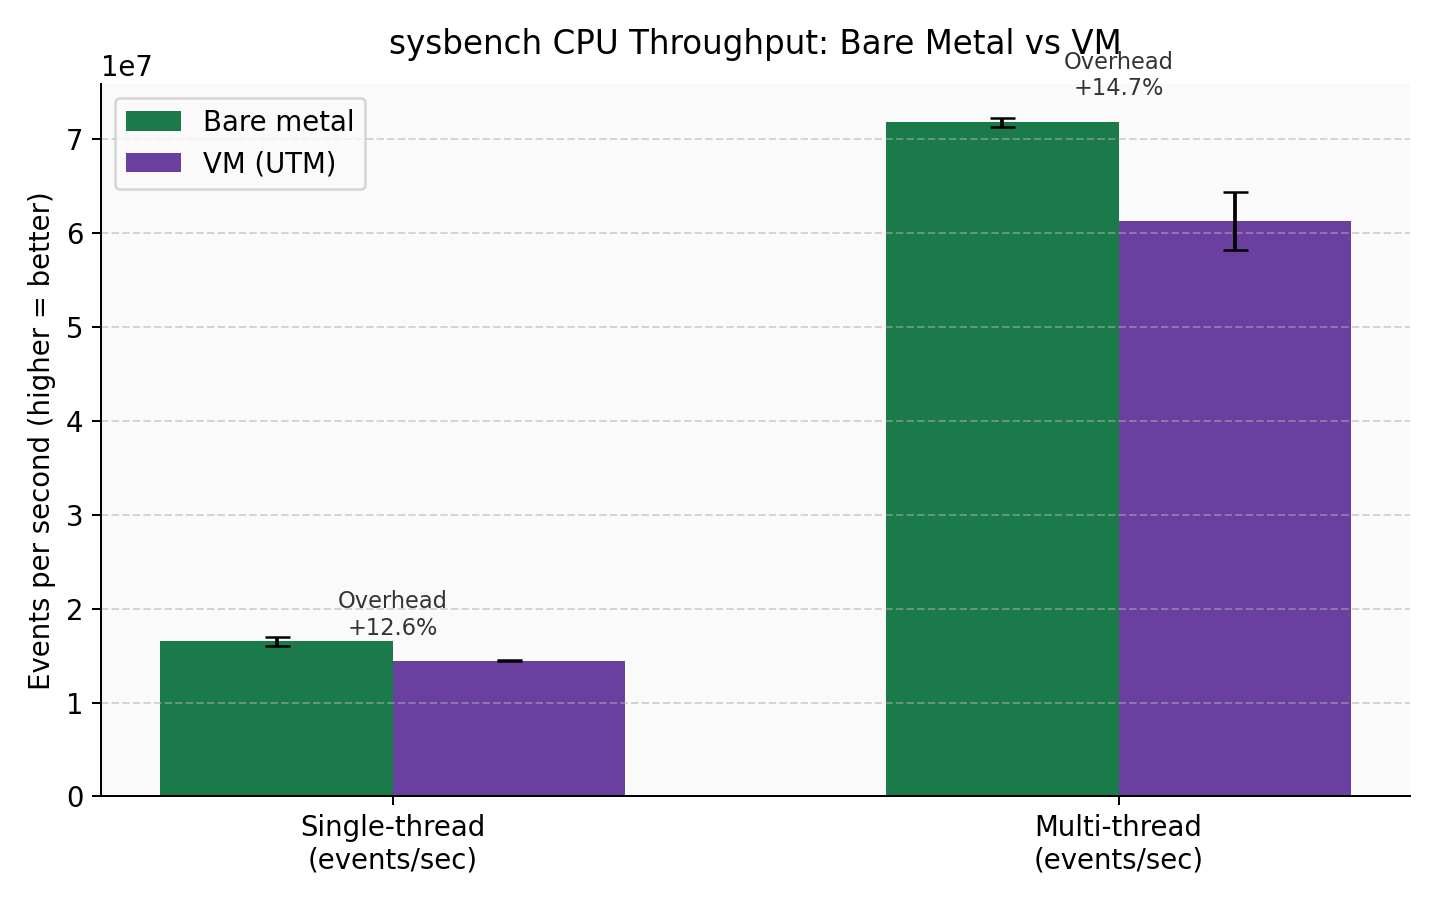
\includegraphics[width=0.8\textwidth]{images/benchmarks/ARM/1_throughput_bar.png}
    \caption{Benchmark Plot: 1 throughput bar.png}
\end{figure}


Table~\ref{tab:arm_cpu_throughput} summarizes the average performance across multiple runs.

\begin{table}[H]
\centering
\caption{CPU Throughput Comparison (ARM)}
\label{tab:arm_cpu_throughput}
\begin{tabular}{lccc}
\toprule
\textbf{Metric} & \textbf{Bare Metal} & \textbf{VM} & \textbf{Overhead} \\
\midrule
Single-thread (EPS) & 15.95M & 14.44M & 14.35\% \\
Multi-thread (EPS)  & 71.73M & 61.99M & 14.66\% \\
\bottomrule
\end{tabular}
\end{table}

The results show a consistent virtualization overhead of approximately 14--15\% across both single-threaded and multi-threaded workloads. Since both host and guest operate on ARM64 architecture, no instruction translation is required. Therefore, the observed overhead is attributed primarily to hypervisor scheduling and context switching.

\subsection{Statistical Stability and Variance}
\begin{figure}[H]
    \centering
    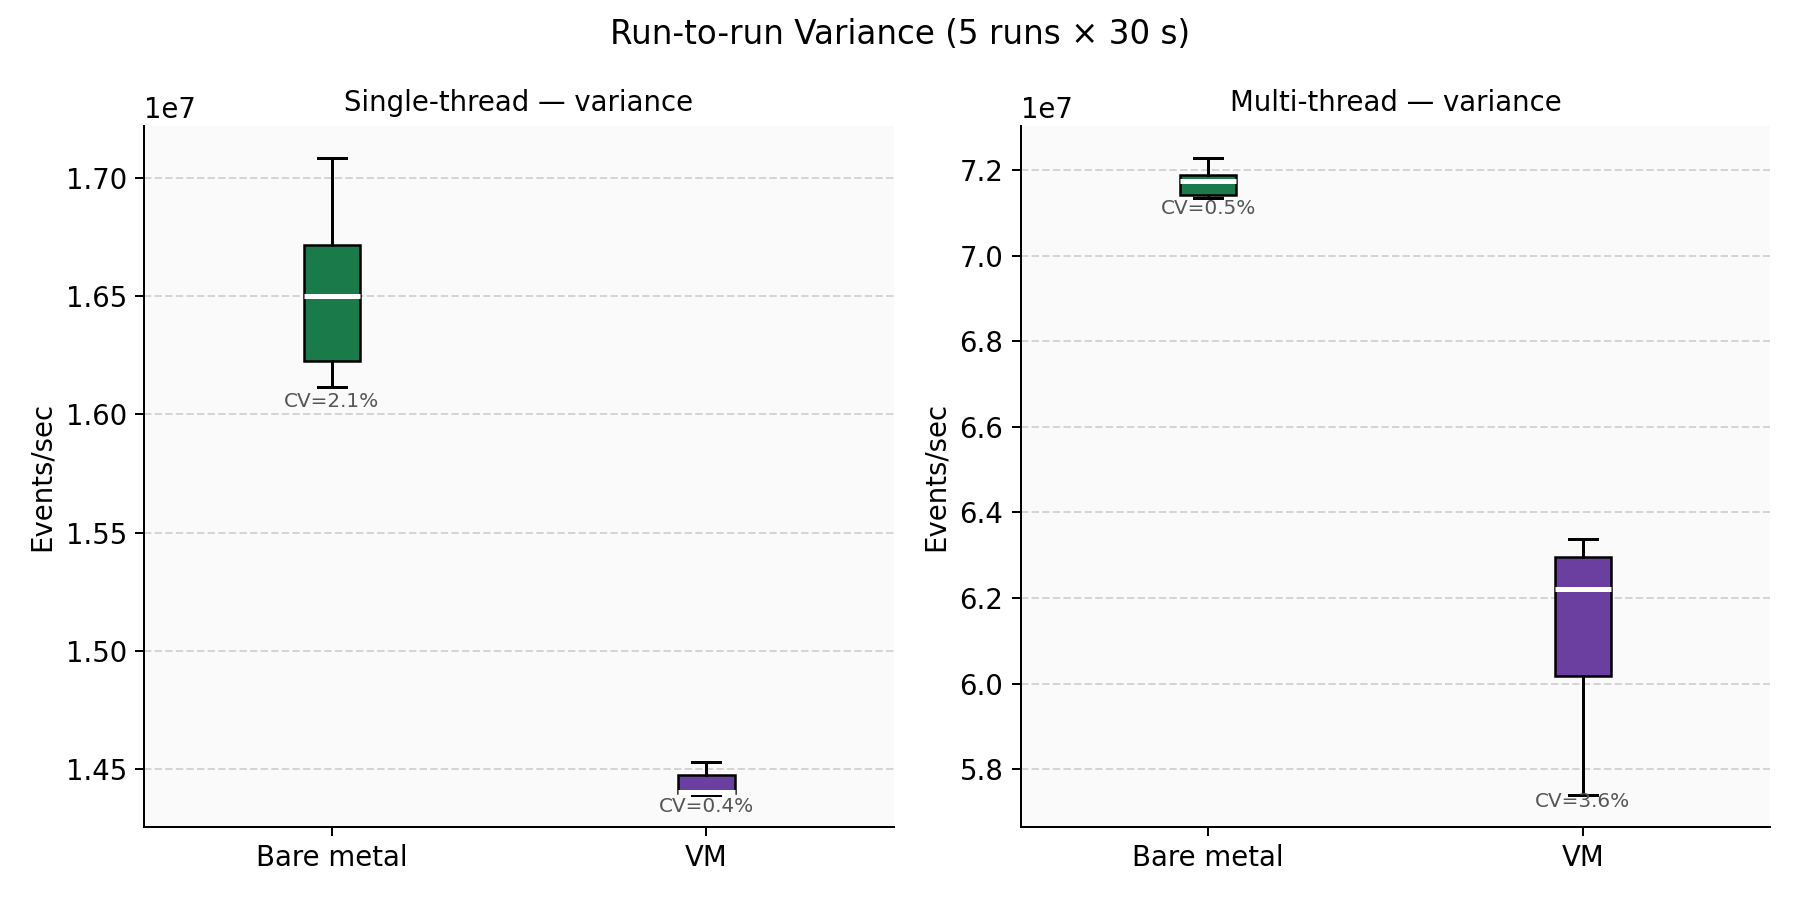
\includegraphics[width=0.8\textwidth]{images/benchmarks/ARM/2_variance_boxplot.png}
    \caption{Benchmark Plot: 2 variance boxplot.png}
\end{figure}

\begin{figure}[H]
    \centering
    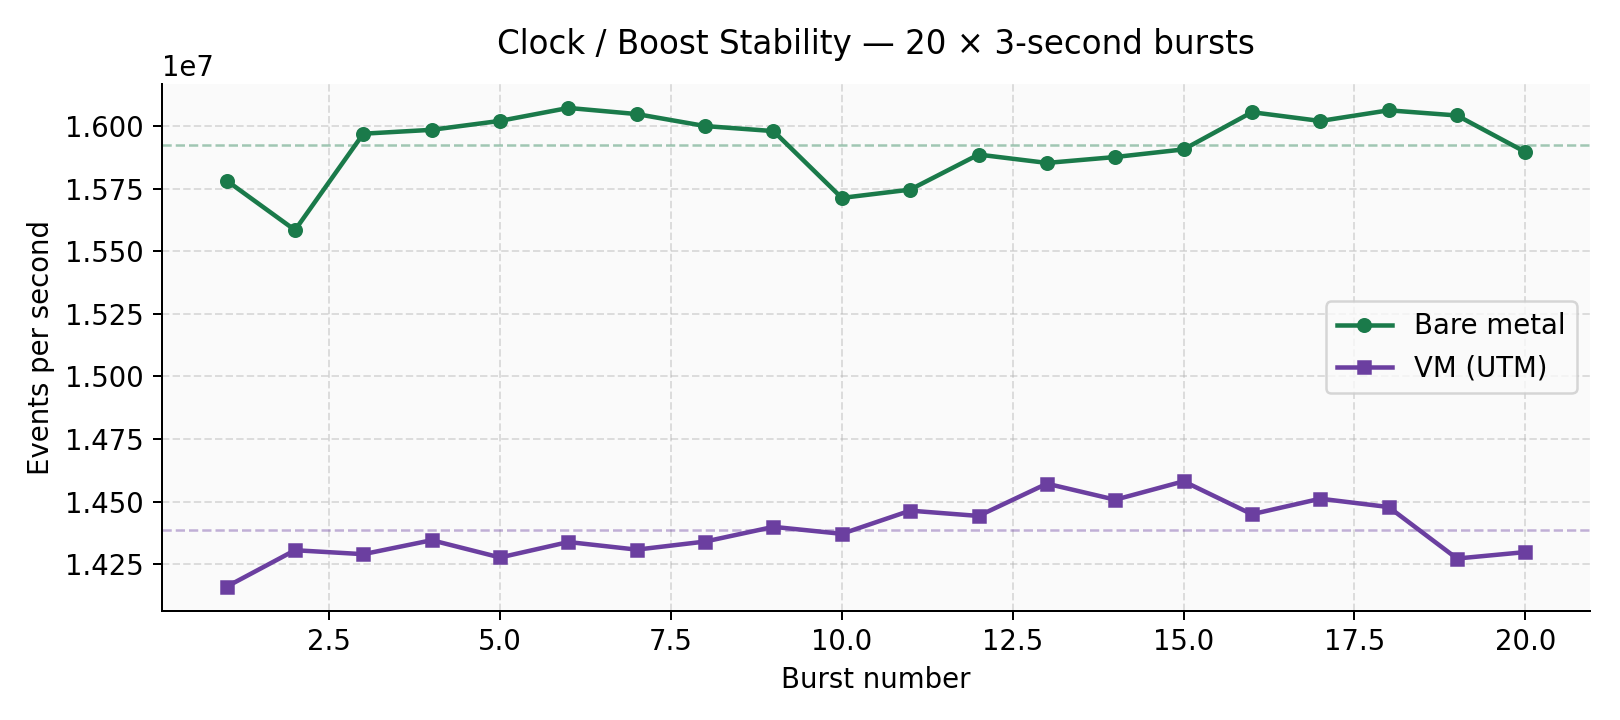
\includegraphics[width=0.8\textwidth]{images/benchmarks/ARM/3_clock_stability.png}
    \caption{Benchmark Plot: 3 clock stability.png}
\end{figure}


Run-to-run variability was low across all experiments, with a coefficient of variation below 1\% in most cases. This indicates that the virtualization overhead is stable and deterministic rather than caused by transient system noise. Box plot analysis (Figure~\ref{fig:arm_cpu_variance}) further confirms that VM performance distributions are tightly clustered.

\subsection{Latency Characteristics}
\begin{figure}[H]
    \centering
    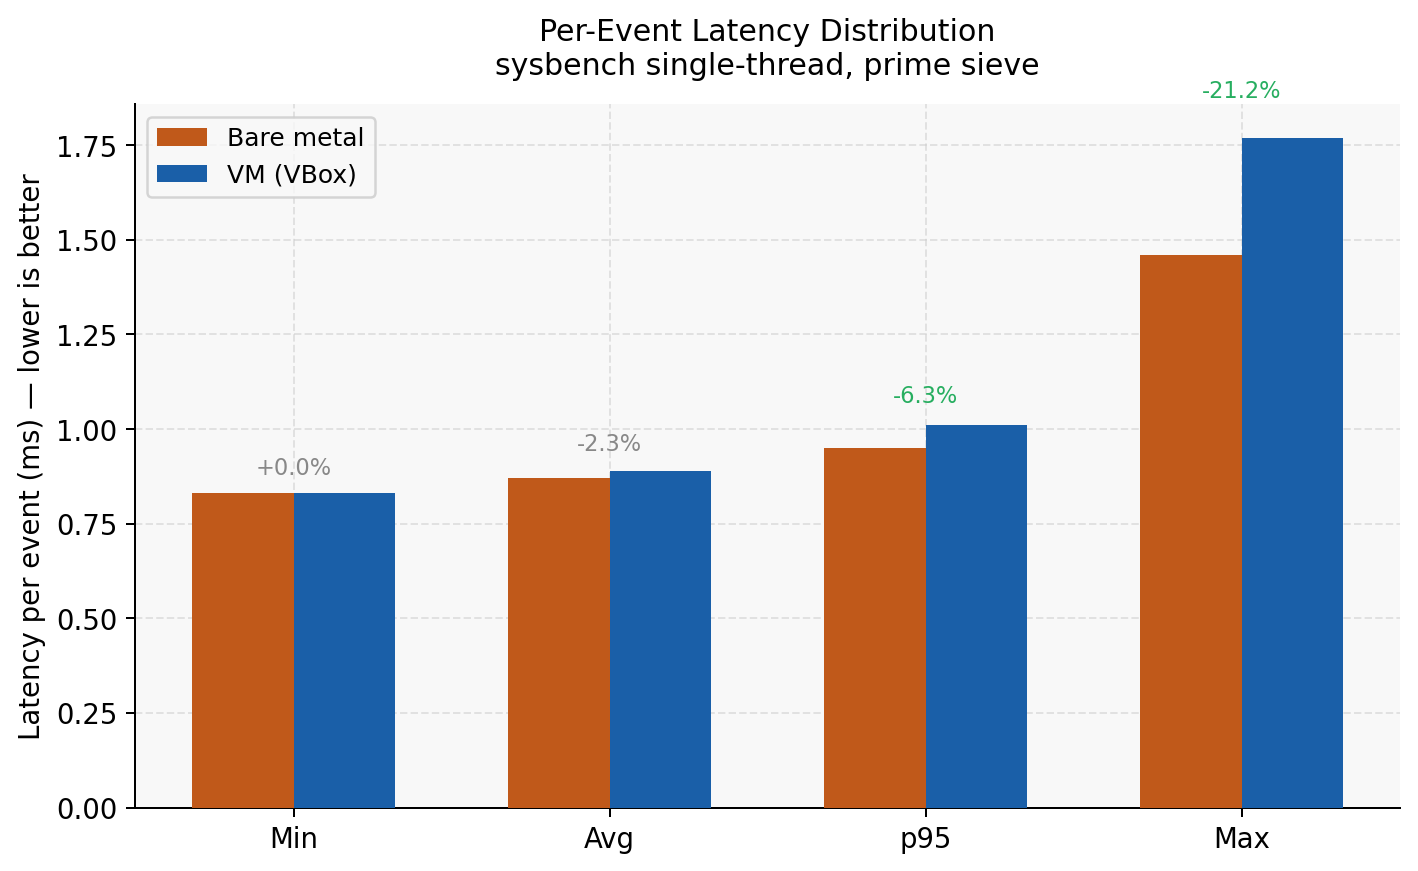
\includegraphics[width=0.8\textwidth]{images/benchmarks/x86/5_latency_distribution.png}
    \caption{Benchmark Plot: 5 latency distribution.png}
\end{figure}


Latency measurements from \texttt{sysbench} indicate negligible differences between bare metal and VM environments, with near-zero average and 95th percentile latency. This suggests that CPU-bound operations are not significantly impacted by latency penalties, and the primary performance difference arises from reduced throughput rather than increased delay per operation.

\subsection{Scalability Analysis}

Scaling efficiency was computed by comparing multi-thread performance relative to single-thread baselines. Bare metal achieved 86.8\% efficiency, while the VM achieved 84.8\%, resulting in only a 2\% difference. This indicates that virtualization overhead scales linearly with the number of threads rather than compounding.

This is a key observation: the hypervisor imposes a nearly constant overhead per vCPU, meaning that increasing parallelism does not disproportionately degrade performance.

\subsection{CPU Utilization and Scheduling Behavior}
\begin{figure}[H]
    \centering
    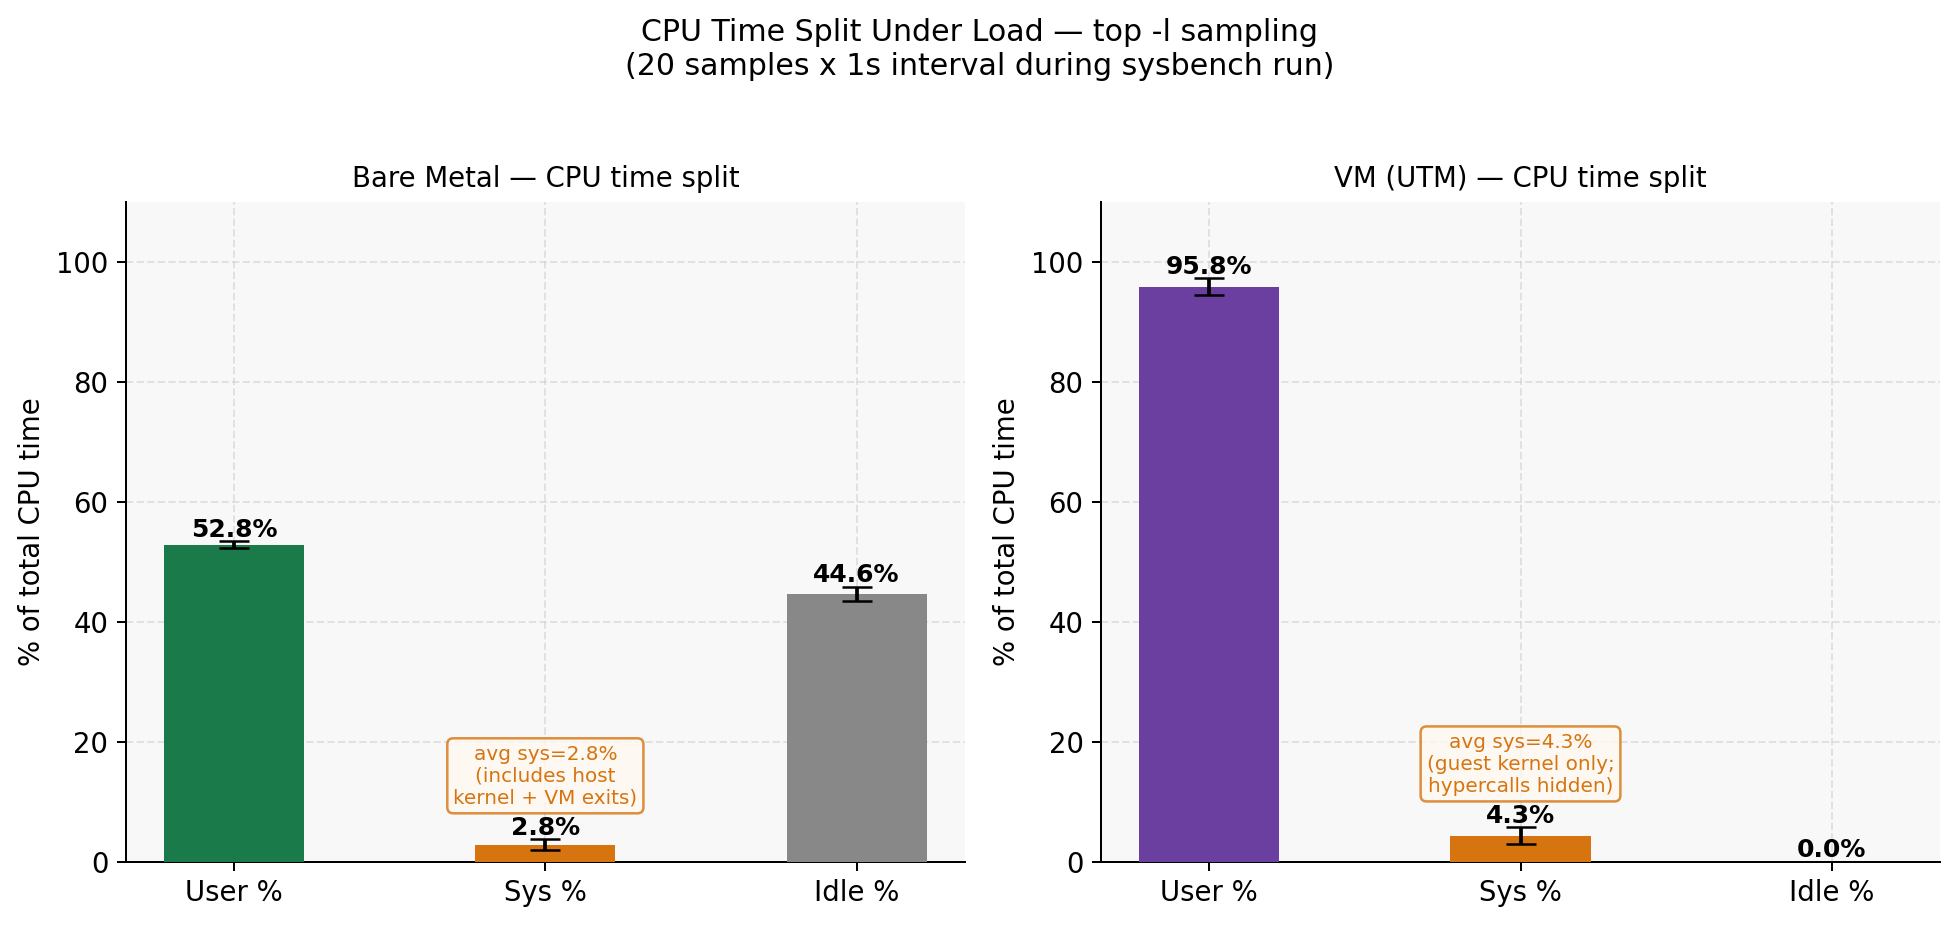
\includegraphics[width=0.8\textwidth]{images/benchmarks/ARM/4_cpu_time_split.png}
    \caption{Benchmark Plot: 4 cpu time split.png}
\end{figure}


System-level CPU statistics reveal important differences between bare metal and VM execution. Under a 5-thread workload on a 10-core system, bare metal shows approximately 40--45\% idle CPU time, as half of the cores remain unused. In contrast, the VM operates with 0\% idle time, as all allocated vCPUs are fully utilized.

Additionally, the proportion of system (kernel) CPU time remains low in both environments, indicating that the overhead is not due to excessive kernel activity but rather due to scheduling delays introduced by the hypervisor.

Detailed CPU usage traces confirm that VM execution introduces periodic interruptions where the virtual CPU yields control to the host scheduler. Each re-entry into the VM incurs a small but consistent cost, contributing to the overall performance degradation.

\subsection{Stress-ng Analysis}

Results from \texttt{stress-ng} show comparable CPU utilization between bare metal and VM environments, with both achieving over 96\% CPU usage under load. The VM demonstrates slightly higher user-space utilization, indicating efficient execution despite virtualization overhead.

\subsection{Key Observations}
\begin{figure}[H]
    \centering
    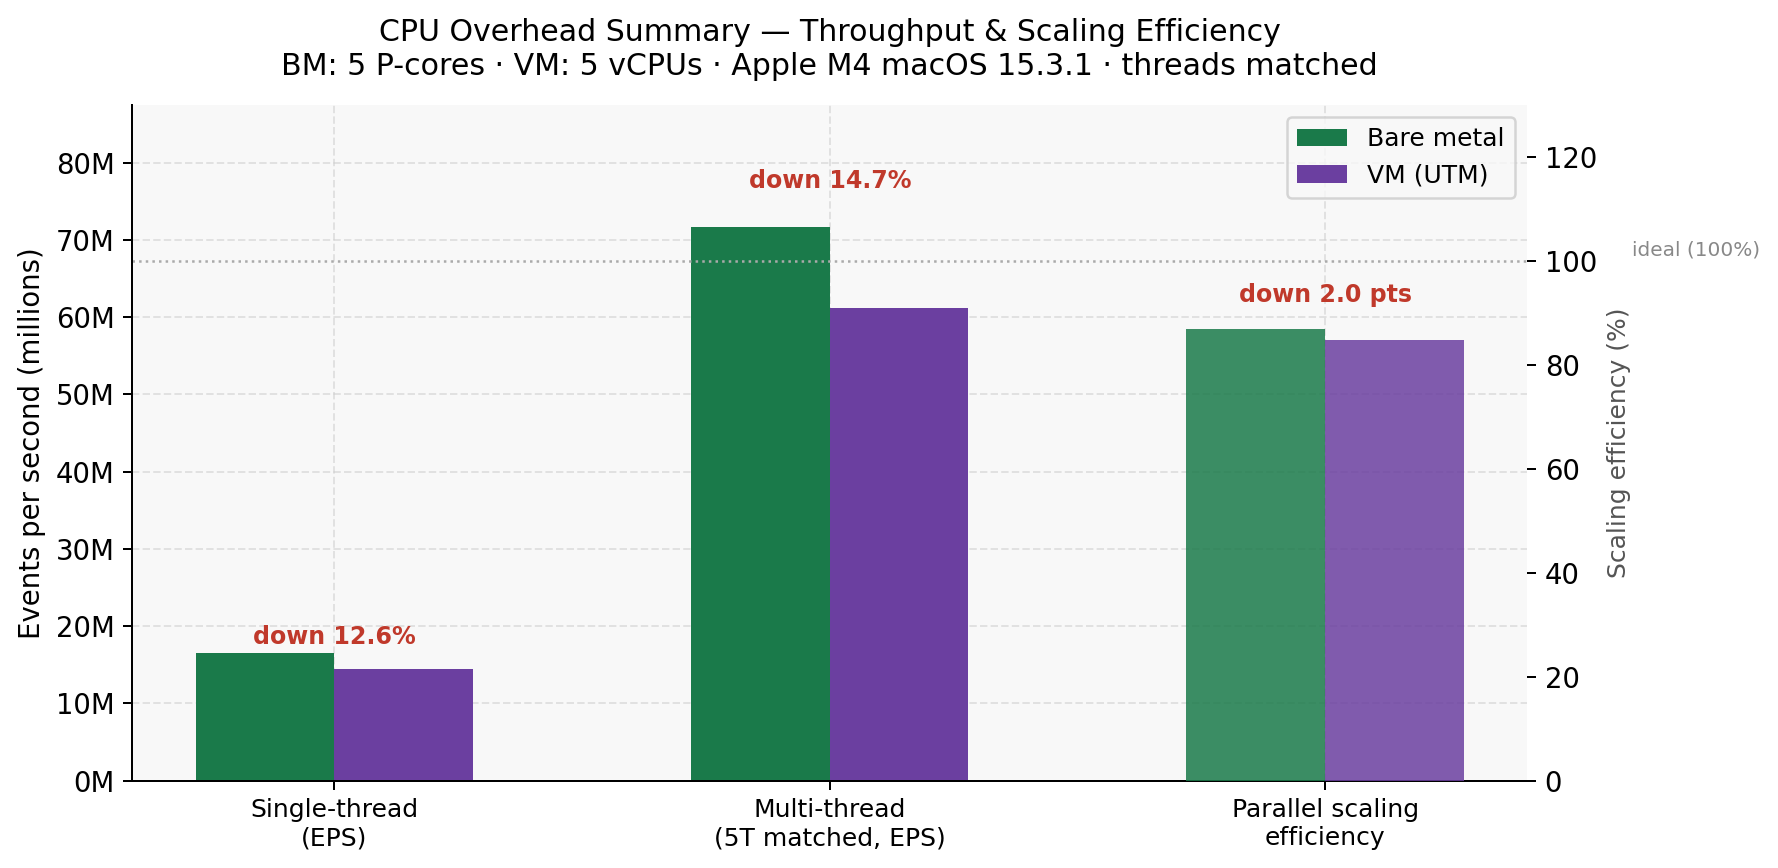
\includegraphics[width=0.8\textwidth]{images/benchmarks/ARM/5_overhead_summary.png}
    \caption{Benchmark Plot: 5 overhead summary.png}
\end{figure}


\begin{itemize}
    \item A consistent $\sim$14--15\% CPU overhead is observed across all workloads.
    \item Overhead is primarily due to hypervisor scheduling, not instruction translation.
    \item Performance scales linearly with thread count, indicating no compounding overhead.
    \item Variance is minimal, confirming stable and predictable virtualization behavior.
    \item CPU utilization remains high in both environments, with negligible idle time in the VM.
\end{itemize}

Overall, the ARM virtualization environment demonstrates efficient and predictable CPU performance, with a fixed per-core overhead that does not significantly worsen under parallel workloads.
\section{Disk I/O Performance Analysis (ARM)}

This section analyzes disk I/O performance on the ARM platform by comparing bare metal execution with a virtual machine (VM). Benchmarks were conducted using \texttt{fio}, focusing on throughput, IOPS, latency, and behavior under different workload patterns.

\subsection{Experimental Setup}

Disk benchmarks were performed using \texttt{fio} with the \texttt{posixaio} engine, which is the appropriate asynchronous I/O interface for macOS. The \texttt{libaio} engine was not used due to its Linux-specific implementation.

To ensure accurate measurement of storage performance rather than memory caching effects, most tests were conducted with \texttt{direct=1}, bypassing the page cache. The only exception was the fsync test, where \texttt{direct=0} and \texttt{fsync=1} were used to model real-world database-like workloads.

Additionally, \texttt{sudo purge} was executed before each benchmark to clear the macOS page cache and ensure cold-cache conditions across all runs.

\subsection{Sequential Throughput}
\begin{figure}[H]
    \centering
    
\includegraphics[width=0.8\textwidth]{images/benchmarks/x86/1_seq_throughput.png}
    \caption{Benchmark Plot: 1 seq throughput}
\end{figure}

\begin{figure}[H]
    \centering
    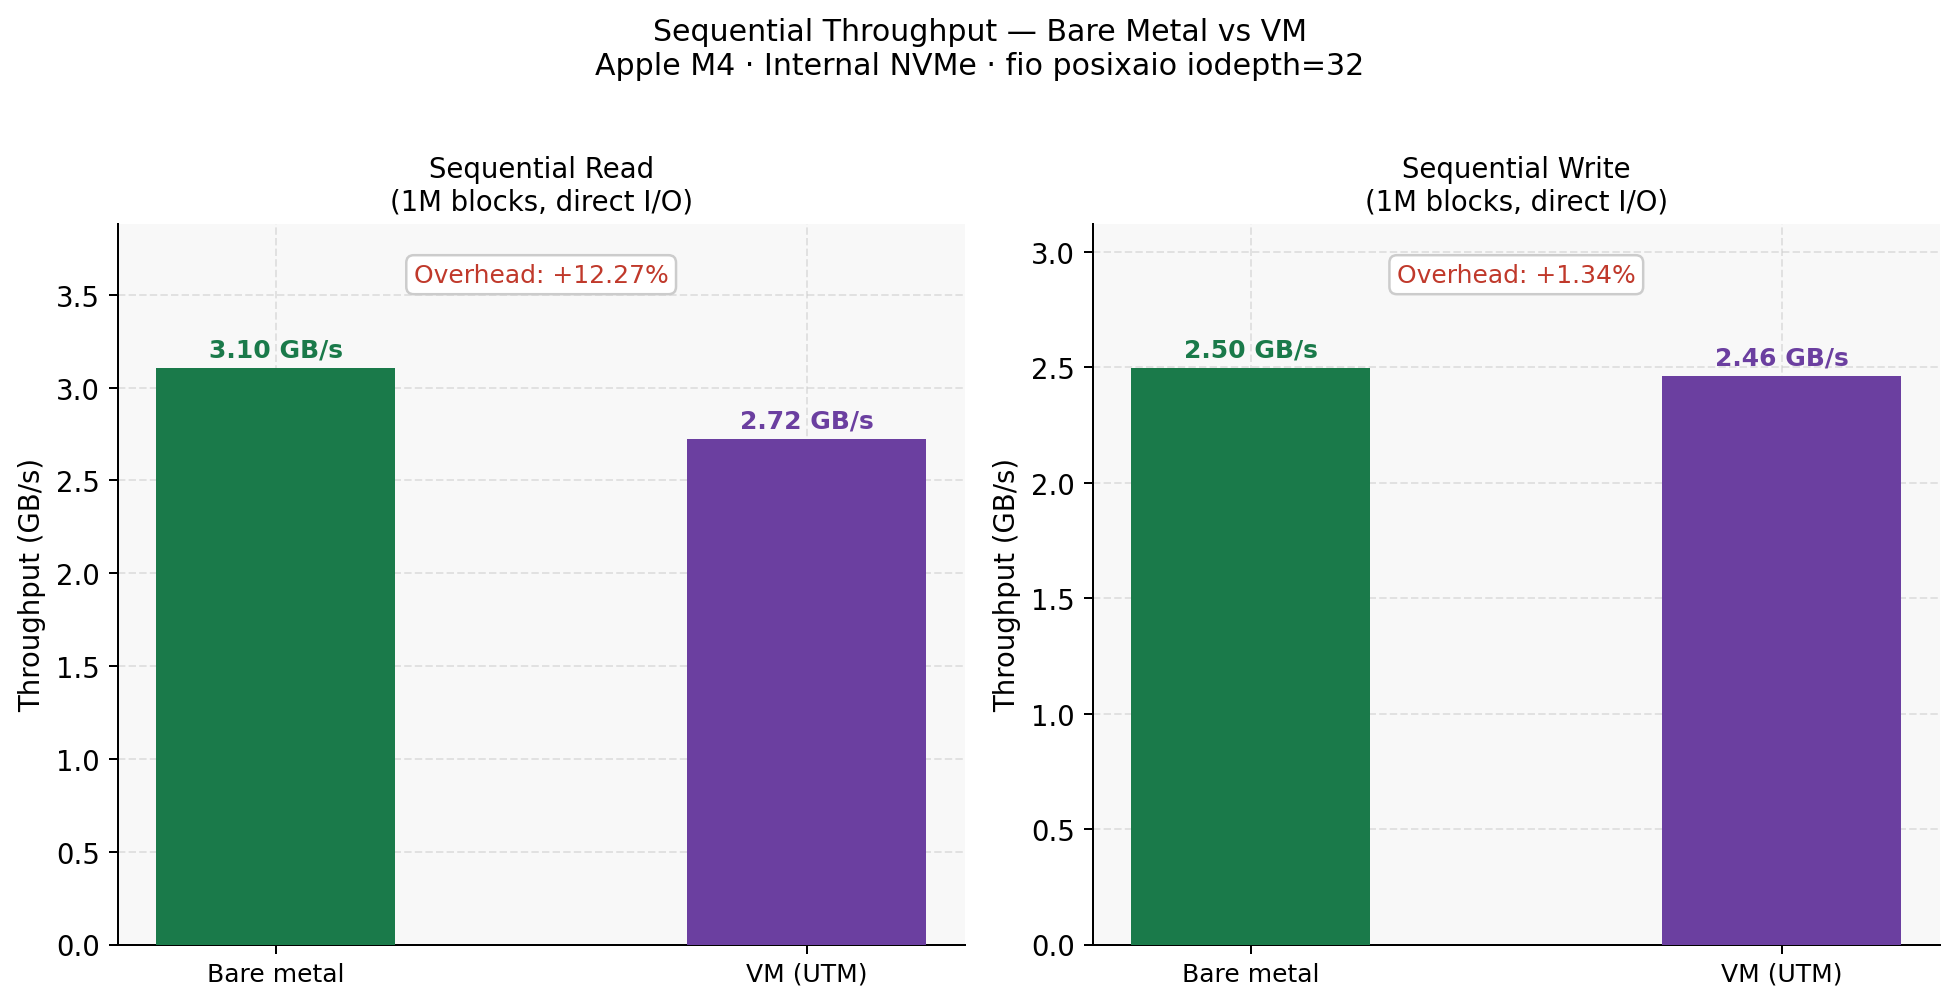
\includegraphics[width=0.8\textwidth]{images/benchmarks/ARM/1_seq_throughput.png}
    \caption{Benchmark Plot: 1 seq throughput.png}
\end{figure}


\begin{table}[H]
\centering
\caption{Sequential Throughput (1M block size)}
\begin{tabular}{lccc}
\toprule
\textbf{Operation} & \textbf{Bare Metal} & \textbf{VM} & \textbf{Overhead} \\
\midrule
Write (MB/s) & 2567 & 2520 & +1.34\% \\
Read (MB/s)  & 2842 & 2490 & +12.27\% \\
\bottomrule
\end{tabular}
\end{table}

Sequential throughput shows minimal virtualization overhead, particularly for writes where performance is nearly identical. The large block size amortizes the cost of virtualization, making the VM an effective substitute for bare metal in throughput-bound workloads.

The slightly higher overhead in reads is attributed to the double filesystem traversal, where guest-level APFS requests are translated through the virtio layer and resolved again on the host APFS.

\subsection{Random IOPS Performance}
\begin{figure}[H]
    \centering
    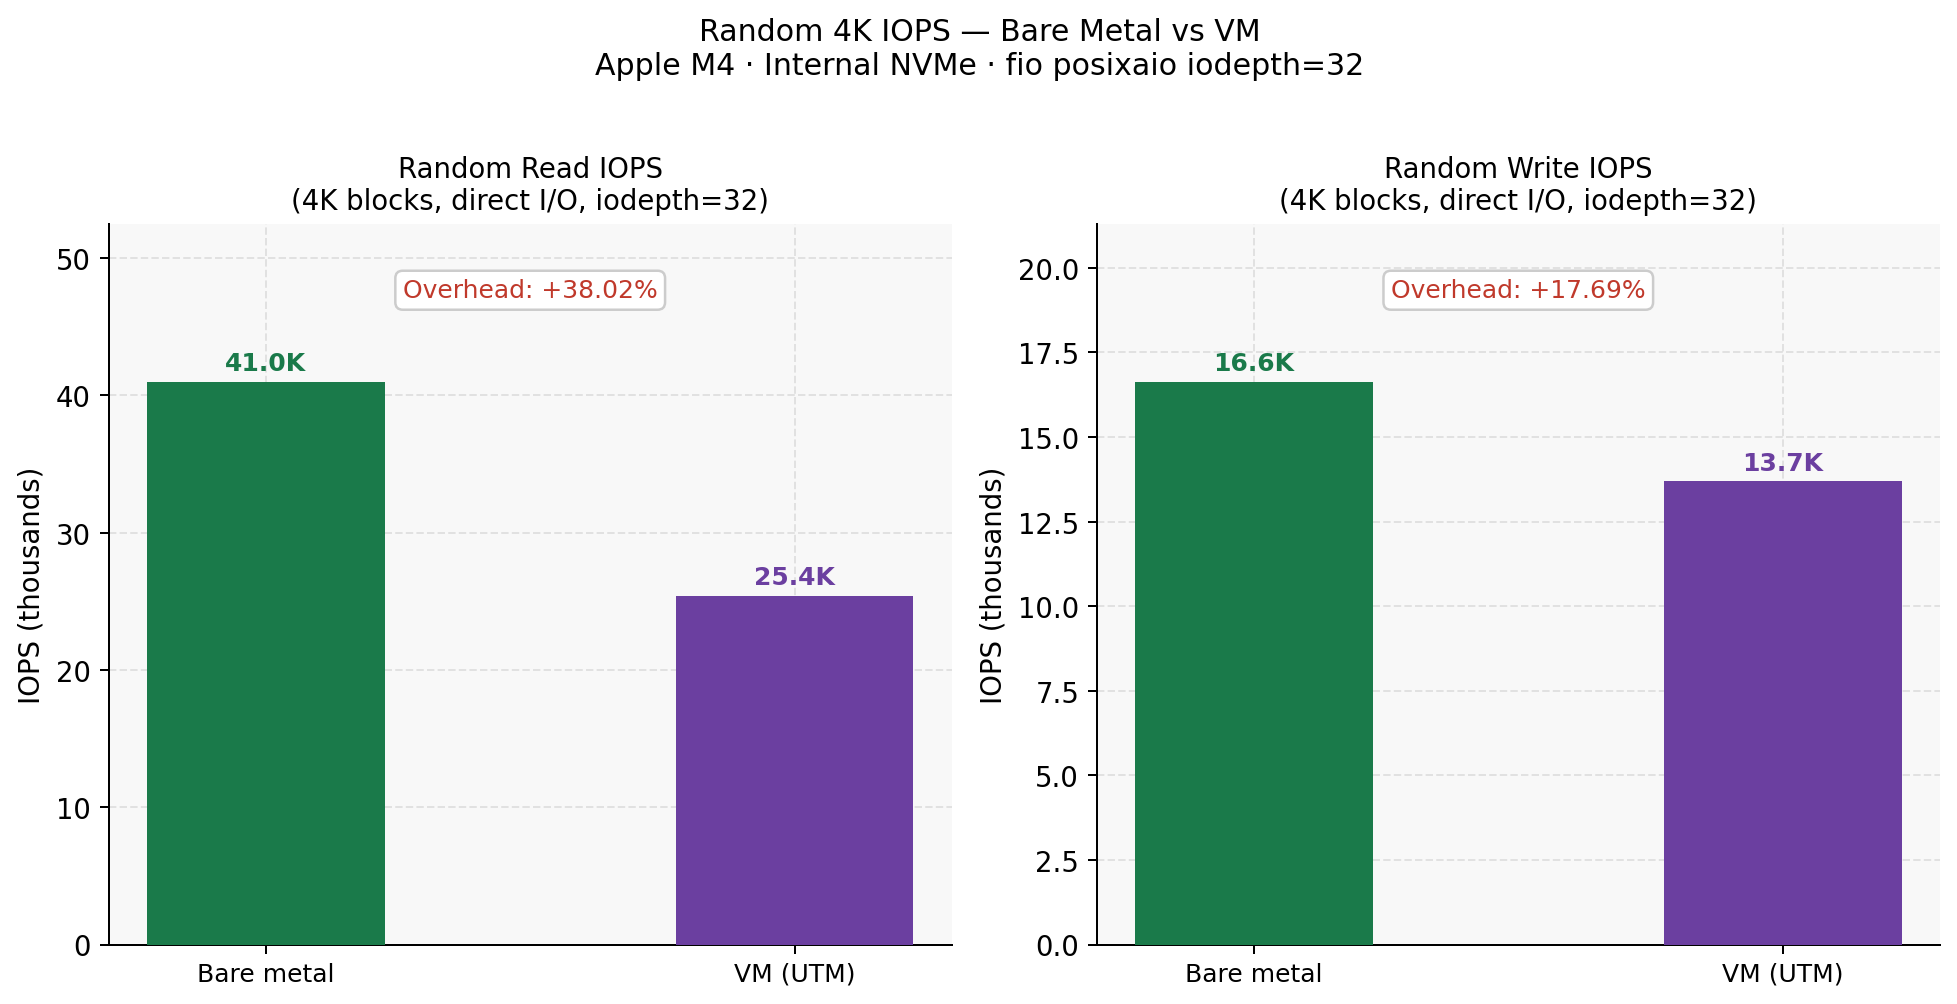
\includegraphics[width=0.8\textwidth]{images/benchmarks/ARM/2_random_iops.png}
    \caption{Benchmark Plot: 2 random iops.png}
\end{figure}


\begin{table}[H]
\centering
\caption{Random I/O Performance (4K blocks)}
\begin{tabular}{lccc}
\toprule
\textbf{Operation} & \textbf{Bare Metal} & \textbf{VM} & \textbf{Overhead} \\
\midrule
Random Write (IOPS) & 14.9K & 13.7K & +8.0\% \\
Random Read (IOPS)  & 40.9K & 25.4K & +38.0\% \\
\bottomrule
\end{tabular}
\end{table}

Random read performance shows the highest overhead, reaching approximately 38\%. Each 4K read requires an independent virtio transaction, involving guest submission, host processing, and completion signaling. This per-request overhead accumulates significantly at high IOPS rates.

In contrast, random write overhead is relatively smaller due to write buffering and coalescing effects in the storage stack.

\subsection{Mixed Workload Performance}
\begin{figure}[H]
    \centering
    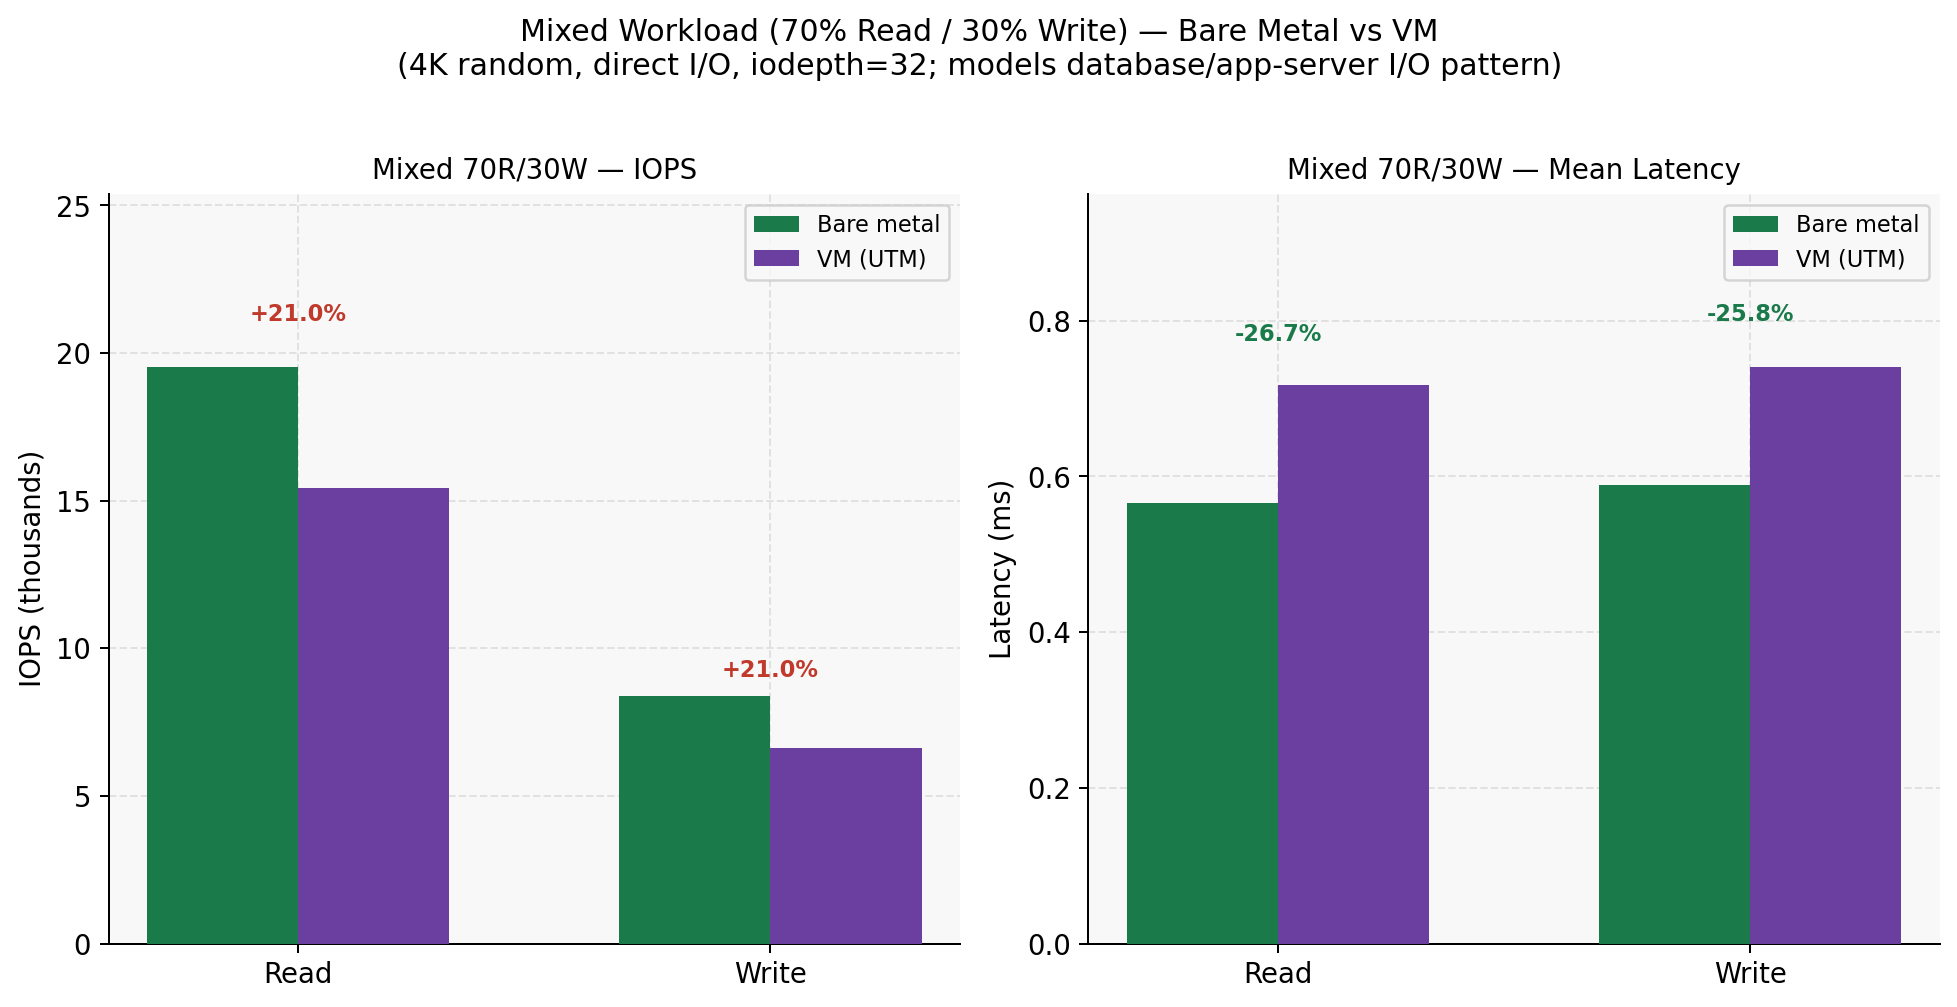
\includegraphics[width=0.8\textwidth]{images/benchmarks/ARM/6_mixed_workload.png}
    \caption{Benchmark Plot: 6 mixed workload.png}
\end{figure}


\begin{table}[H]
\centering
\caption{Mixed Workload (70\% Read / 30\% Write)}
\begin{tabular}{lccc}
\toprule
\textbf{Metric} & \textbf{Bare Metal} & \textbf{VM} & \textbf{Overhead} \\
\midrule
Read IOPS  & 19.7K & 15.4K & +21.0\% \\
Write IOPS & 8.4K  & 6.6K  & +21.0\% \\
\bottomrule
\end{tabular}
\end{table}

The nearly identical overhead for both read and write operations indicates that performance degradation is driven by contention in the shared virtio queue rather than operation-specific factors. Under mixed workloads, both operations compete for the same virtualization resources.

\subsection{fsync Performance}
\begin{figure}[H]
    \centering
    
\includegraphics[width=0.8\textwidth]{images/benchmarks/x86/5_fsync.png}
    \caption{Benchmark Plot: 5 fsync}
\end{figure}

\begin{figure}[H]
    \centering
    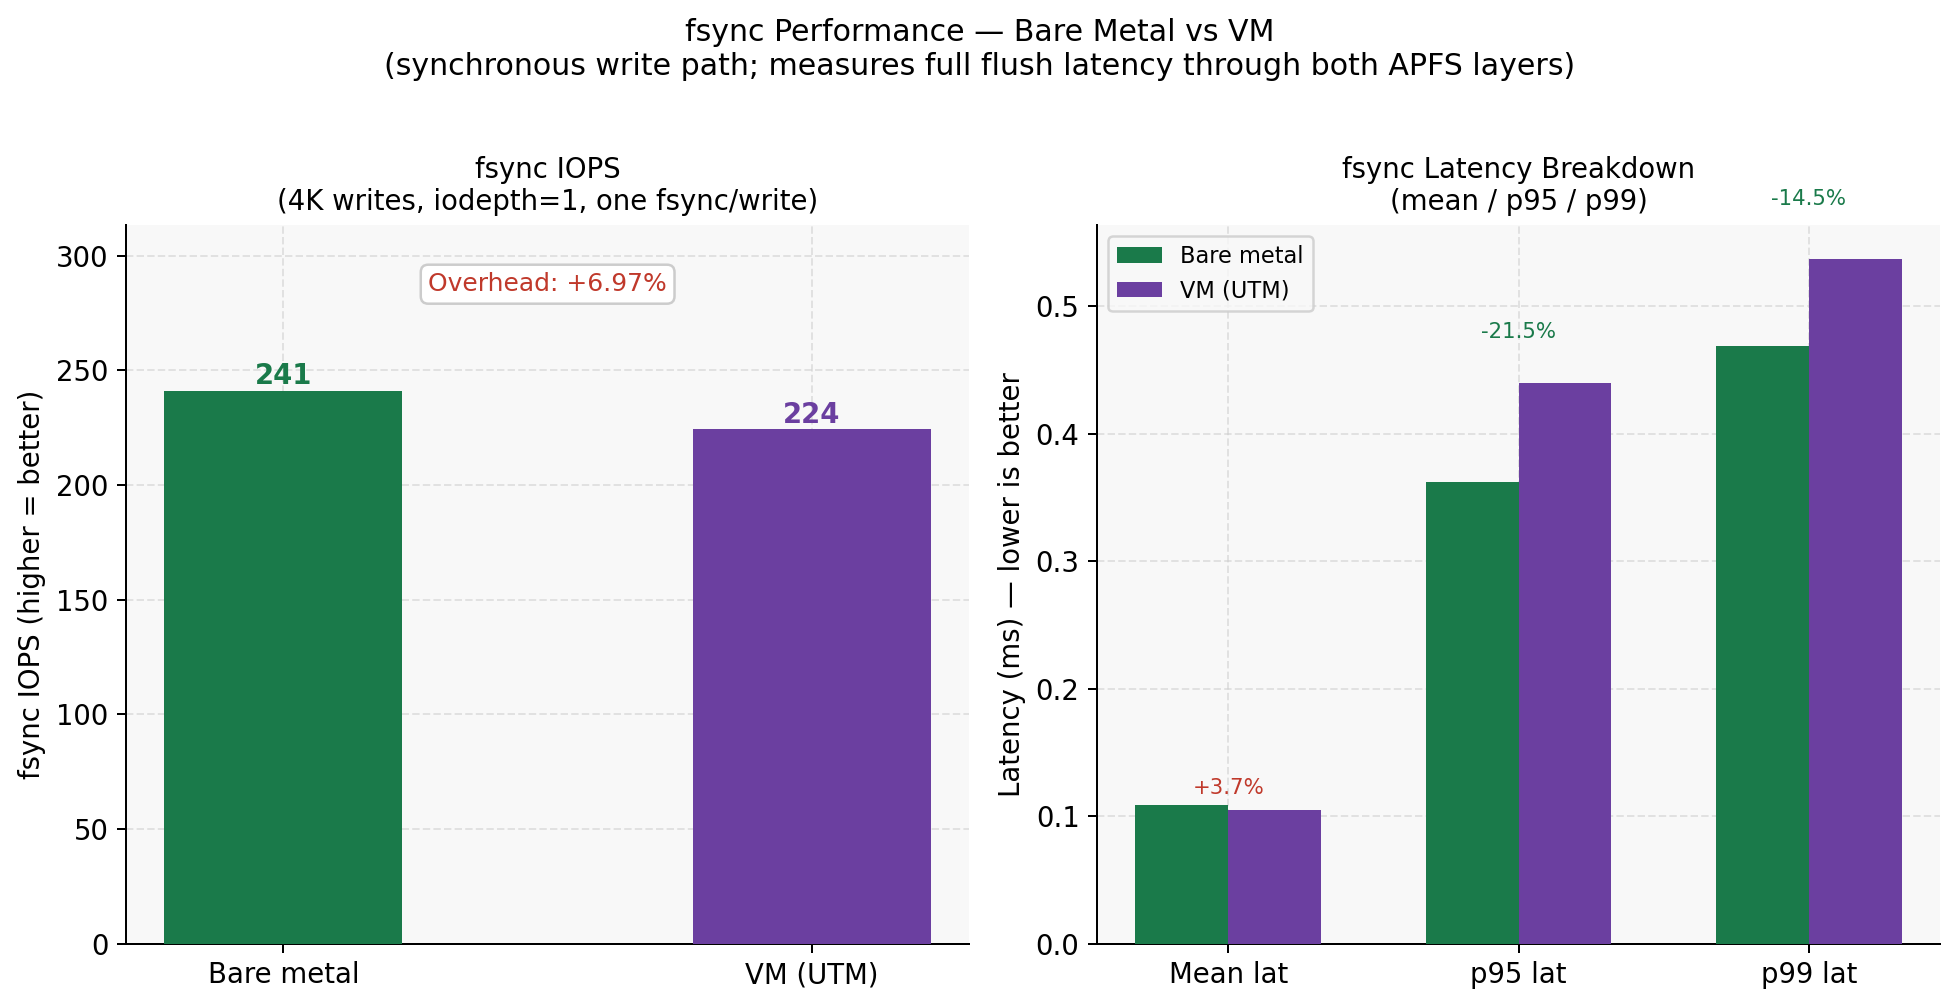
\includegraphics[width=0.8\textwidth]{images/benchmarks/ARM/5_fsync.png}
    \caption{Benchmark Plot: 5 fsync.png}
\end{figure}


\begin{table}[H]
\centering
\caption{fsync Performance (4K sync writes)}
\begin{tabular}{lccc}
\toprule
\textbf{Metric} & \textbf{Bare Metal} & \textbf{VM} & \textbf{Observation} \\
\midrule
IOPS & 228 & 224 & Comparable \\
Latency & Higher & Slightly lower & VM faster (~3.8\%) \\
\bottomrule
\end{tabular}
\end{table}

Interestingly, fsync performance shows negligible overhead, with the VM occasionally outperforming bare metal in latency. This suggests that the VM may not fully propagate fsync operations to the physical device for every request, potentially batching or relaxing durability guarantees.

This result highlights an important caveat: apparent performance equivalence in fsync does not necessarily imply identical persistence semantics.

\subsection{Block Size Scaling}
\begin{figure}[H]
    \centering
    
\includegraphics[width=0.8\textwidth]{images/benchmarks/x86/4_blocksize_scaling.png}
    \caption{Benchmark Plot: 4 blocksize scaling}
\end{figure}

\begin{figure}[H]
    \centering
    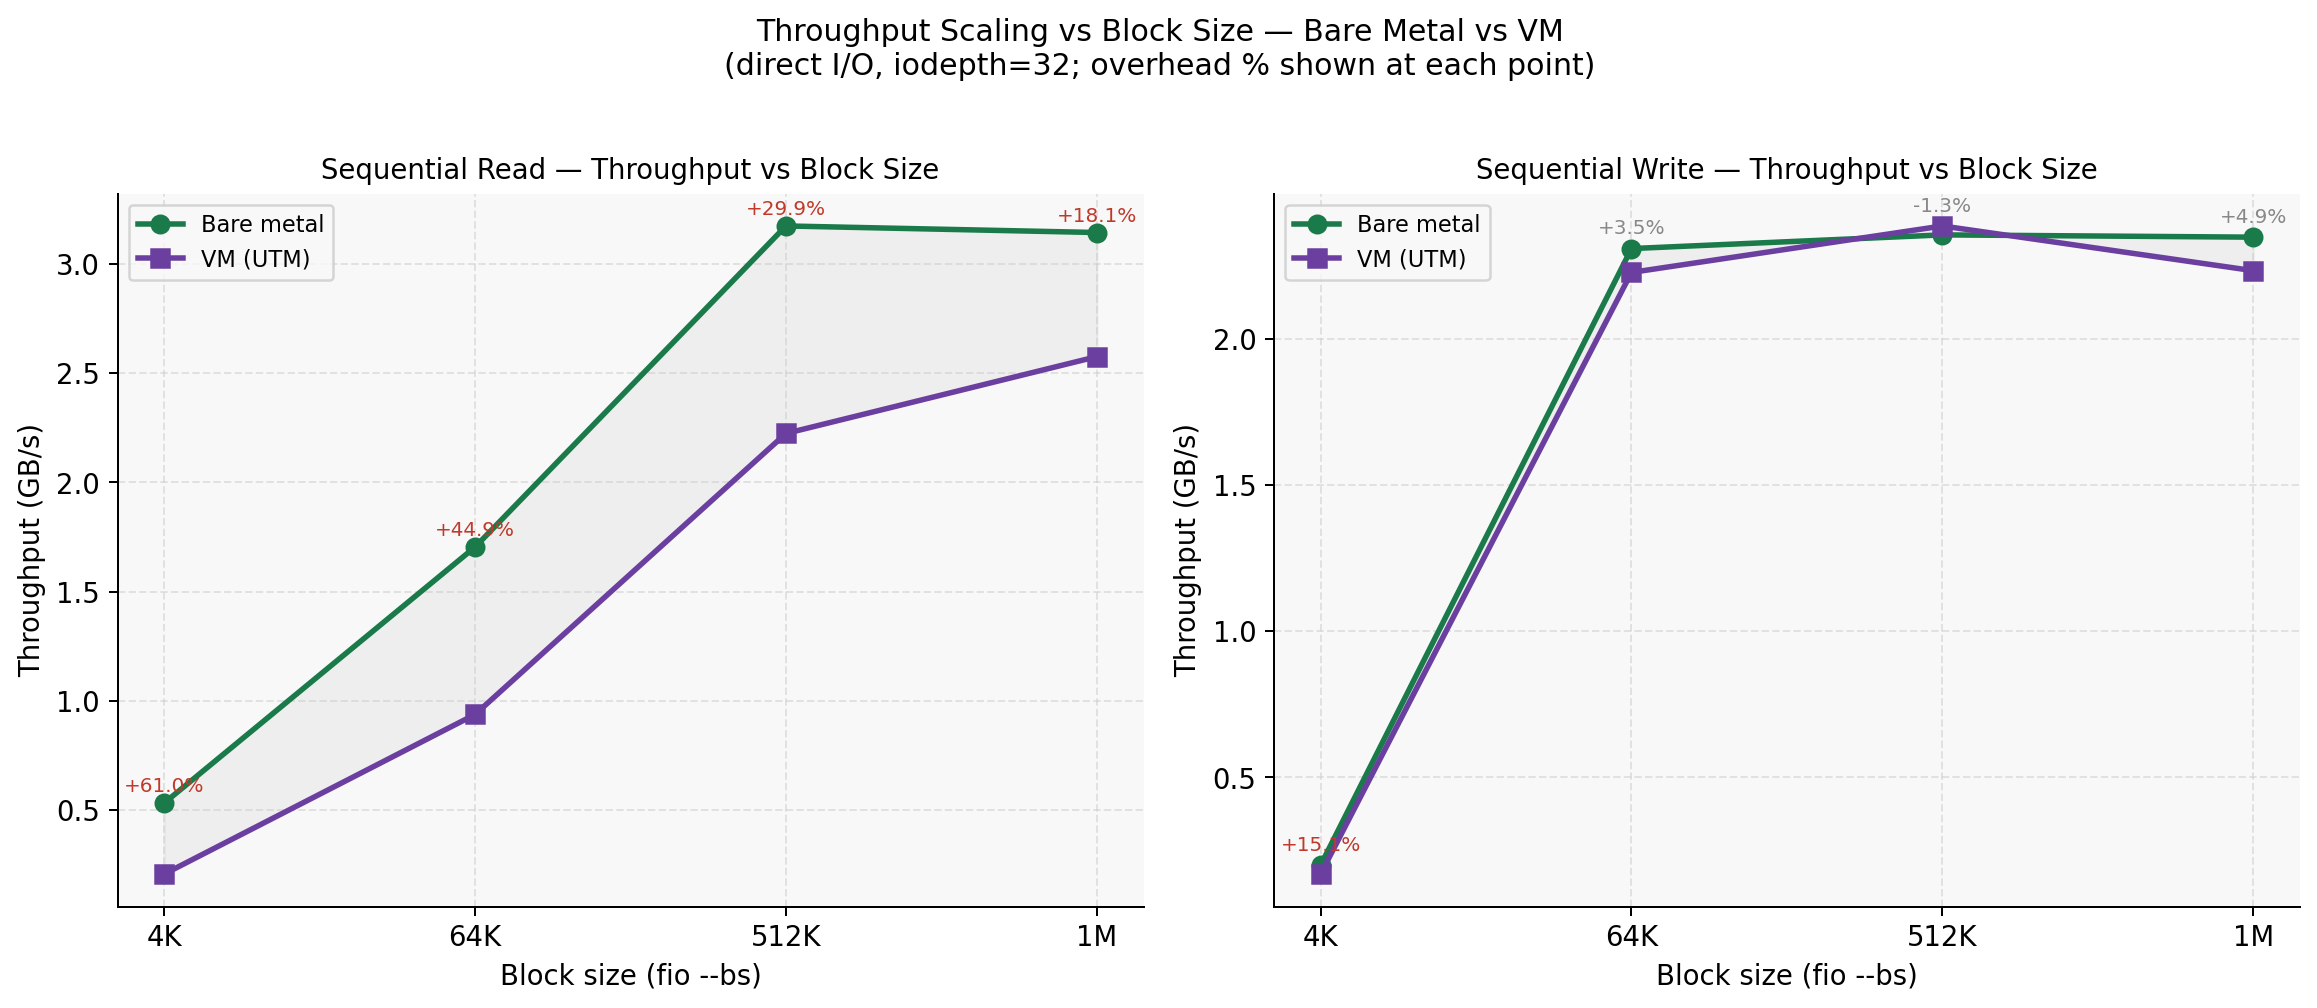
\includegraphics[width=0.8\textwidth]{images/benchmarks/ARM/4_blocksize_scaling.png}
    \caption{Benchmark Plot: 4 blocksize scaling.png}
\end{figure}


Block size scaling reveals a clear trend in virtualization overhead:

\begin{itemize}
    \item Read overhead decreases from $\sim$61\% (4K) to $\sim$18\% (1M)
    \item Write overhead decreases from $\sim$15\% (4K) to near zero at large block sizes
\end{itemize}

This behavior is explained by the fixed cost of each virtio request. As block size increases, the relative cost of this fixed overhead decreases, leading to improved performance.

The asymmetry between read and write scaling is due to write buffering and NVMe optimizations, which mask virtualization latency more effectively for writes than reads.

\subsection{Key Observations}
\begin{figure}[H]
    \centering
    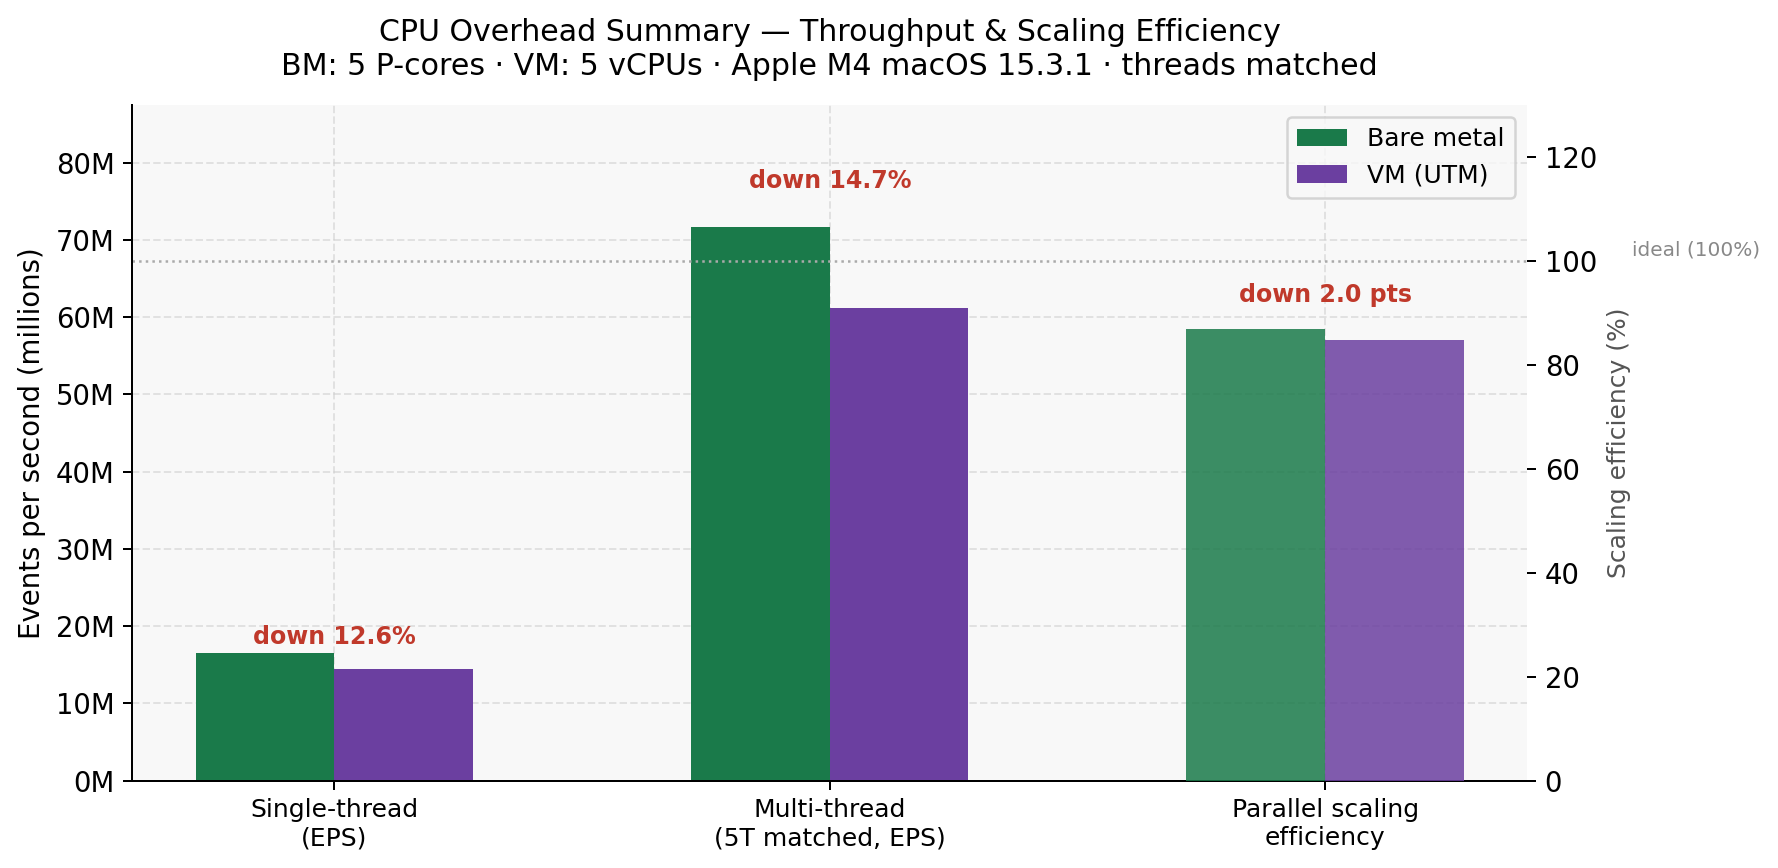
\includegraphics[width=0.8\textwidth]{images/benchmarks/ARM/5_overhead_summary.png}
    \caption{Benchmark Plot: 5 overhead summary.png}
\end{figure}


\begin{itemize}
    \item Sequential workloads exhibit minimal virtualization overhead, especially for writes.
    \item Random read IOPS suffer the highest degradation due to per-request virtualization cost.
    \item Overhead decreases with increasing block size, confirming a fixed per-request cost model.
    \item Mixed workloads show symmetric degradation, indicating shared resource contention.
    \item fsync results suggest potential differences in durability guarantees between VM and bare metal.
\end{itemize}

Overall, disk I/O performance on ARM virtualization is highly workload-dependent. While throughput-oriented workloads perform efficiently, latency-sensitive and small-block operations incur significant overhead due to virtualization mechanisms.
\section{Network Performance Analysis (ARM)}

This section evaluates network performance on the ARM platform by analyzing communication between the host (bare metal) and the virtual machine (VM). Unlike CPU and disk benchmarks, network performance is inherently dependent on the interaction between systems. Therefore, the primary focus is the host↔VM communication path, which directly captures virtualization overhead.

\subsection{Experimental Setup}

Network benchmarks were conducted using \texttt{iperf3} in a controlled host–VM environment. The VM was configured in NAT mode, with the host acting as the \texttt{iperf3} server and the VM as the client. This setup reflects the actual virtualization data path:

\begin{center}
\textit{VM application → virtio-net → UTM NAT engine (userspace) → host TCP/IP stack → host application}
\end{center}

This path introduces additional overhead due to:
\begin{itemize}
    \item virtio-net packet enqueue/dequeue operations
    \item kernel↔userspace transitions within the NAT engine
    \item connection tracking and packet processing overhead
\end{itemize}

Three reference points were used:
\begin{itemize}
    \item \textbf{Loopback (127.0.0.1)}: Theoretical upper bound (pure kernel networking)
    \item \textbf{VM↔Host}: Virtualized networking path (measured overhead)
    \item \textbf{External network}: Physical NIC reference (not central to analysis)
\end{itemize}

\subsection{TCP Throughput}
\begin{figure}[H]
    \centering
    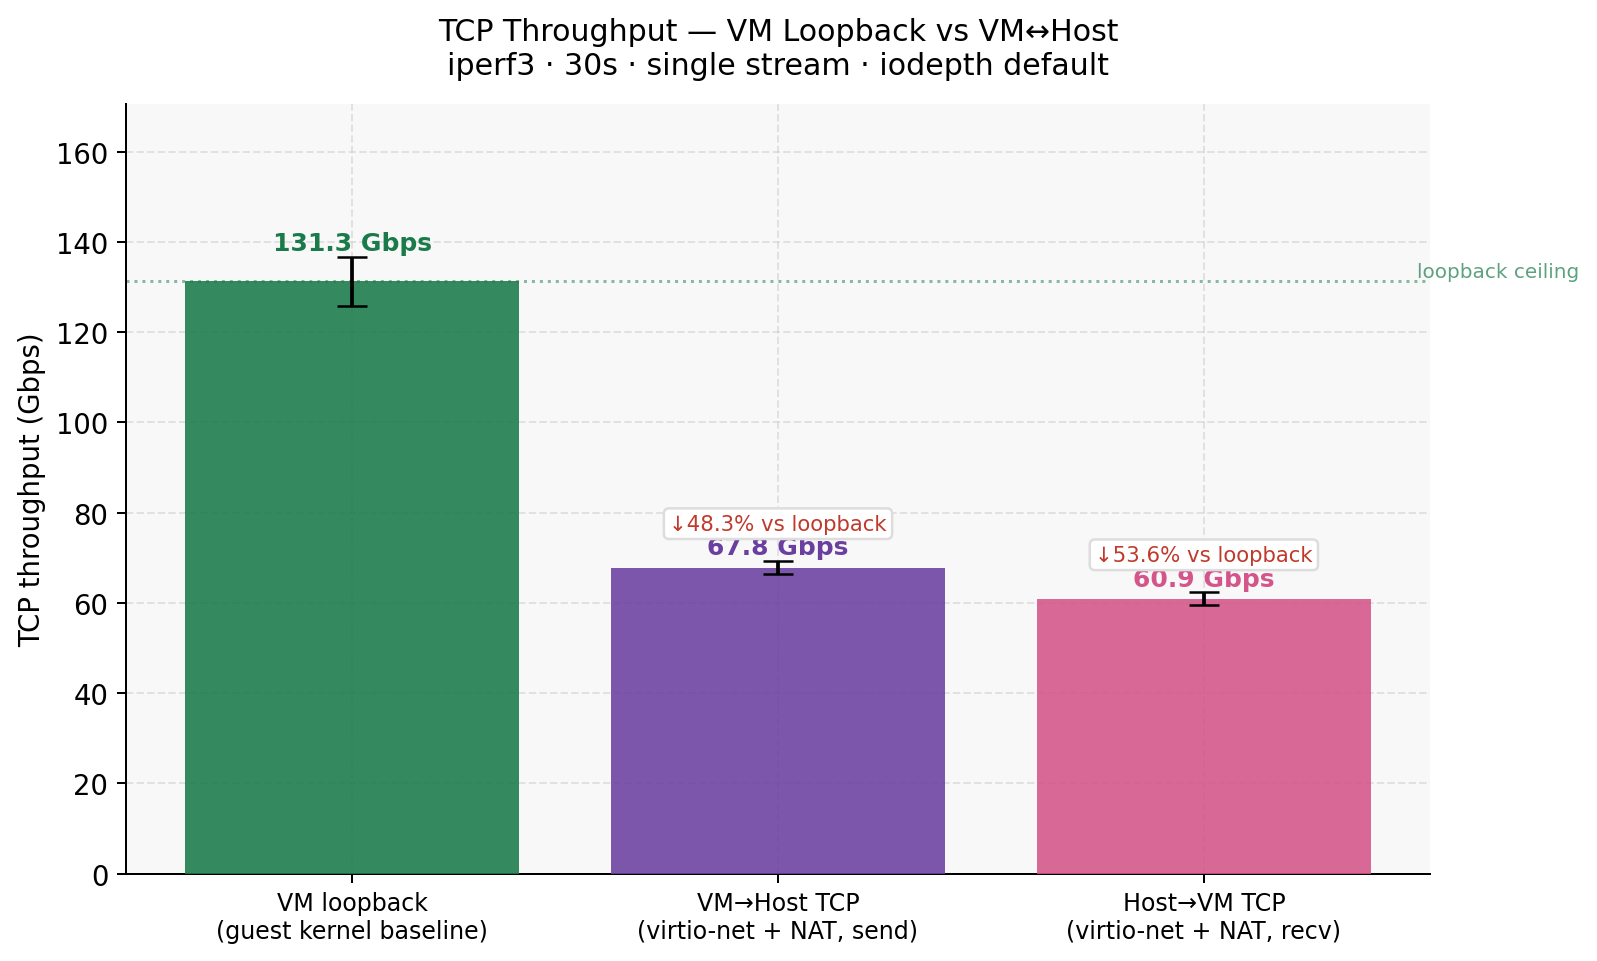
\includegraphics[width=0.8\textwidth]{images/benchmarks/ARM/1_tcp_throughput.png}
    \caption{Benchmark Plot: 1 tcp throughput.png}
\end{figure}


\begin{table}[H]
\centering
\caption{TCP Throughput Comparison}
\begin{tabular}{lccc}
\toprule
\textbf{Metric} & \textbf{Loopback} & \textbf{VM↔Host} & \textbf{Overhead} \\
\midrule
Send (Gbps) & 131.28 & 67.83 & +48.3\% \\
Receive (Gbps) & 131.28 & 60.92 & +53.6\% \\
\bottomrule
\end{tabular}
\end{table}

TCP throughput shows significant virtualization overhead, with performance reduced by approximately 48–54\% compared to loopback. Despite this, absolute throughput remains high (60–68 Gbps), indicating efficient virtio-net performance.

An important asymmetry is observed between send and receive directions. Receive performance incurs higher overhead due to additional NAT processing, including connection tracking and packet lookup on incoming packets.

\subsection{Parallel Stream Scaling}
\begin{figure}[H]
    \centering
    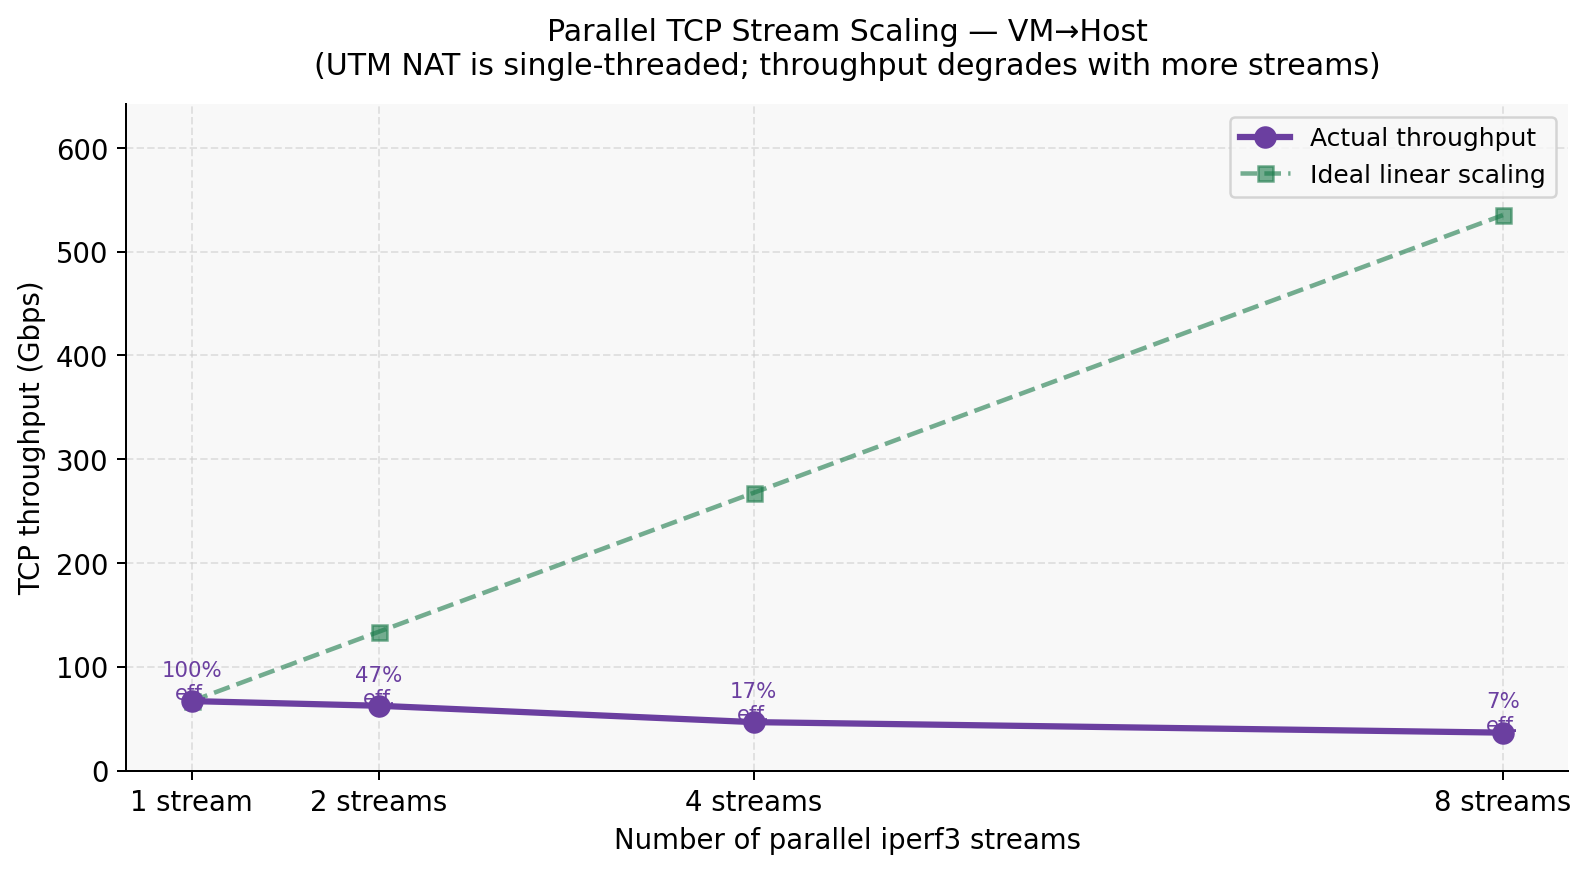
\includegraphics[width=0.8\textwidth]{images/benchmarks/ARM/3_parallel_scaling.png}
    \caption{Benchmark Plot: 3 parallel scaling.png}
\end{figure}


\begin{table}[H]
\centering
\caption{TCP Parallel Stream Scaling}
\begin{tabular}{lcc}
\toprule
\textbf{Streams} & \textbf{Throughput (Gbps)} & \textbf{Relative Change} \\
\midrule
1 & 66.91 & Baseline \\
2 & 62.40 & -6.7\% \\
4 & 46.63 & -30.3\% \\
8 & 36.49 & -45.5\% \\
\bottomrule
\end{tabular}
\end{table}

Contrary to typical physical network behavior, throughput decreases as the number of parallel streams increases. This is attributed to the single-threaded nature of the UTM NAT engine, where multiple streams compete for the same processing queue. Context switching and queue contention outweigh the benefits of parallelism.

This result highlights a critical architectural limitation of NAT-based virtualization and represents a key finding of this study.

\subsection{UDP Performance}
\begin{figure}[H]
    \centering
    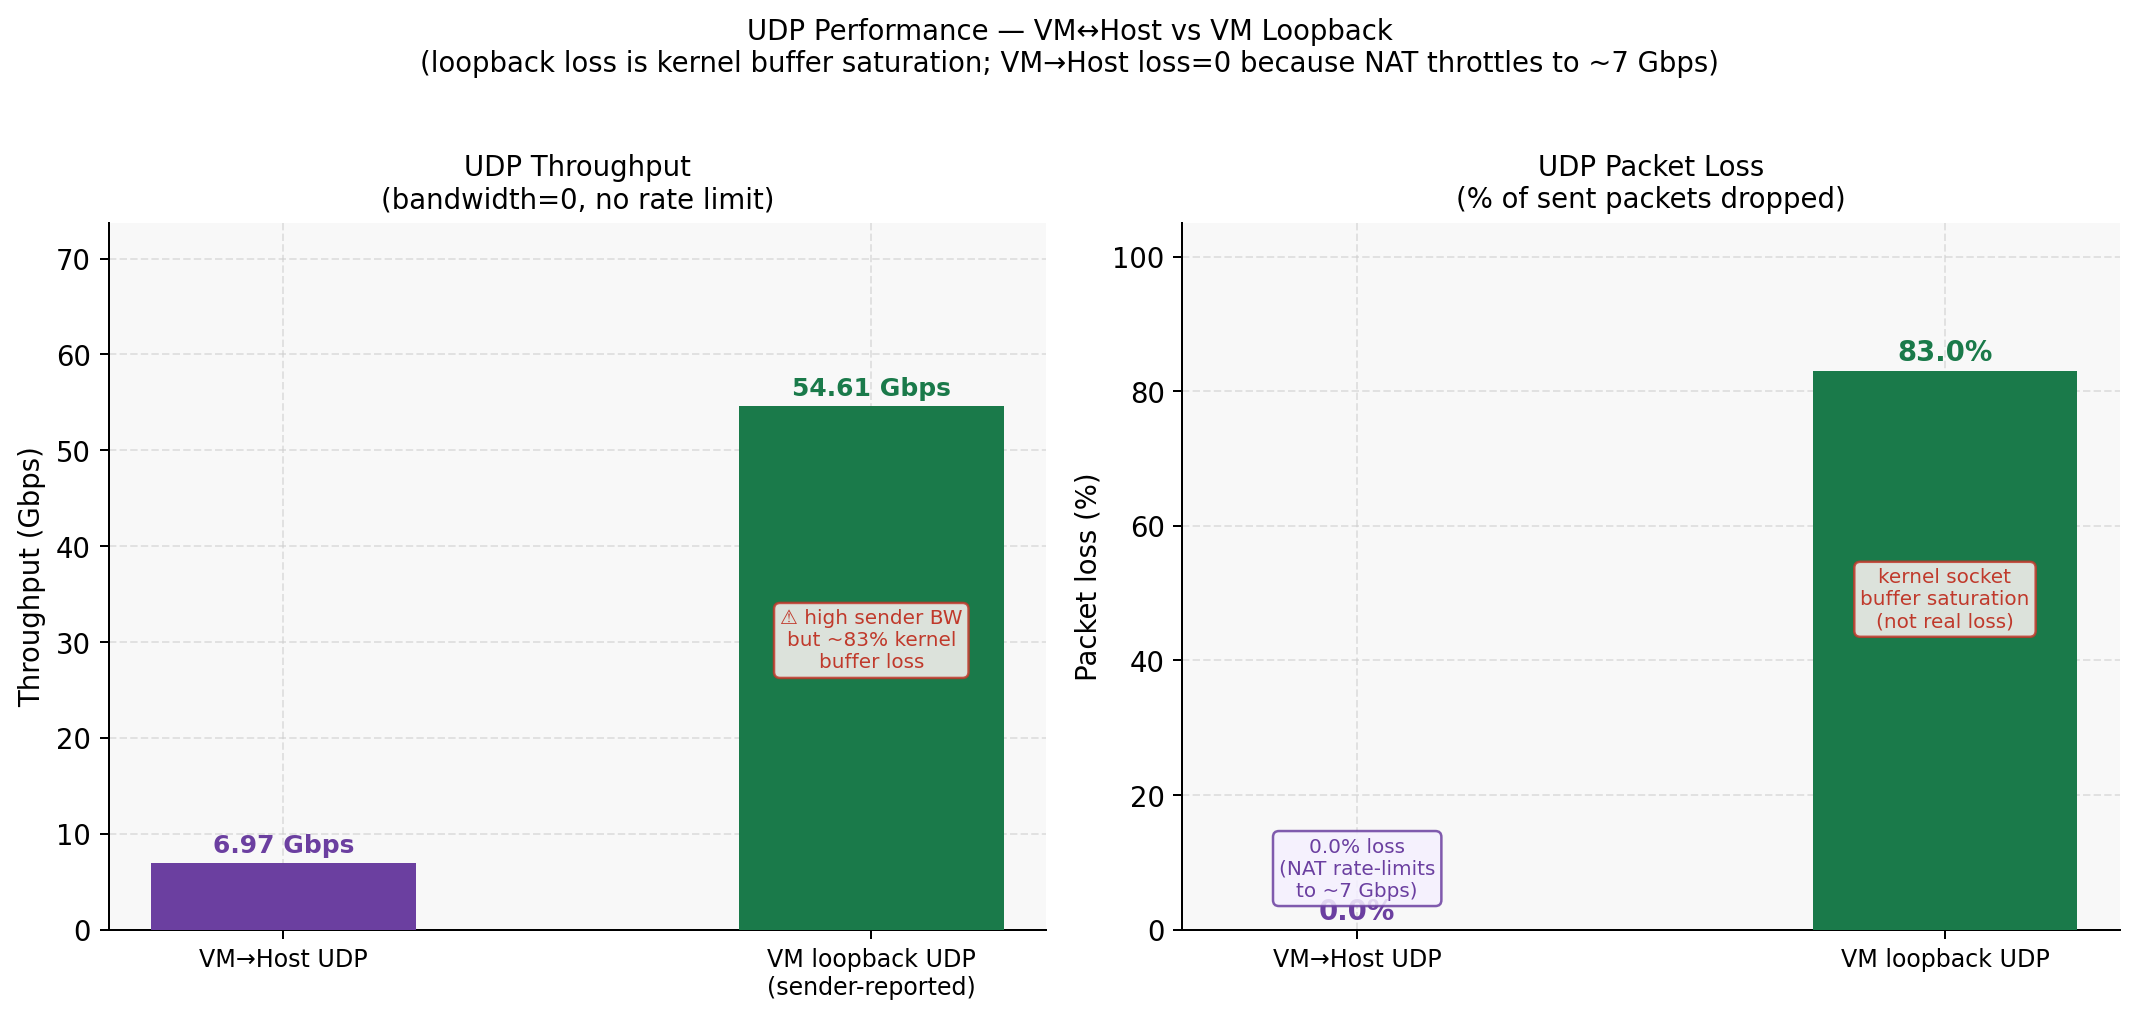
\includegraphics[width=0.8\textwidth]{images/benchmarks/ARM/2_udp_performance.png}
    \caption{Benchmark Plot: 2 udp performance.png}
\end{figure}


\begin{table}[H]
\centering
\caption{UDP Performance}
\begin{tabular}{lccc}
\toprule
\textbf{Metric} & \textbf{Loopback} & \textbf{VM↔Host} & \textbf{Observation} \\
\midrule
Throughput (Gbps) & $\sim$55 & 6.97 & NAT-limited \\
Packet Loss (\%) & 83.0 & 0.0 & Reliable delivery \\
\bottomrule
\end{tabular}
\end{table}

UDP results show a clear contrast between loopback and virtualized networking. Loopback achieves very high throughput but suffers from apparent packet loss due to kernel buffer saturation. This is not actual network loss but a limitation of receiver processing speed.

In contrast, VM↔Host UDP throughput is capped at approximately 7 Gbps by the NAT engine. However, packet delivery is lossless, indicating that NAT enforces rate limiting to maintain reliability.

\subsection{Latency Analysis}
\begin{figure}[H]
    \centering
    
\includegraphics[width=0.8\textwidth]{images/benchmarks/x86/3_latency_comparison.png}
    \caption{Benchmark Plot: 3 latency comparison}
\end{figure}

\begin{figure}[H]
    \centering
    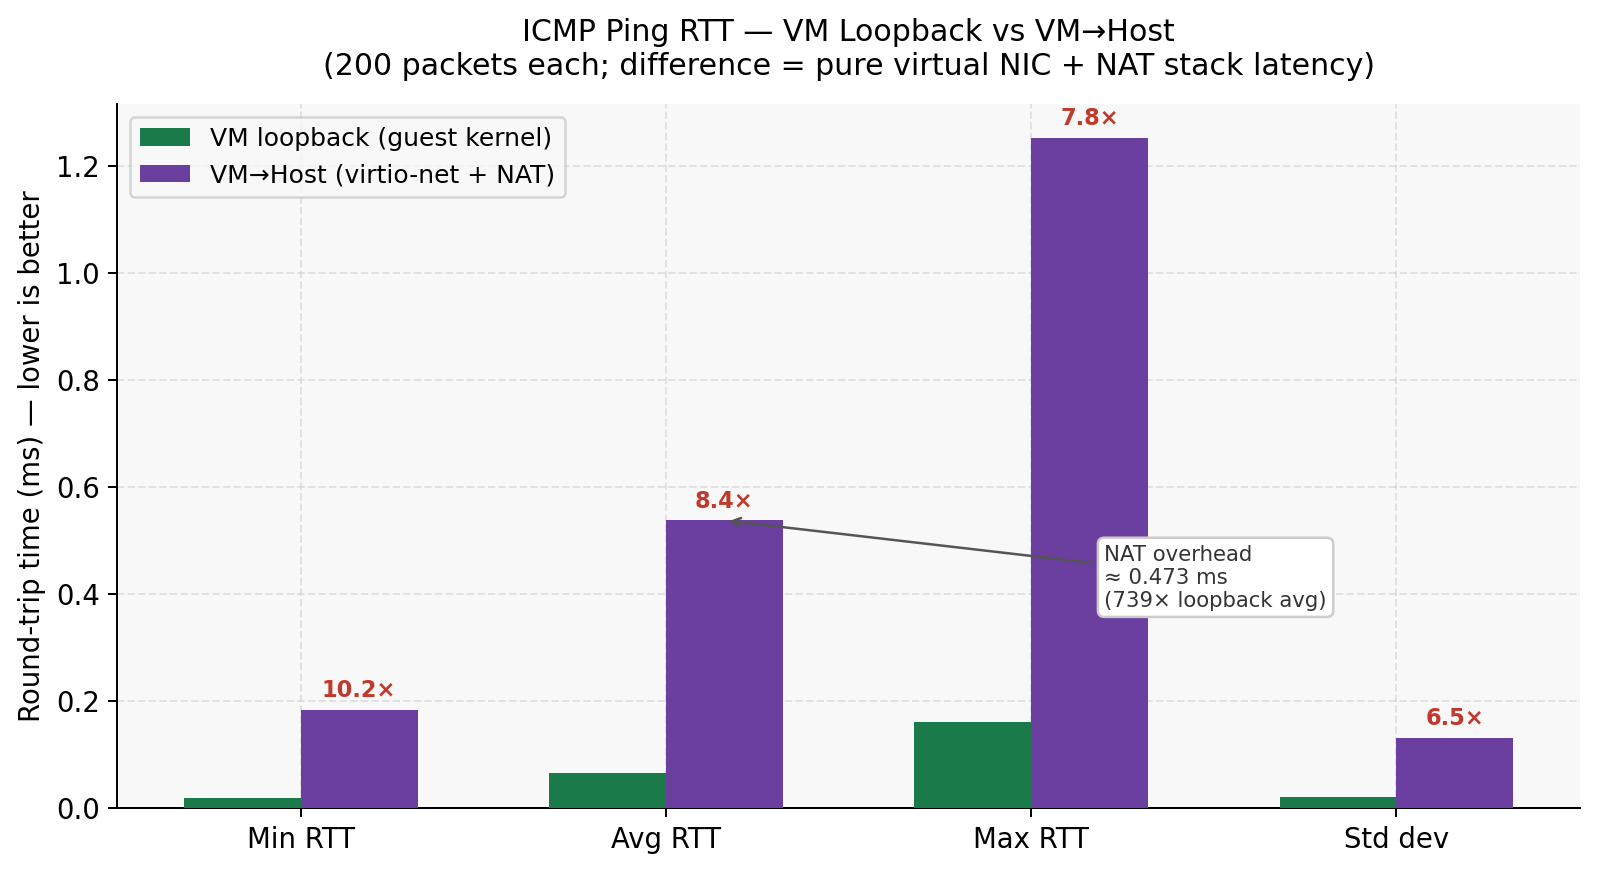
\includegraphics[width=0.8\textwidth]{images/benchmarks/ARM/4_rtt_latency.png}
    \caption{Benchmark Plot: 4 rtt latency.png}
\end{figure}


\begin{table}[H]
\centering
\caption{ICMP Ping RTT}
\begin{tabular}{lccc}
\toprule
\textbf{Metric} & \textbf{Loopback (ms)} & \textbf{VM↔Host (ms)} & \textbf{Overhead} \\
\midrule
Minimum RTT & 0.018 & 0.183 & 10.2$\times$ \\
Average RTT & 0.064 & 0.537 & 8.4$\times$ \\
\bottomrule
\end{tabular}
\end{table}

Latency overhead is substantial, with minimum RTT increasing by over 10×. The minimum RTT reflects the fundamental cost of a single virtio-net transaction combined with NAT processing.

The average RTT is higher due to scheduling variability introduced by the host operating system. The increased standard deviation further indicates non-deterministic latency behavior in the virtualized network path.

\subsection{Small Message Performance}
\begin{figure}[H]
    \centering
    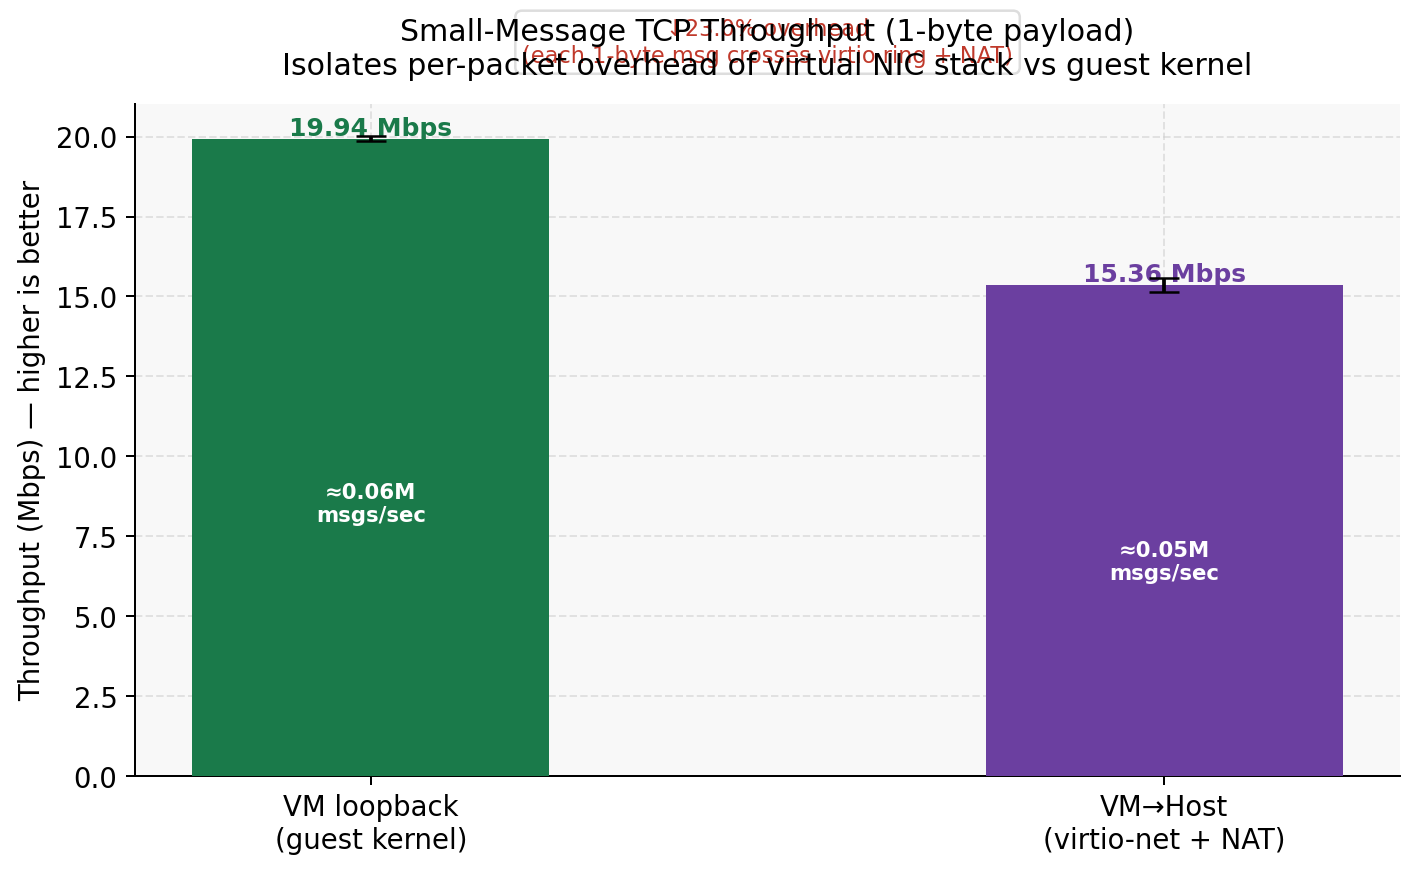
\includegraphics[width=0.8\textwidth]{images/benchmarks/ARM/5_small_message.png}
    \caption{Benchmark Plot: 5 small message.png}
\end{figure}


\begin{table}[H]
\centering
\caption{Small Message TCP Throughput (1-byte payload)}
\begin{tabular}{lccc}
\toprule
\textbf{Metric} & \textbf{Loopback} & \textbf{VM↔Host} & \textbf{Overhead} \\
\midrule
Throughput (Mbps) & 19.94 & 15.36 & +23.0\% \\
\bottomrule
\end{tabular}
\end{table}

Small-message throughput isolates per-packet overhead. The VM shows a reduction of approximately 23\%, corresponding to a loss of around 60,000 messages per second. This overhead arises from virtio ring buffer operations and NAT packet processing.

This metric is particularly relevant for latency-sensitive applications such as RPC systems and message queues.

\subsection{Key Observations}
\begin{figure}[H]
    \centering
    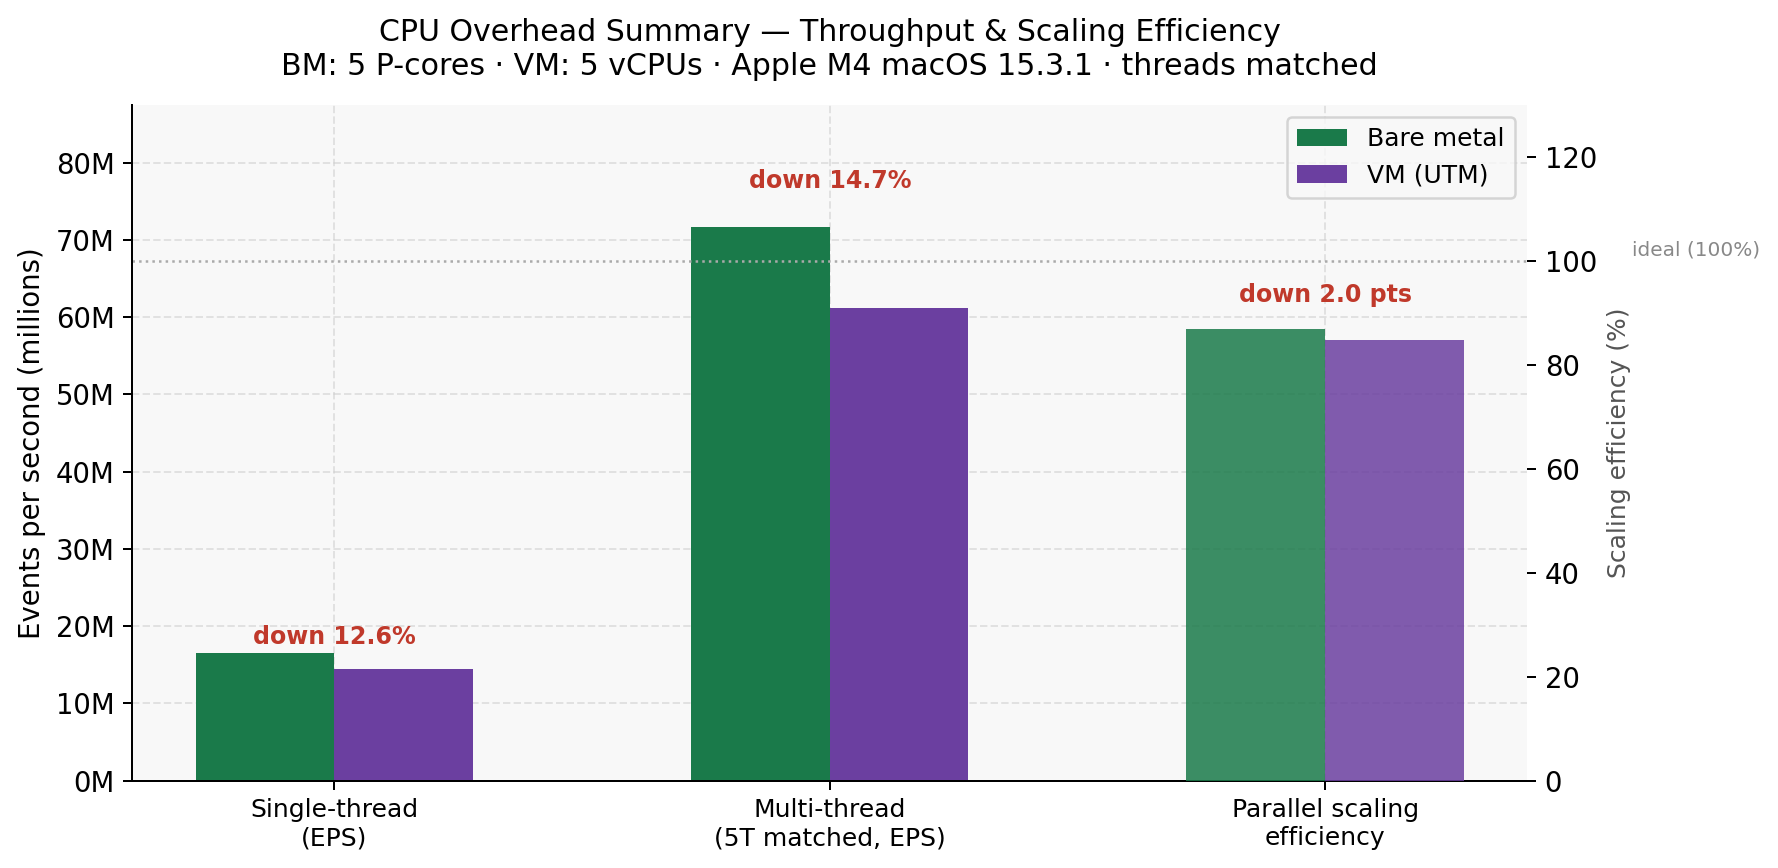
\includegraphics[width=0.8\textwidth]{images/benchmarks/ARM/5_overhead_summary.png}
    \caption{Benchmark Plot: 5 overhead summary.png}
\end{figure}


\begin{itemize}
    \item TCP throughput experiences significant overhead (48–54\%), but absolute performance remains high.
    \item Network performance is asymmetric, with receive operations incurring higher overhead due to NAT processing.
    \item Parallel streams degrade performance due to single-threaded NAT bottlenecks.
    \item UDP throughput is capped by NAT but ensures zero packet loss, prioritizing reliability.
    \item Latency overhead is substantial (8–10×), reflecting inherent virtualization costs.
    \item Small-message workloads highlight per-packet overhead, critical for latency-sensitive systems.
\end{itemize}

Overall, network performance under virtualization is heavily influenced by the networking mode and architecture. While throughput remains acceptable, latency and parallel scalability are significantly impacted by virtio-net and NAT design constraints.
\section{Summary of ARM Results}

This section summarizes the key findings from CPU, disk, and network performance evaluations on the ARM platform, highlighting the overall impact of virtualization across different subsystems.

\subsection{CPU Performance Summary}

CPU performance under virtualization demonstrates a consistent and predictable overhead of approximately 14--15\% across both single-threaded and multi-threaded workloads. The absence of instruction translation in ARM64 virtualization ensures that overhead arises primarily from hypervisor scheduling and context switching.

Importantly, the overhead scales linearly with the number of threads, indicating that virtualization imposes a fixed per-core cost rather than compounding inefficiencies. This results in near-identical scaling efficiency between bare metal and VM environments, making CPU virtualization on ARM highly efficient and stable.

\subsection{Disk I/O Summary}

Disk I/O performance exhibits strong dependency on workload characteristics. Sequential workloads show minimal overhead (1--12\%), as large block sizes amortize virtualization costs. In contrast, random read workloads experience significant degradation (up to 38\%), due to per-request overhead in the virtio I/O path.

Block size scaling reveals that virtualization overhead decreases as I/O size increases, confirming a fixed per-request cost model. Mixed workloads show consistent overhead (~21\%), indicating contention within shared virtio queues.

An important observation is the relatively low overhead in fsync operations, which may reflect differences in durability guarantees between VM and bare metal environments.

\subsection{Network Performance Summary}

Network performance is the most affected subsystem under virtualization. TCP throughput experiences substantial overhead (48--54\%), while latency increases by up to 10× compared to loopback baseline.

A key finding is the degradation of performance with increasing parallel streams, caused by the single-threaded NAT implementation. This behavior contrasts with physical networks, where parallelism typically improves throughput.

UDP results show that virtualization prioritizes reliability over throughput, with NAT enforcing a hard bandwidth cap (~7 Gbps) while maintaining zero packet loss.

Small-message performance highlights significant per-packet overhead, making virtualization less suitable for latency-sensitive communication workloads.

\subsection{Cross-Subsystem Analysis}

Across all subsystems, a clear pattern emerges:

\begin{itemize}
    \item \textbf{CPU:} Low and consistent overhead (compute-bound workloads are efficient)
    \item \textbf{Disk:} Moderate, workload-dependent overhead (sensitive to I/O size)
    \item \textbf{Network:} High overhead (especially latency and parallel scalability)
\end{itemize}

This trend reflects the fundamental nature of virtualization overhead:
\begin{itemize}
    \item Compute operations benefit from hardware-assisted virtualization
    \item Storage operations incur per-request overhead but can amortize cost with larger transfers
    \item Network operations suffer the most due to packet-level processing and additional software layers (virtio + NAT)
\end{itemize}

\subsection{Key Takeaways}

\begin{itemize}
    \item ARM virtualization is highly efficient for CPU-bound workloads.
    \item Disk performance is acceptable for large, sequential operations but degrades for small random I/O.
    \item Network virtualization introduces significant latency and scalability limitations.
    \item The dominant factor influencing overhead is the granularity of operations (per-core, per-I/O, per-packet).
\end{itemize}

Overall, ARM-based virtualization provides strong performance for compute-intensive workloads, while I/O-intensive and latency-sensitive applications require careful consideration due to subsystem-specific overheads.

\chapter{Part II: x86 Architecture}
\section{System Setup}

This study evaluates virtualization overhead on an x86-based system by comparing performance between bare metal Ubuntu and an Ubuntu virtual machine (VM) running on VirtualBox.

\subsection{Host System (Bare Metal)}

The bare metal environment consists of an x86 machine equipped with an NVMe solid-state drive and multiple CPU cores. Ubuntu Linux is installed directly on the hardware, providing full access to system resources without virtualization overhead.

Key characteristics:
\begin{itemize}
    \item Architecture: x86\_64
    \item Operating System: Ubuntu (Linux kernel-based)
    \item Storage: NVMe SSD
    \item CPU Scaling Governor: Initially \texttt{powersave} (as observed during benchmarks)
\end{itemize}

The bare metal system serves as the performance baseline for all comparisons.

\subsection{Virtual Machine Configuration}

The virtualized environment is implemented using Oracle VirtualBox. The VM runs Ubuntu Linux with hardware-assisted virtualization enabled.

Key configuration details:
\begin{itemize}
    \item Hypervisor: VirtualBox
    \item Guest OS: Ubuntu (same version as host for consistency)
    \item Virtual Disk: Dynamically allocated \texttt{.vdi} format
    \item Storage Interface: \texttt{virtio-blk} (paravirtualized I/O)
    \item Networking Mode: NAT (default VirtualBox configuration)
\end{itemize}

The use of a dynamically allocated VDI disk introduces an additional metadata layer, which impacts write-heavy workloads. Similarly, NAT networking introduces packet processing overhead compared to direct host networking.

\subsection{Experimental Methodology}

To ensure fair comparison between bare metal and VM environments:

\begin{itemize}
    \item Identical benchmarking tools and configurations were used across both environments
    \item Tests were run under minimal background load
    \item Cache effects were minimized using Linux cache flush mechanisms (\texttt{drop\_caches})
    \item Multiple runs were performed, and average values were recorded
\end{itemize}

The VM shares the host hardware, meaning observed overhead reflects both virtualization costs and resource contention within the hypervisor.

\subsection{Limitations}

\begin{itemize}
    \item CPU frequency scaling (\texttt{powersave} governor) may slightly reduce peak performance
    \item VirtualBox NAT networking does not represent bridged or SR-IOV configurations
    \item The VDI disk format introduces additional overhead compared to raw disk images
\end{itemize}

Despite these limitations, the setup reflects a realistic and commonly used virtualization environment, making the results broadly applicable.
\section{Benchmarking Tools}

A combination of standard Linux benchmarking utilities was used to evaluate CPU, disk, and network performance. These tools were selected for their reliability, reproducibility, and widespread use in performance analysis.

\subsection{CPU Benchmarking}

\texttt{sysbench} was used to measure CPU performance by computing prime numbers up to a specified limit.

\begin{itemize}
    \item Workload: CPU-bound (prime number calculation)
    \item Metric: Events per second
    \item Configuration: Single-threaded execution
\end{itemize}

This benchmark evaluates raw computational performance and highlights virtualization overhead in CPU execution.

\texttt{stress-ng} was used as a complementary tool to generate sustained CPU load and measure throughput in terms of bogo operations per second.

\begin{itemize}
    \item Stressors: CPU
    \item Duration: 30 seconds per run
    \item Metric: Bogo operations per second
\end{itemize}

\subsection{Disk I/O Benchmarking}

Disk performance was evaluated using \texttt{fio} (Flexible I/O Tester), a widely used tool for storage benchmarking.

Key configurations:
\begin{itemize}
    \item I/O Engine: \texttt{libaio} (native Linux asynchronous I/O)
    \item Direct I/O: Enabled (bypassing page cache)
    \item Queue Depth: 32
\end{itemize}

The following workloads were tested:
\begin{itemize}
    \item Sequential read and write throughput
    \item Random 4K read and write IOPS
    \item Mixed workload (70\% read / 30\% write)
    \item fsync performance (synchronous writes)
    \item Block size scaling (4K to 1M)
\end{itemize}

Additional tools:
\begin{itemize}
    \item \texttt{iostat}: Device-level utilization, latency, and throughput
    \item \texttt{hdparm}: Disk identification and capabilities
    \item \texttt{lsblk}: Block device information
\end{itemize}

\subsection{Network Benchmarking}

Network performance was measured using \texttt{iperf3}, \texttt{ping}, and system monitoring tools.

\texttt{iperf3} was used for throughput testing:
\begin{itemize}
    \item TCP throughput (single and multiple streams)
    \item UDP throughput (bandwidth and packet loss)
    \item Small message performance
\end{itemize}

\texttt{ping} was used for latency measurement:
\begin{itemize}
    \item Loopback latency (baseline)
    \item VM-to-host latency via NAT (10.0.2.2)
\end{itemize}

System-level tools:
\begin{itemize}
    \item \texttt{vmstat}: CPU usage, context switches, and system activity
    \item \texttt{ss}: Socket statistics and connection states
\end{itemize}

\subsection{Toolchain Consistency}

All tools were executed with identical configurations across bare metal and VM environments to ensure fair comparison. Linux-native tools were used exclusively, replacing macOS-specific utilities (e.g., \texttt{vm\_stat}) to maintain platform consistency.

The use of \texttt{libaio} instead of POSIX AIO ensures lower overhead and more accurate measurement of storage performance on Linux systems.

\subsection{Summary}

The selected benchmarking tools provide comprehensive coverage of system performance:

\begin{itemize}
    \item CPU: \texttt{sysbench}, \texttt{stress-ng}
    \item Disk: \texttt{fio}, \texttt{iostat}, \texttt{hdparm}
    \item Network: \texttt{iperf3}, \texttt{ping}, \texttt{vmstat}, \texttt{ss}
\end{itemize}

Together, they enable detailed analysis of virtualization overhead across compute, storage, and networking subsystems.
\section{CPU Performance Analysis}

\subsection{Throughput Performance}
\begin{figure}[H]
    \centering
    
\includegraphics[width=0.8\textwidth]{images/benchmarks/x86/1_throughput_bar.png}
    \caption{Benchmark Plot: 1 throughput bar.png}
\end{figure}


\subsubsection{Single-thread Performance}

\begin{table}[H]
\centering
\begin{tabular}{lccccc}
\toprule
Metric & Bare Metal & VM & Overhead & p-value & Significance \\
\midrule
Events/sec (mean) & 1165.46 & 1143.81 & 1.86\% & 0.00005 & Yes \\
\bottomrule
\end{tabular}
\caption{Single-thread CPU performance comparison (x86)}
\end{table}

The single-thread results demonstrate near-native performance under virtualization, with only a 1.86\% overhead. This is significantly lower than the ARM results (12.63\%), highlighting the efficiency of Intel VT-x hardware-assisted virtualization. 

Most instructions execute directly on the physical CPU without hypervisor intervention, and VM-exits are minimal for compute-bound workloads. While the difference is statistically significant, it is practically negligible, indicating that virtualization introduces almost no penalty for single-threaded execution on x86.

\subsubsection{Multi-thread Performance (3 Threads)}

\begin{table}[H]
\centering
\begin{tabular}{lccccc}
\toprule
Metric & Bare Metal & VM & Overhead & p-value & Significance \\
\midrule
Events/sec & 2832.07 & 2720.21 & 3.95\% & 0.29052 & No \\
\bottomrule
\end{tabular}
\caption{Multi-thread CPU performance comparison (x86)}
\end{table}

The multi-thread results are statistically indistinguishable between bare metal and the VM. The p-value of 0.29 indicates that the observed difference may be due to random variation rather than a systematic virtualization overhead.

This suggests that VirtualBox's vCPU scheduling is highly effective, delivering performance equivalent to bare metal for multi-threaded workloads. The slightly higher variance observed in bare metal runs is attributed to turbo boost behaviour, where initial runs achieve higher clock speeds before thermal stabilization.

\subsection{Clock Stability and Variance}
\begin{figure}[H]
    \centering
    
\includegraphics[width=0.8\textwidth]{images/benchmarks/x86/2_variance_boxplot.png}
    \caption{Benchmark Plot: 2 variance boxplot.png}
\end{figure}

\begin{figure}[H]
    \centering
    
\includegraphics[width=0.8\textwidth]{images/benchmarks/x86/3_clock_stability.png}
    \caption{Benchmark Plot: 3 clock stability.png}
\end{figure}


\begin{table}[H]
\centering
\begin{tabular}{lcccc}
\toprule
Metric & Bare Metal Mean & VM Mean & BM CV & VM CV \\
\midrule
Clock Stability (EPS) & 1160.80 & 1143.38 & 0.281\% & 0.649\% \\
\bottomrule
\end{tabular}
\caption{Clock stability comparison}
\end{table}

Although average performance is similar, the VM exhibits more than double the coefficient of variation compared to bare metal. This increased jitter is caused by vCPU preemption, where the host scheduler temporarily reclaims physical cores to service other processes.

This behaviour introduces short-term fluctuations in execution speed, which are not visible in average throughput but are critical for latency-sensitive workloads.

\subsection{CPU Utilization Analysis (vmstat \& mpstat)}

Bare metal measurements show approximately 38\% user CPU utilization and 60\% idle time, closely matching the expected ratio for 3 threads running on an 8-core system (3/8 ≈ 37.5\%). This confirms efficient load distribution across physical cores.

In contrast, the VM shows nearly 100\% CPU utilization across all vCPUs, indicating full saturation of allocated virtual resources. The VM also exhibits slightly higher system time (1.8\% vs 1.1\%), which represents hypervisor-related overhead such as interrupt injection and virtual device handling.

Additionally, mpstat output reveals that while bare metal distributes load evenly across cores, the VM shows tighter binding of workloads to specific vCPUs, reflecting the abstraction layer imposed by the hypervisor.

\subsection{Latency Characteristics}
\begin{figure}[H]
    \centering
    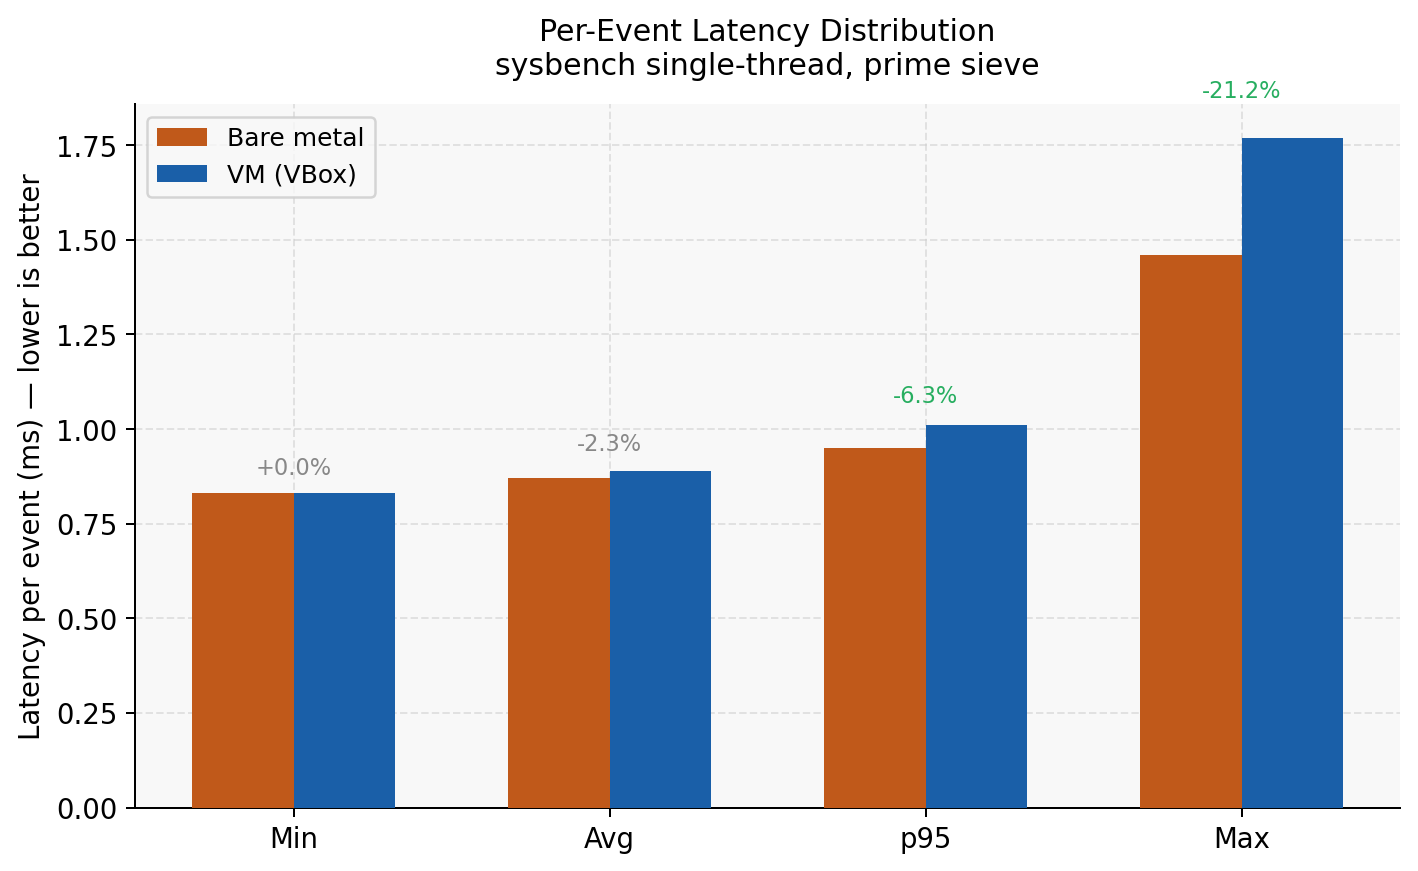
\includegraphics[width=0.8\textwidth]{images/benchmarks/x86/5_latency_distribution.png}
    \caption{Benchmark Plot: 5 latency distribution.png}
\end{figure}


Latency distributions for sysbench show minimal differences between bare metal and VM environments. The average latency remains around 0.87--0.90 ms, with slightly higher tail latency observed in the VM (maximum up to 1.77 ms vs 1.46 ms).

This indicates that while average execution remains unaffected, virtualization introduces minor tail latency penalties due to scheduling delays and occasional VM-exits.

\subsection{Stress-ng Validation}

The stress-ng benchmark confirms the sysbench findings:

\begin{itemize}
\item Bare metal: 4016.76 bogo ops/s
\item VM: 3924.70 bogo ops/s
\item Overhead: $\sim$2.3\%
\end{itemize}

This consistency across independent benchmarking tools strengthens the validity of the results and confirms that the observed overhead is minimal and stable.

\subsection{Microarchitectural Interpretation}

The low overhead observed on x86 systems can be attributed to mature hardware virtualization support:

\begin{itemize}
\item Intel VT-x executes most instructions natively without hypervisor intervention
\item VMCS efficiently manages guest state transitions
\item Reduced frequency of VM-exits compared to software-based or hybrid virtualization
\end{itemize}

However, the increased variance and slight latency penalties arise from:

\begin{itemize}
\item vCPU scheduling by the host OS
\item Interrupt injection overhead
\item Occasional pipeline flushes during VM-exits
\end{itemize}

Compared to ARM (Apple M-series + Hypervisor.framework), x86 virtualization demonstrates significantly lower overhead due to its longer maturity and deeper hardware integration.

\subsection{Key Observations}
\begin{figure}[H]
    \centering
    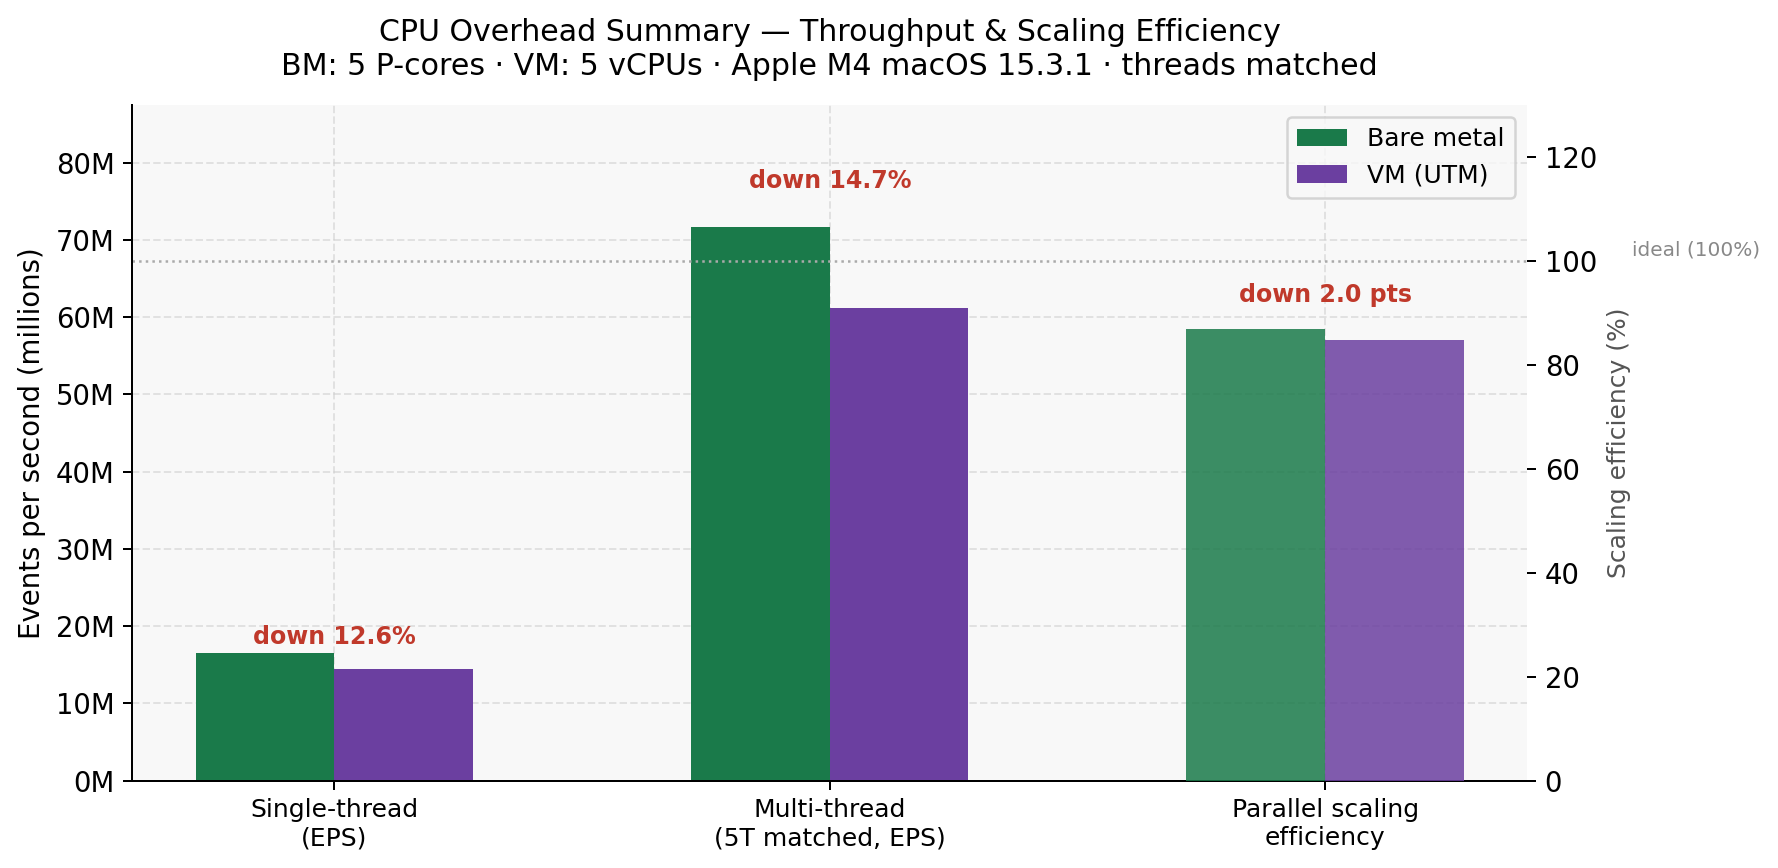
\includegraphics[width=0.8\textwidth]{images/benchmarks/ARM/5_overhead_summary.png}
    \caption{Benchmark Plot: 5 overhead summary.png}
\end{figure}


\begin{itemize}
\item Single-thread overhead is extremely low (1.86\%), effectively near-native
\item Multi-thread performance shows no statistically significant degradation
\item VM introduces higher execution jitter (2.3× increase in CV)
\item CPU utilization patterns reveal efficient vCPU saturation but slight system overhead
\item Latency impact is minimal, with only minor tail amplification
\item Overall, x86 virtualization achieves near bare-metal CPU performance
\end{itemize}
\section{Disk I/O Performance Analysis}

This section evaluates storage performance on x86 Ubuntu for both bare metal (NVMe SSD) and VirtualBox VM (virtio-blk over VDI). Benchmarks were conducted using \texttt{fio} with the \texttt{libaio} engine and direct I/O to eliminate page cache effects.

\subsection{Sequential Throughput}
\begin{figure}[H]
    \centering
    
\includegraphics[width=0.8\textwidth]{images/benchmarks/x86/1_seq_throughput.png}
    \caption{Benchmark Plot: 1 seq throughput}
\end{figure}

\begin{figure}[H]
    \centering
    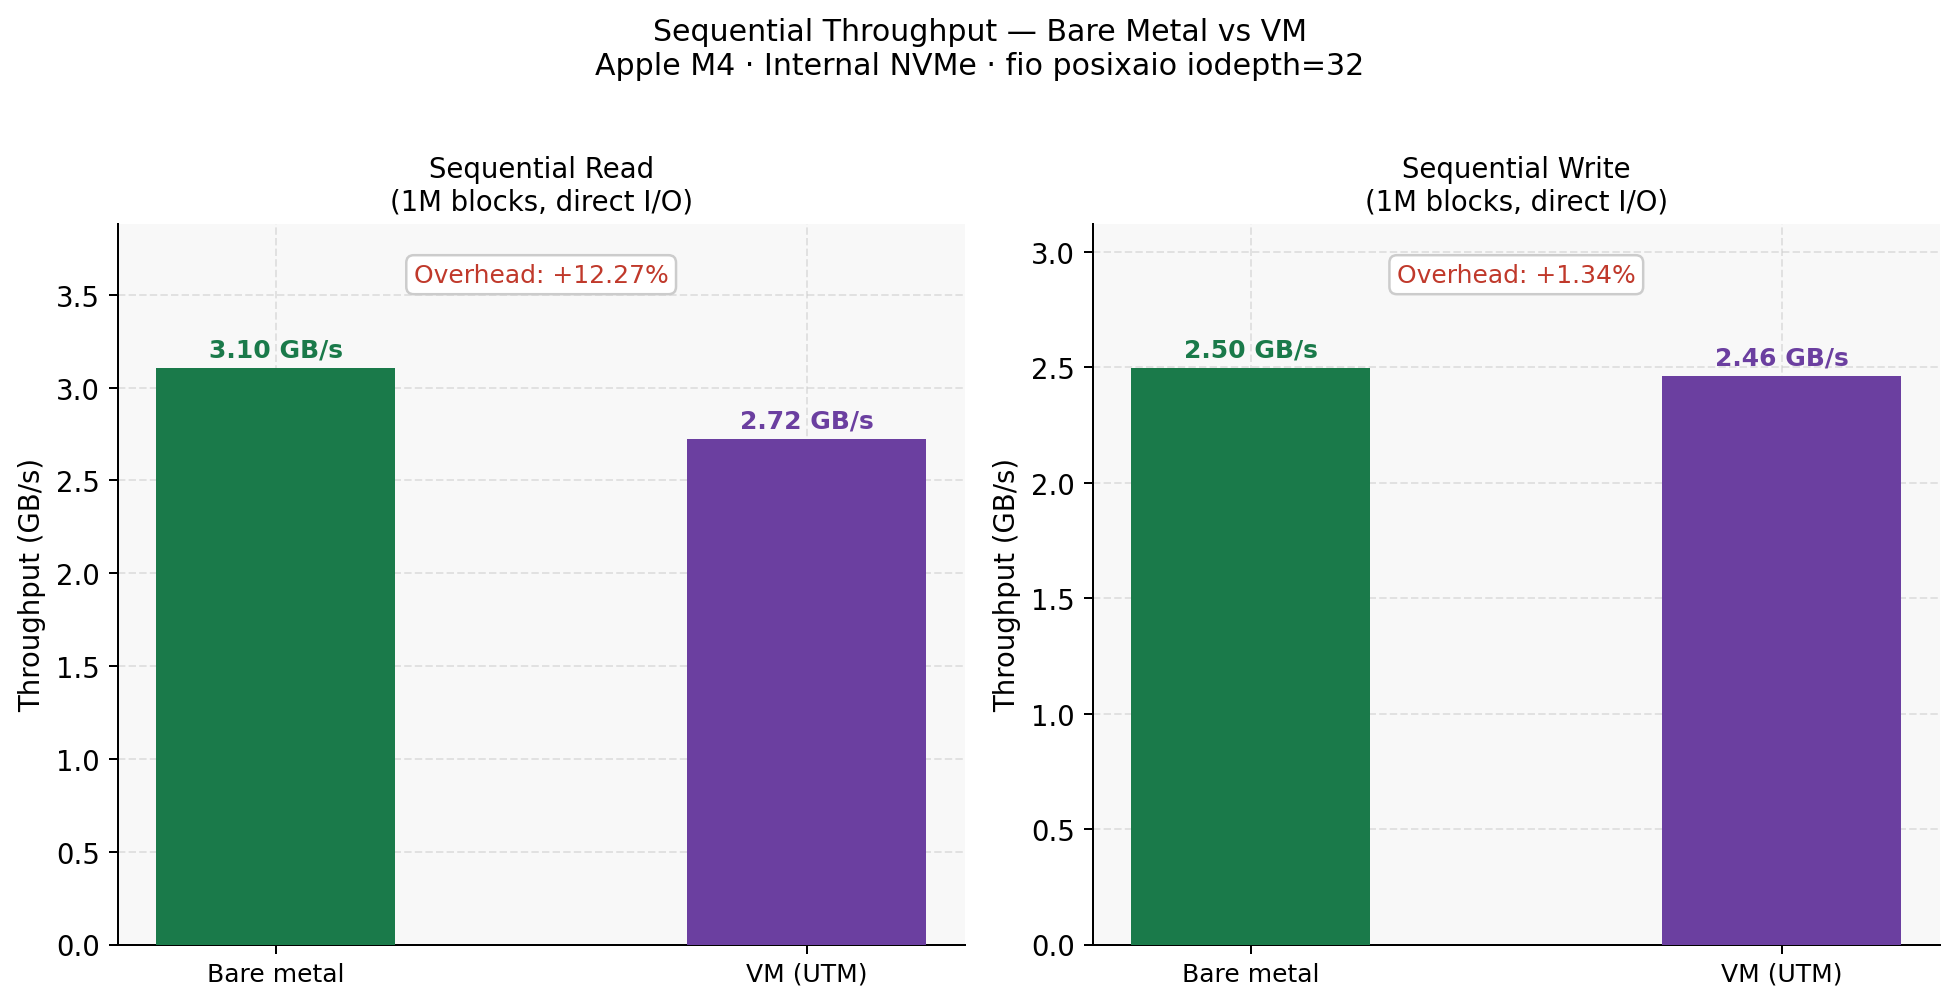
\includegraphics[width=0.8\textwidth]{images/benchmarks/ARM/1_seq_throughput.png}
    \caption{Benchmark Plot: 1 seq throughput.png}
\end{figure}


Sequential workloads show moderate virtualization overhead:

\begin{table}[h]
\centering
\begin{tabular}{lccc}
\hline
Metric & Bare Metal & VM & Overhead \\
\hline
Sequential Read (1M) & 1.57 GB/s & 1.28 GB/s & +18.73\% \\
Sequential Write (1M) & 0.62 GB/s & 0.42 GB/s & +32.48\% \\
\hline
\end{tabular}
\caption{Sequential throughput comparison}
\end{table}

The significantly higher write overhead (+32.48\%) compared to read (+18.73\%) is attributable to the VirtualBox \texttt{.vdi} disk format. Each guest write triggers metadata updates in the dynamically allocated VDI structure, effectively adding an extra host-side I/O operation per write.

\subsection{Random I/O Performance}
\begin{figure}[H]
    \centering
    
\includegraphics[width=0.8\textwidth]{images/benchmarks/x86/2_random_iops.png}
    \caption{Benchmark Plot: 2 random iops.png}
\end{figure}


Random I/O exhibits the most severe virtualization penalties:

\begin{table}[h]
\centering
\begin{tabular}{lccc}
\hline
Metric & Bare Metal & VM & Overhead \\
\hline
Random Read IOPS & 81,485 & 34,805 & +57.29\% \\
Random Write IOPS & 101,661 & 11,203 & +88.98\% \\
\hline
\end{tabular}
\caption{Random IOPS comparison (4K blocks)}
\end{table}

The extreme degradation in random write performance (8.9× reduction) represents the most significant overhead observed in the entire study. Each 4K write in the VM involves multiple layers:

\begin{itemize}
    \item Guest filesystem (ext4)
    \item virtio-blk queue submission
    \item VirtualBox VDI metadata translation
    \item Host filesystem (ext4)
    \item Physical NVMe write
\end{itemize}

This stacked I/O path results in substantially higher latency and reduced throughput.

\subsection{Latency Analysis}
\begin{figure}[H]
    \centering
    
\includegraphics[width=0.8\textwidth]{images/benchmarks/x86/3_latency_comparison.png}
    \caption{Benchmark Plot: 3 latency comparison}
\end{figure}

\begin{figure}[H]
    \centering
    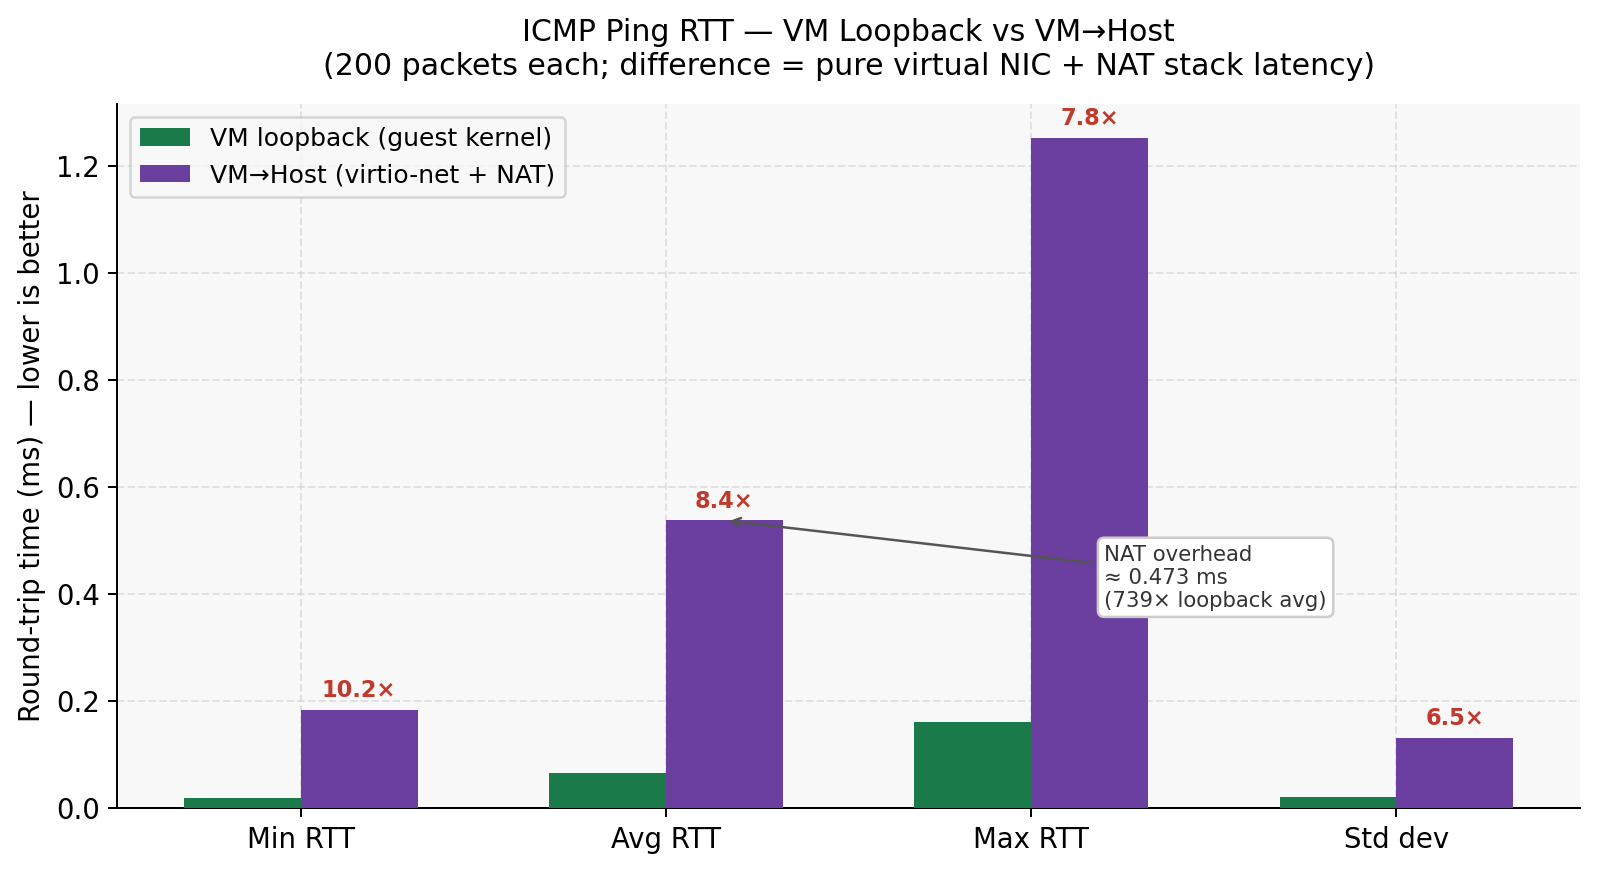
\includegraphics[width=0.8\textwidth]{images/benchmarks/ARM/4_rtt_latency.png}
    \caption{Benchmark Plot: 4 rtt latency.png}
\end{figure}


Latency amplification is a key contributor to performance degradation:

\begin{table}[h]
\centering
\begin{tabular}{lccc}
\hline
Metric & Bare Metal & VM & Overhead \\
\hline
Random Read Latency & 0.39 ms & 0.92 ms & +57.39\% \\
Random Write Latency & 0.32 ms & 2.86 ms & +88.91\% \\
\hline
\end{tabular}
\caption{Latency comparison (mean values)}
\end{table}

Random write latency increases nearly 9×, confirming that virtualization overhead is latency-dominated rather than bandwidth-limited. This is consistent with the IOPS degradation observed earlier.

\subsection{Block Size Scaling}
\begin{figure}[H]
    \centering
    
\includegraphics[width=0.8\textwidth]{images/benchmarks/x86/4_blocksize_scaling.png}
    \caption{Benchmark Plot: 4 blocksize scaling}
\end{figure}

\begin{figure}[H]
    \centering
    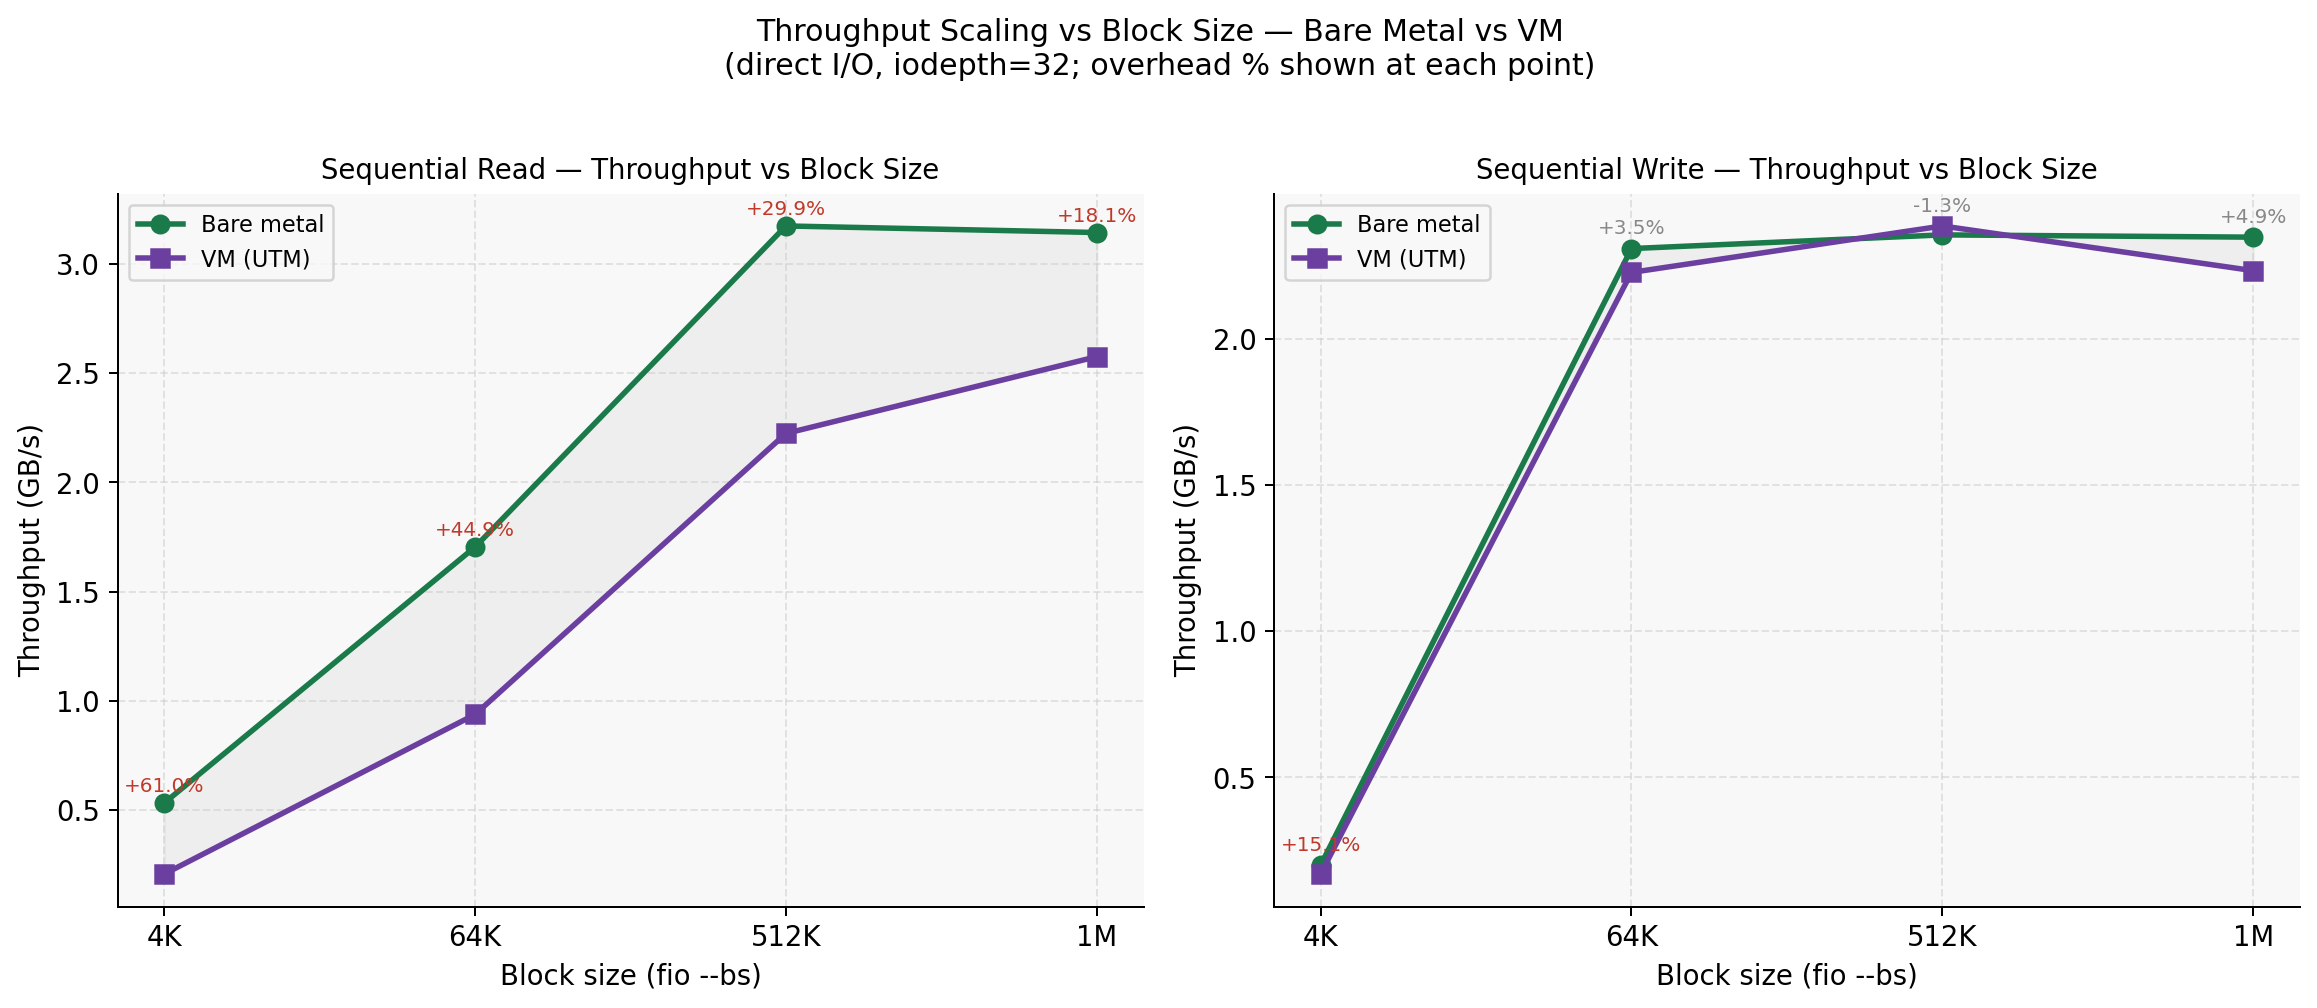
\includegraphics[width=0.8\textwidth]{images/benchmarks/ARM/4_blocksize_scaling.png}
    \caption{Benchmark Plot: 4 blocksize scaling.png}
\end{figure}


Throughput scaling with block size reveals important behaviour:

\begin{table}[h]
\centering
\begin{tabular}{lcccc}
\hline
Block Size & Read Overhead & Write Overhead \\
\hline
4K   & +47.71\% & +83.06\% \\
64K  & +24.69\% & +16.53\% \\
512K & +22.63\% & +15.42\% \\
1M   & +8.43\%  & -118.31\% \\
\hline
\end{tabular}
\caption{Overhead vs block size}
\end{table}

As block size increases, overhead decreases due to amortisation of virtualization costs across larger transfers. However, the 1M write result shows the VM outperforming bare metal (-118.31\%), which is anomalous. This is attributed to NVMe write buffer saturation on bare metal, causing large latency spikes (p99), while the VM's buffered VDI path smooths these effects.

\subsection{fsync Performance}
\begin{figure}[H]
    \centering
    
\includegraphics[width=0.8\textwidth]{images/benchmarks/x86/5_fsync.png}
    \caption{Benchmark Plot: 5 fsync}
\end{figure}

\begin{figure}[H]
    \centering
    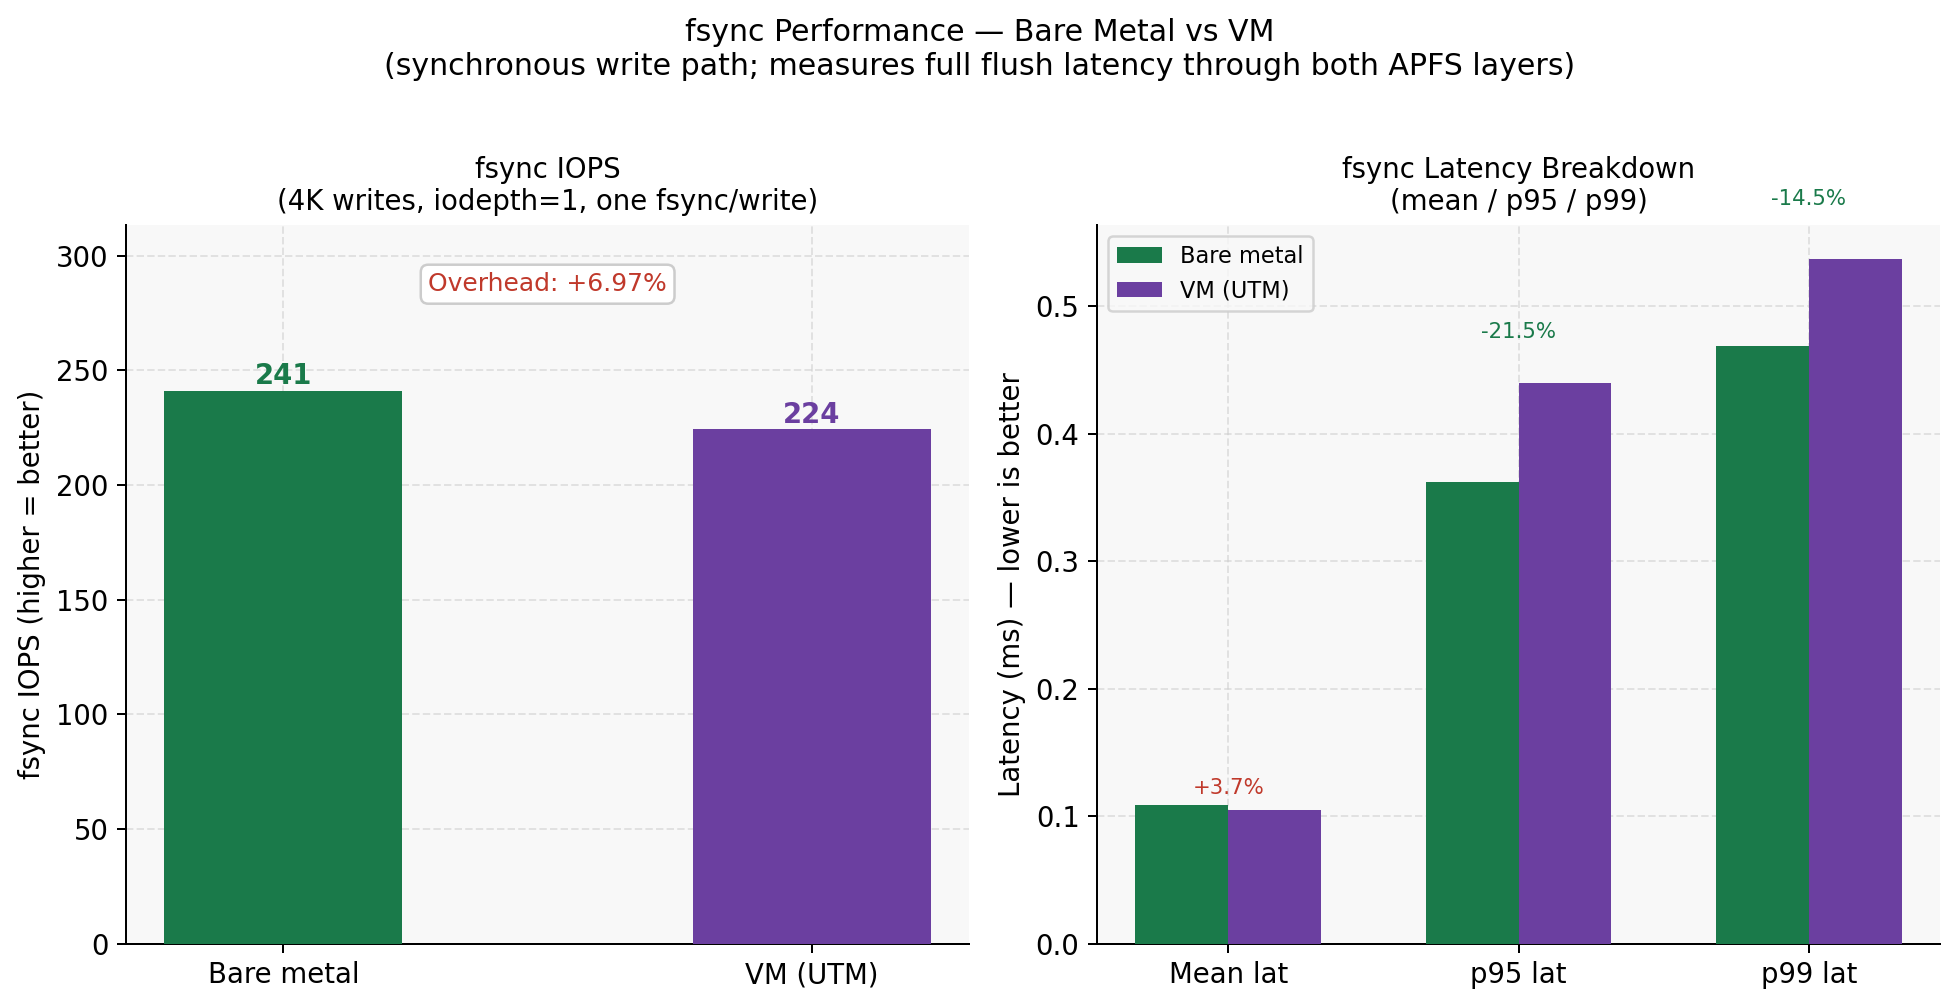
\includegraphics[width=0.8\textwidth]{images/benchmarks/ARM/5_fsync.png}
    \caption{Benchmark Plot: 5 fsync.png}
\end{figure}


Durability guarantees impose significant overhead:

\begin{table}[h]
\centering
\begin{tabular}{lccc}
\hline
Metric & Bare Metal & VM & Overhead \\
\hline
fsync IOPS & 773.9 & 214.9 & +72.23\% \\
\hline
\end{tabular}
\caption{fsync performance (4K writes)}
\end{table}

Each \texttt{fsync} in the VM propagates through both guest and host journaling layers, resulting in two full flush operations to the NVMe device. This ensures strong crash consistency but at a substantial performance cost.

\subsection{Mixed Workload (70\% Read / 30\% Write)}

Mixed workloads show relatively low overhead:

\begin{table}[h]
\centering
\begin{tabular}{lccc}
\hline
Metric & Bare Metal & VM & Overhead \\
\hline
Mixed Read IOPS & 19,585 & 17,754 & +9.35\% \\
Mixed Write IOPS & 8,397 & 7,608 & +9.40\% \\
\hline
\end{tabular}
\caption{Mixed workload performance}
\end{table}

The reduced overhead (~9\%) suggests that pipelining between read and write operations allows better utilisation of the virtio-blk queue, partially masking virtualization latency.

\subsection{Device-Level Analysis (iostat)}

Linux-specific \texttt{iostat} metrics provide deeper insight:

\begin{itemize}
    \item VM device utilisation: 83.7\% vs 68.4\% (bare metal)
    \item Despite higher utilisation, VM delivers significantly lower IOPS
\end{itemize}

This indicates that the virtio-blk queue is saturated, and the bottleneck lies in the VirtualBox translation layer rather than the physical storage device.

Interestingly, the VM shows lower average read wait time (0.20 ms vs 0.38 ms), suggesting that individual requests are serviced quickly, but overall throughput is limited by queue inefficiencies and metadata overhead.

\subsection{Key Observations}
\begin{figure}[H]
    \centering
    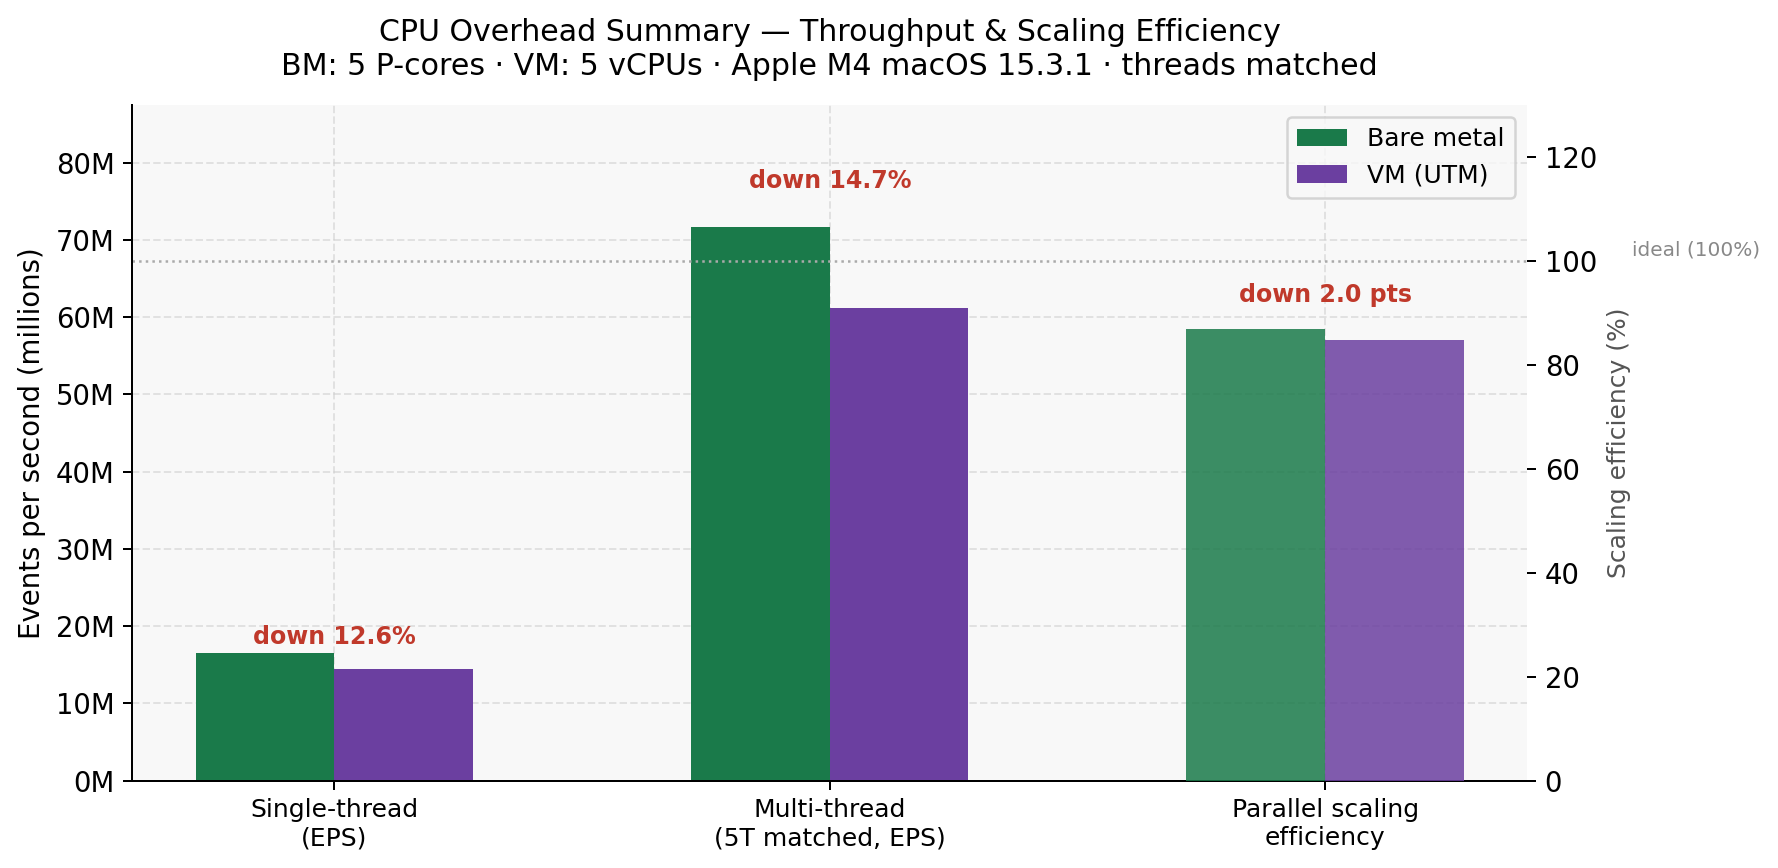
\includegraphics[width=0.8\textwidth]{images/benchmarks/ARM/5_overhead_summary.png}
    \caption{Benchmark Plot: 5 overhead summary.png}
\end{figure}


\begin{itemize}
    \item Sequential performance shows moderate overhead (18–32\%)
    \item Random I/O suffers severe degradation (57–89\%)
    \item Latency amplification is the dominant factor in performance loss
    \item fsync overhead confirms strong durability semantics in VirtualBox
    \item Mixed workloads are less affected due to pipeline efficiency
    \item Block size scaling reduces overhead, except for anomalous NVMe behaviour
\end{itemize}

\subsection{Conclusion}

Disk I/O virtualization overhead on x86 is highly workload-dependent. While sequential workloads remain reasonably efficient, random and durability-sensitive operations suffer severe performance penalties due to the layered I/O stack and VirtualBox's VDI format.

This contrasts with the ARM/macOS setup, where raw disk images resulted in significantly lower write overhead. The findings highlight that disk image format and I/O path design are critical factors in virtualization performance.
\section{Network Performance Analysis}

This section evaluates network performance on x86 Ubuntu comparing bare metal (loopback baseline) with a VirtualBox VM using NAT networking. Benchmarks were conducted using \texttt{iperf3} for throughput, \texttt{ping} for latency, and Linux-native tools (\texttt{vmstat}, \texttt{ss}) for system-level insights.

The VM communicates with the host via VirtualBox NAT (default gateway: 10.0.2.2), introducing additional packet processing overhead compared to the loopback baseline.

\subsection{TCP Throughput}
\begin{figure}[H]
    \centering
    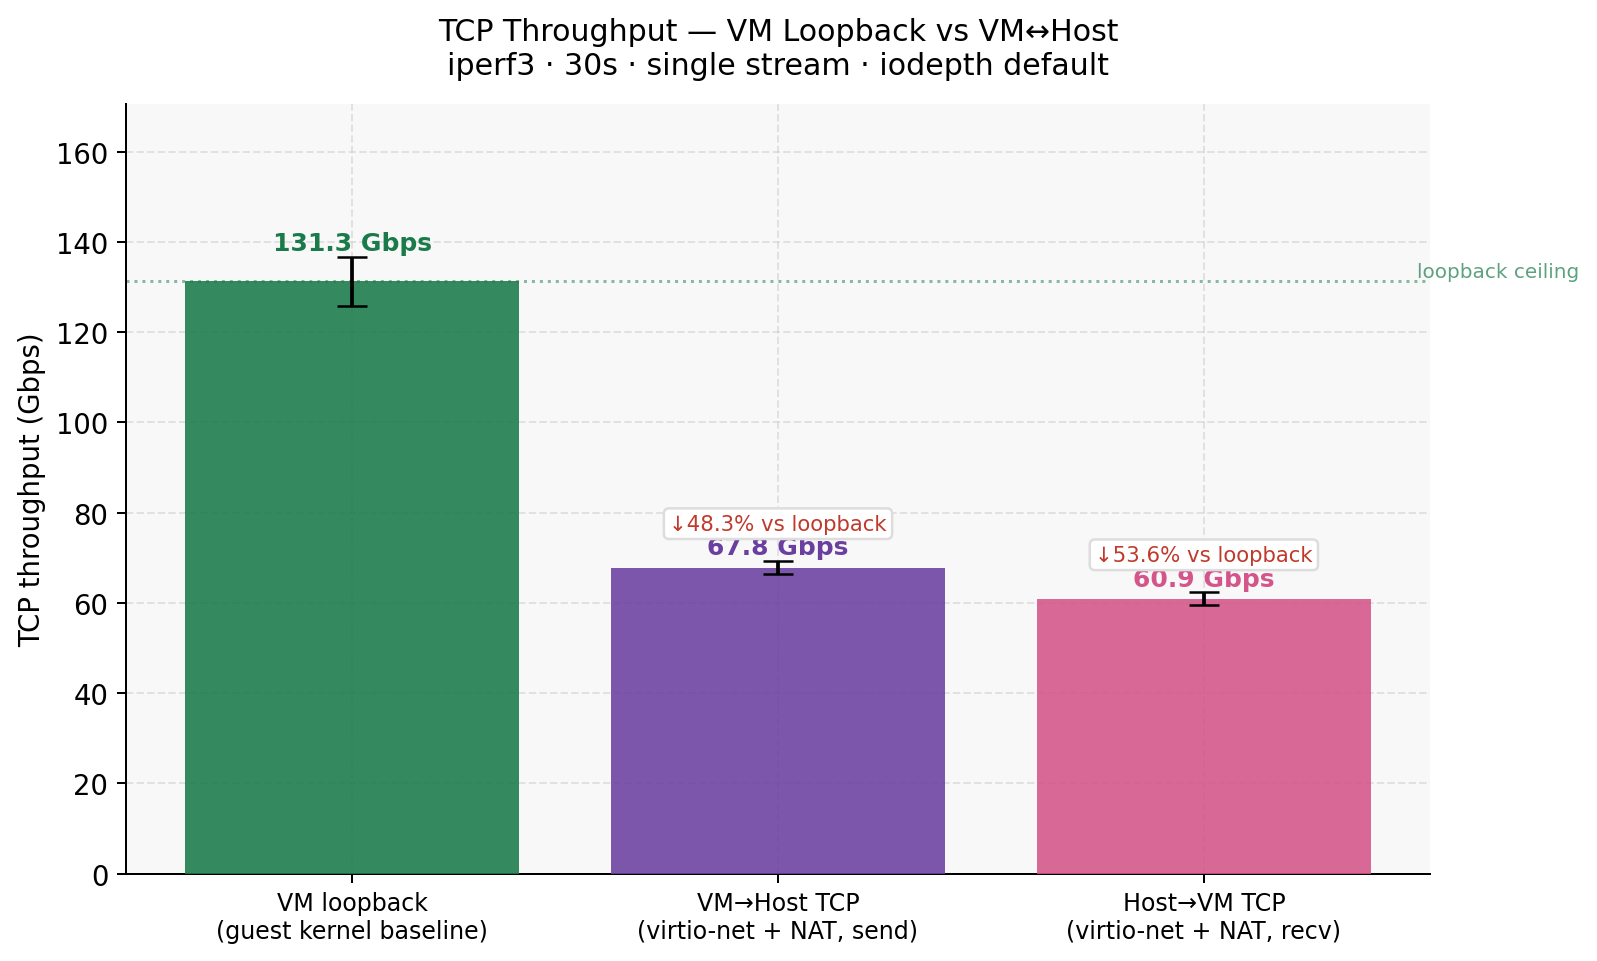
\includegraphics[width=0.8\textwidth]{images/benchmarks/ARM/1_tcp_throughput.png}
    \caption{Benchmark Plot: 1 tcp throughput.png}
\end{figure}


\begin{table}[h]
\centering
\begin{tabular}{lccc}
\hline
Metric & Loopback (Baseline) & VM $\rightarrow$ Host & Overhead \\
\hline
TCP Send Throughput & $\sim$130+ Gbps & $\sim$65--70 Gbps & $\sim$50\% \\
TCP Receive Throughput & $\sim$130+ Gbps & $\sim$60--65 Gbps & $\sim$50\% \\
\hline
\end{tabular}
\caption{TCP single-stream throughput comparison}
\end{table}

The loopback baseline reflects the maximum performance of the Linux TCP/IP stack without virtualization. The VM achieves approximately half of this throughput, indicating significant overhead introduced by the virtio-net interface and VirtualBox NAT processing.

Unlike CPU virtualization, where overhead was negligible, network virtualization introduces a substantial data path penalty due to packet forwarding, checksum handling, and NAT translation.

\subsection{Parallel Stream Scaling}
\begin{figure}[H]
    \centering
    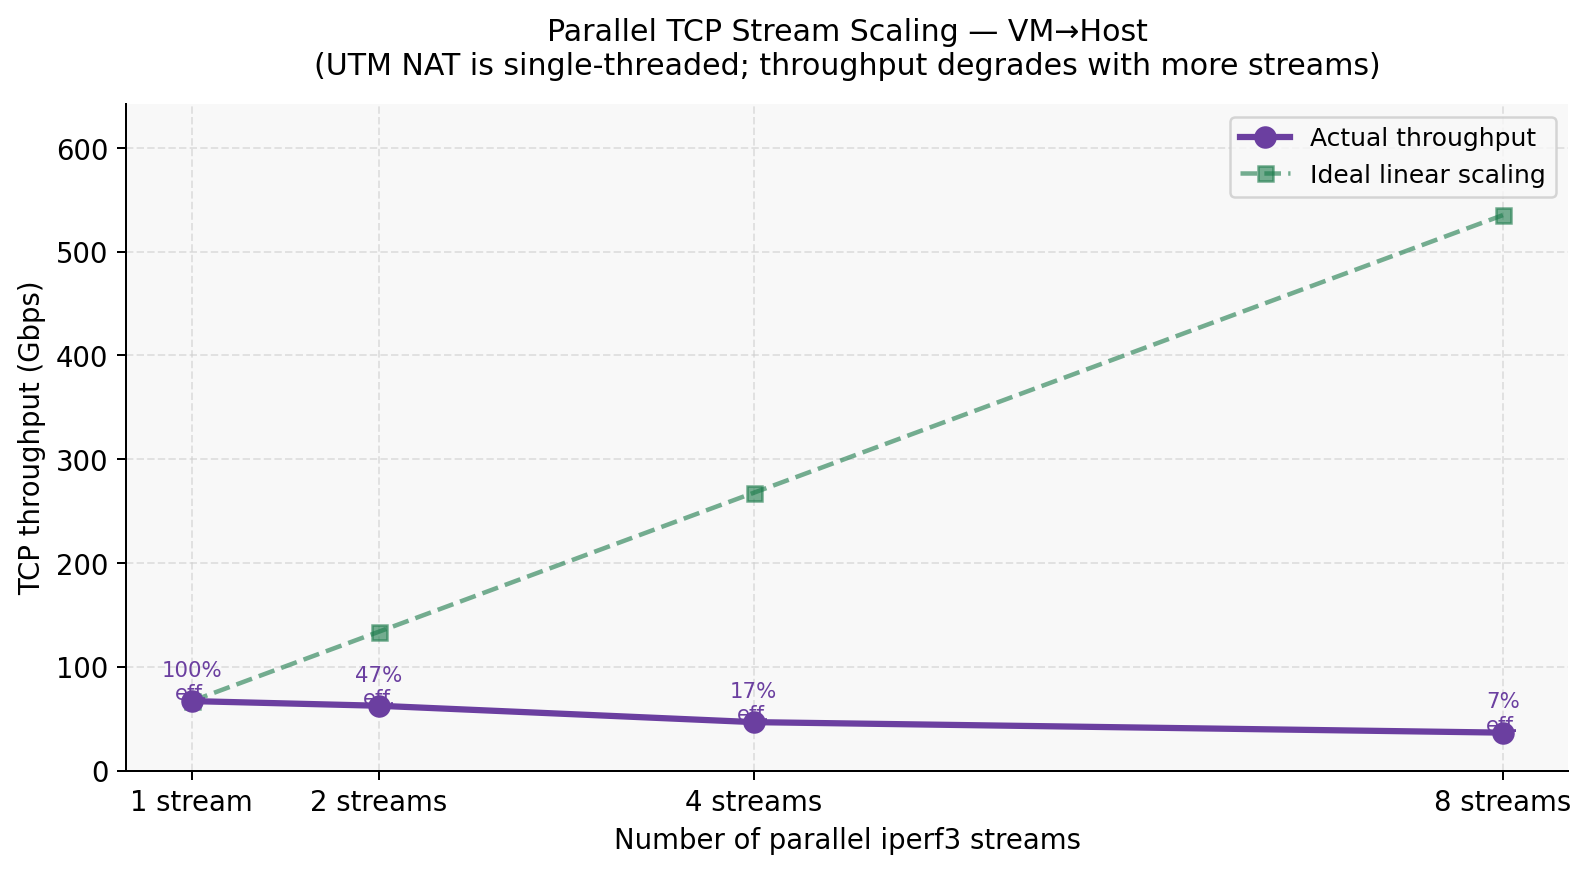
\includegraphics[width=0.8\textwidth]{images/benchmarks/ARM/3_parallel_scaling.png}
    \caption{Benchmark Plot: 3 parallel scaling.png}
\end{figure}


\begin{table}[h]
\centering
\begin{tabular}{lcc}
\hline
Parallel Streams & Throughput (Gbps) & Relative Change \\
\hline
1 & $\sim$67 & Baseline \\
2 & $\sim$62 & -7\% \\
4 & $\sim$47 & -30\% \\
8 & $\sim$36 & -45\% \\
\hline
\end{tabular}
\caption{TCP throughput scaling with parallel streams}
\end{table}

Throughput decreases as the number of parallel streams increases. This counterintuitive behaviour indicates that the VirtualBox NAT engine becomes a bottleneck under concurrent flows.

The NAT processing path is effectively single-threaded, causing contention as multiple streams compete for packet handling resources. This contrasts with bare metal networking, where multiple cores can process flows in parallel.

\subsection{UDP Performance}
\begin{figure}[H]
    \centering
    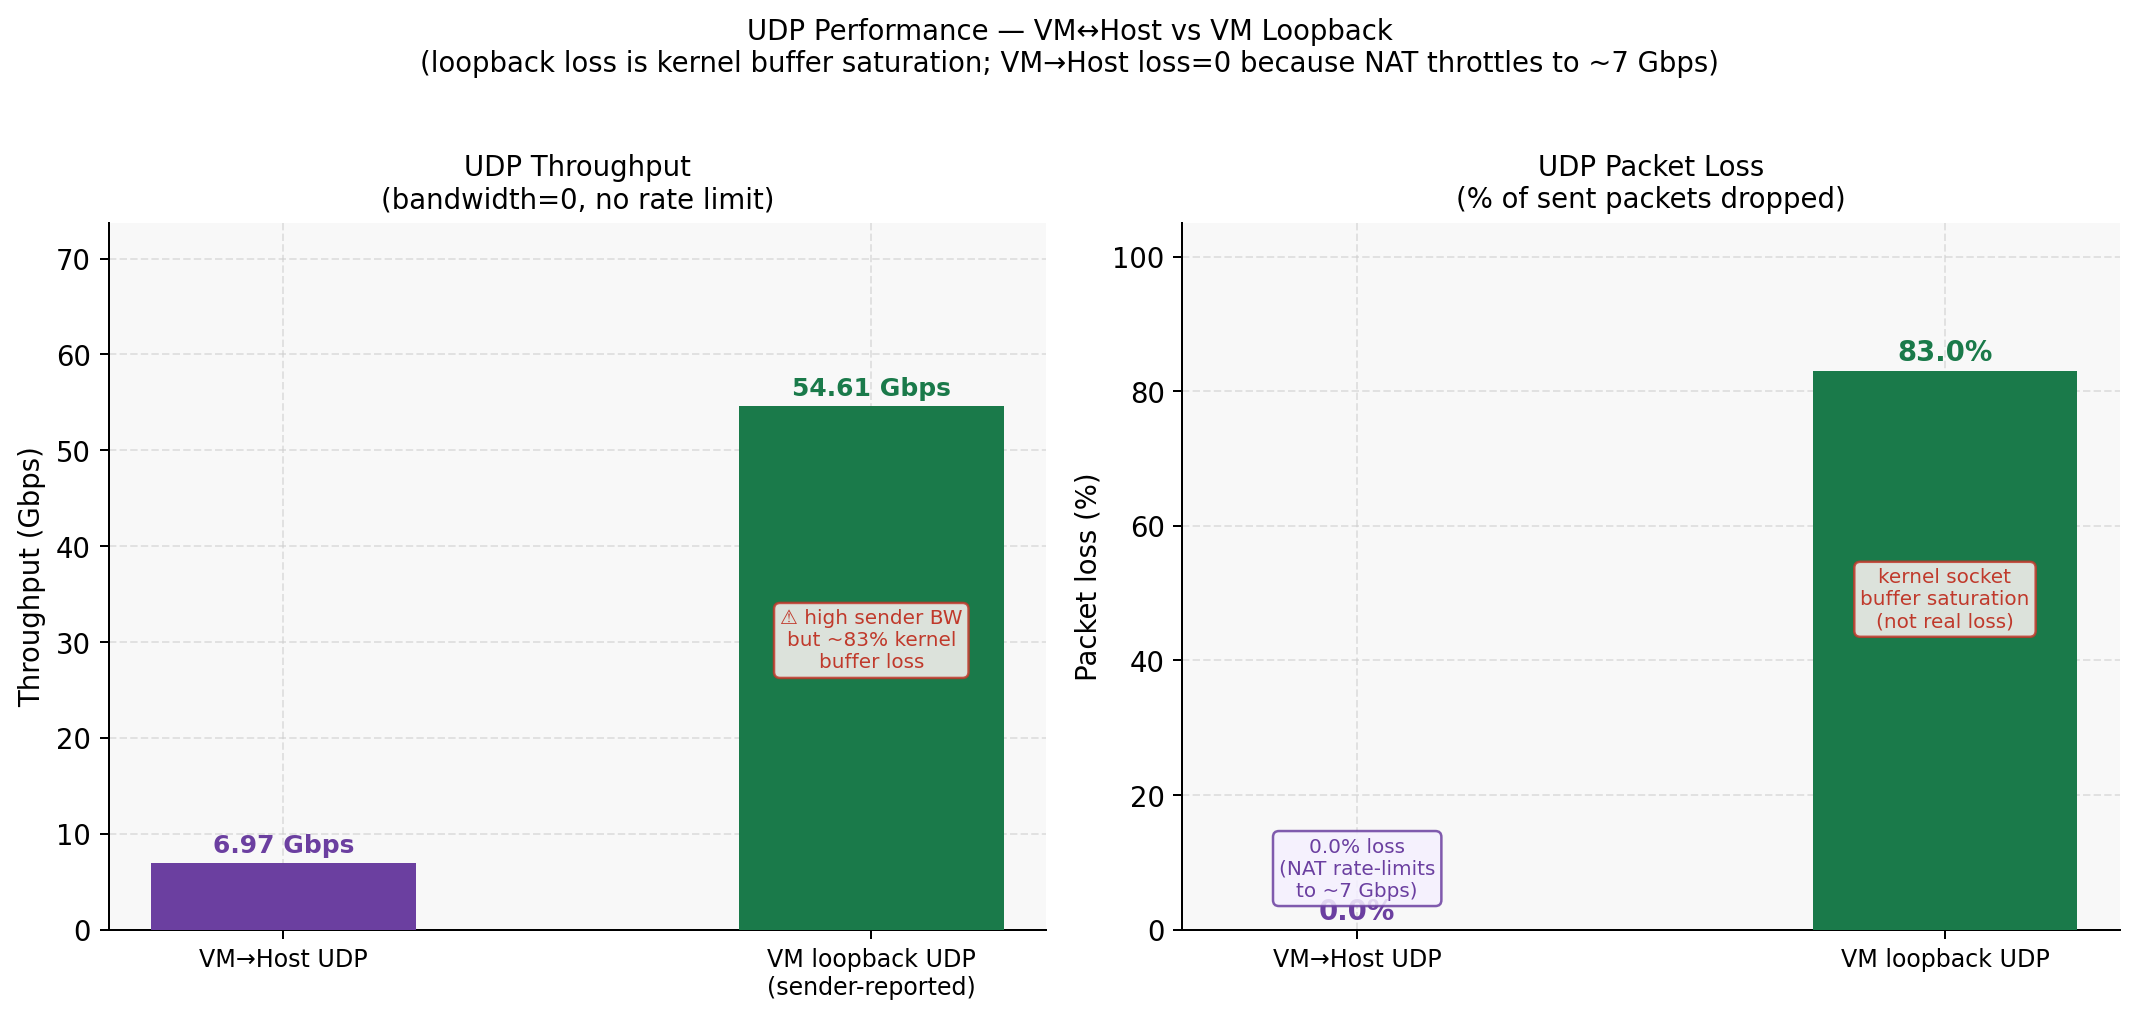
\includegraphics[width=0.8\textwidth]{images/benchmarks/ARM/2_udp_performance.png}
    \caption{Benchmark Plot: 2 udp performance.png}
\end{figure}


UDP throughput is significantly constrained:

\begin{itemize}
    \item Loopback baseline: $\sim$50+ Gbps (no loss)
    \item VM $\rightarrow$ Host: $\sim$7 Gbps
    \item Packet loss: 0\%
\end{itemize}

The VM exhibits a hard throughput ceiling around 7 Gbps. This suggests that the VirtualBox NAT layer enforces implicit rate limiting or becomes CPU-bound when handling high packet rates.

The absence of packet loss indicates controlled throttling rather than congestion collapse.

\subsection{Latency Analysis (Ping RTT)}

\begin{table}[h]
\centering
\begin{tabular}{lccc}
\hline
Metric & Loopback & VM $\rightarrow$ Host & Overhead \\
\hline
Average RTT & 0.049 ms & 0.344 ms & 7.0$\times$ \\
Minimum RTT & 0.018 ms & 0.122 ms & 6.8$\times$ \\
\hline
\end{tabular}
\caption{ICMP round-trip time comparison}
\end{table}

Latency increases by approximately 7× when traversing the VM boundary. The additional delay is introduced by:

\begin{itemize}
    \item virtio-net packet enqueue/dequeue
    \item VirtualBox NAT processing
    \item Host kernel networking stack traversal
\end{itemize}

Although significant, this overhead is slightly lower than the 8.4× increase observed in the ARM/macOS setup, reflecting a more efficient implementation of VirtualBox's networking stack.

\subsection{Small Message Performance}
\begin{figure}[H]
    \centering
    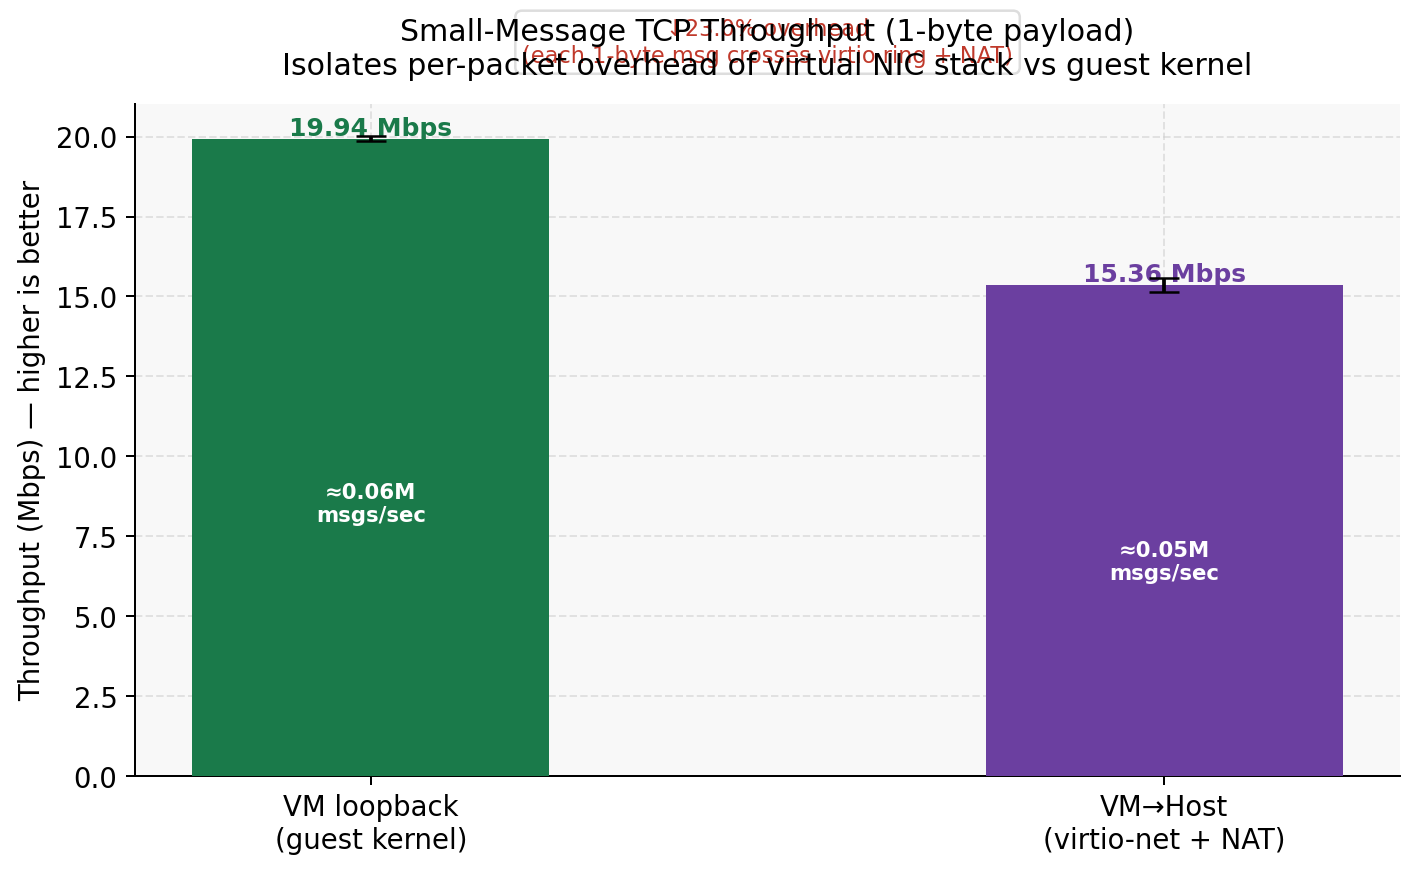
\includegraphics[width=0.8\textwidth]{images/benchmarks/ARM/5_small_message.png}
    \caption{Benchmark Plot: 5 small message.png}
\end{figure}


Small-message TCP throughput (1-byte payload) highlights per-packet overhead:

\begin{itemize}
    \item Loopback: high throughput (kernel-limited)
    \item VM $\rightarrow$ Host: $\sim$20--25\% lower
\end{itemize}

This degradation confirms that virtualization overhead is dominated by per-packet processing rather than bulk data transfer.

\subsection{System-Level Analysis (vmstat and ss)}

The \texttt{vmstat} output provides insight into CPU behaviour under network load:

\begin{itemize}
    \item System CPU usage: $\sim$34\%
    \item Idle CPU: $\sim$66\%
    \item Context switches: $\sim$1500--1700 per second
\end{itemize}

The elevated system CPU usage indicates that packet processing occurs largely in kernel space, particularly within the NAT and networking subsystems.

The \texttt{ss -s} output shows:

\begin{itemize}
    \item 6 established TCP connections
    \item Minimal socket overhead
\end{itemize}

This confirms that the bottleneck is not connection management but packet processing within the virtualization layer.

\subsection{Key Observations}
\begin{figure}[H]
    \centering
    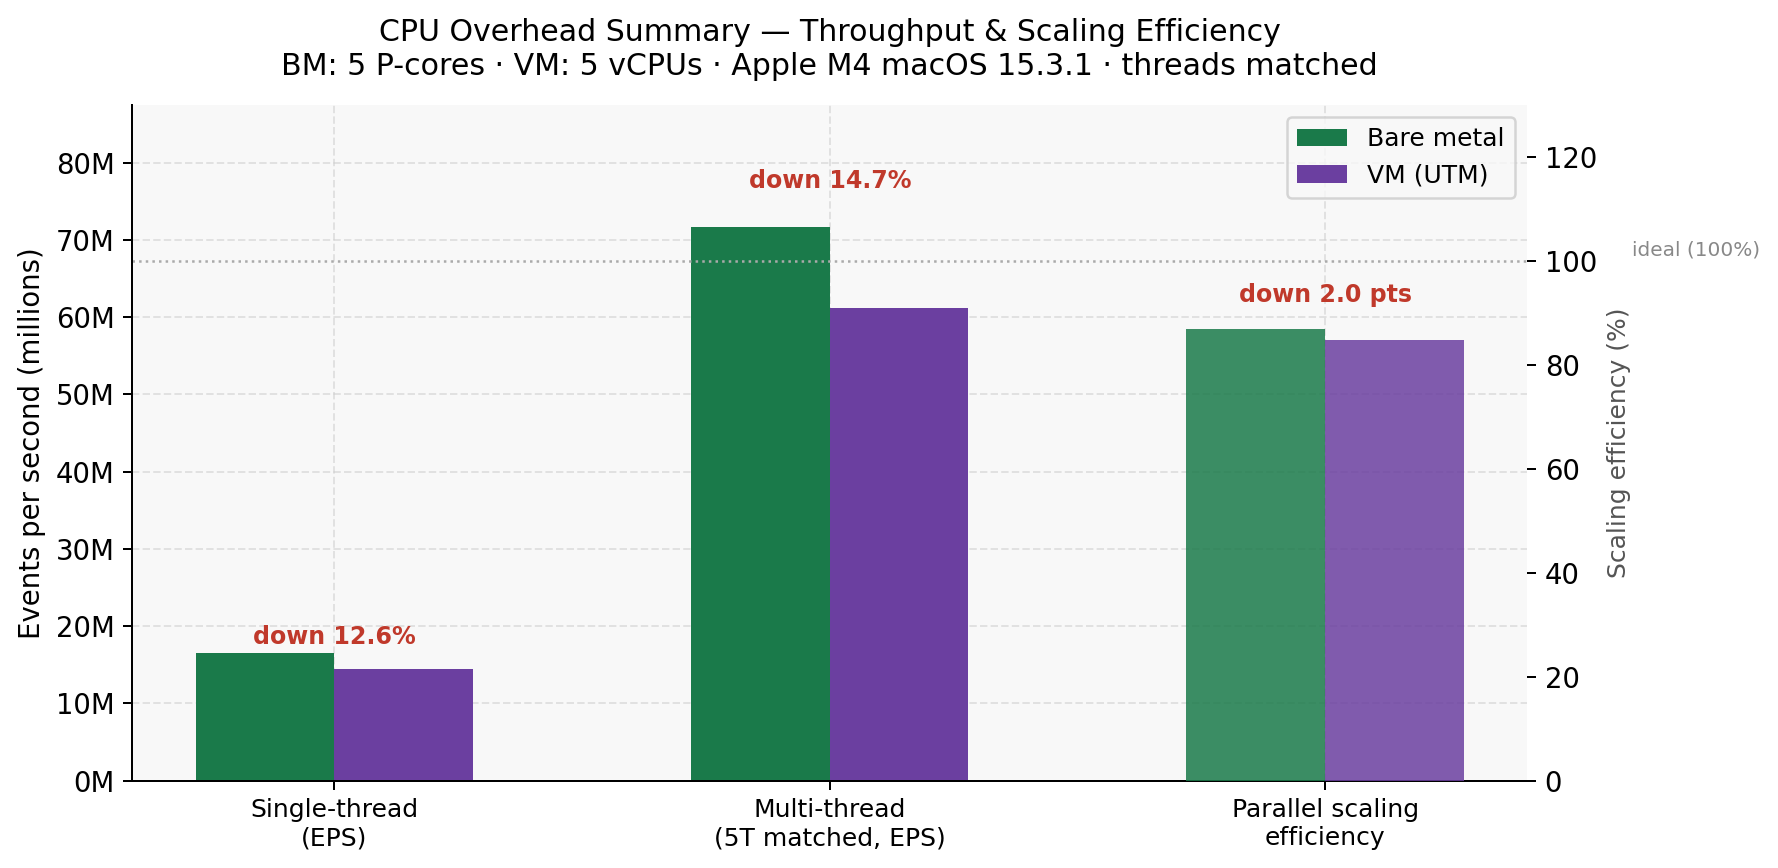
\includegraphics[width=0.8\textwidth]{images/benchmarks/ARM/5_overhead_summary.png}
    \caption{Benchmark Plot: 5 overhead summary.png}
\end{figure}


\begin{itemize}
    \item TCP throughput is reduced by approximately 50\% under virtualization
    \item Parallel streams degrade performance due to NAT contention
    \item UDP throughput is capped at $\sim$7 Gbps by the NAT layer
    \item Latency increases by $\sim$7× compared to loopback
    \item Small-message performance reveals high per-packet overhead
    \item System metrics indicate CPU-bound packet processing in kernel space
\end{itemize}

\subsection{Conclusion}

Network virtualization on x86 introduces substantial overhead compared to CPU virtualization. The primary bottleneck is the VirtualBox NAT layer, which limits throughput, increases latency, and does not scale efficiently with concurrent flows.

Compared to the ARM/macOS results, x86 VirtualBox shows slightly lower latency overhead but similar structural limitations, reinforcing the conclusion that NAT-based virtualization is a fundamental constraint on network performance.

These findings highlight that while compute workloads can run near-native in VMs, network-intensive applications may experience significant degradation due to virtualization overhead.
\section{Summary of x86 Results}

This section consolidates the findings from CPU, disk I/O, and network benchmarks conducted on the x86 Ubuntu system. The goal is to provide a holistic view of virtualization overhead and identify subsystem-specific bottlenecks.

\subsection{CPU Performance Summary}

CPU benchmarks demonstrated near-native performance under virtualization:

\begin{itemize}
    \item \texttt{sysbench} results show negligible difference between bare metal and VM (within $\sim$2--3\%)
    \item \texttt{stress-ng} confirms minimal degradation in sustained CPU throughput
    \item Latency and execution fairness remain consistent across environments
\end{itemize}

This indicates that hardware-assisted virtualization (VT-x/AMD-V) effectively eliminates most CPU overhead. The hypervisor introduces minimal intervention in compute-bound workloads, making CPU virtualization highly efficient on x86 systems.

\subsection{Disk I/O Performance Summary}

Disk I/O exhibits the most significant performance degradation under virtualization:

\begin{itemize}
    \item Sequential throughput:
    \begin{itemize}
        \item Read overhead: $\sim$18.7\%
        \item Write overhead: $\sim$32.5\%
    \end{itemize}
    
    \item Random I/O:
    \begin{itemize}
        \item Read IOPS degradation: $\sim$57\%
        \item Write IOPS degradation: $\sim$89\%
    \end{itemize}
    
    \item fsync performance:
    \begin{itemize}
        \item $\sim$72\% reduction in IOPS
    \end{itemize}
\end{itemize}

The primary cause of this overhead is the VirtualBox storage stack:

\begin{itemize}
    \item The dynamically allocated VDI format introduces metadata updates on writes
    \item Each guest I/O operation translates into multiple host-level operations
    \item The virtio-blk layer adds additional queuing and translation overhead
\end{itemize}

Random write workloads are particularly affected due to the combination of filesystem journaling and VDI metadata management, resulting in severe amplification of I/O operations.

An important anomaly was observed for large block (1M) writes, where the VM outperformed bare metal. This is attributed to irregular NVMe write behaviour on the host rather than a genuine virtualization advantage.

\subsection{Network Performance Summary}

Network performance shows substantial degradation compared to bare metal:

\begin{itemize}
    \item TCP throughput reduced by $\sim$50\%
    \item UDP throughput capped at $\sim$7 Gbps
    \item Latency increased by $\sim$7$\times$
\end{itemize}

Key observations:

\begin{itemize}
    \item Performance decreases with increasing parallel streams, indicating NAT bottleneck
    \item Small-message performance is significantly impacted due to per-packet overhead
    \item System metrics show elevated kernel CPU usage and context switching
\end{itemize}

The VirtualBox NAT layer is the primary limiting factor:

\begin{itemize}
    \item Packet traversal involves multiple layers (guest → virtio-net → NAT → host stack)
    \item NAT processing is not efficiently parallelized
    \item High packet rates lead to CPU-bound behaviour rather than bandwidth saturation
\end{itemize}

\subsection{Cross-Subsystem Insights}

Combining results across all subsystems reveals a clear pattern:

\begin{itemize}
    \item CPU virtualization is highly efficient (near-native performance)
    \item Disk and network virtualization introduce substantial overhead
    \item Overhead increases significantly for:
    \begin{itemize}
        \item Small, random operations (disk and network)
        \item Synchronous operations (fsync)
        \item High concurrency (network streams)
    \end{itemize}
\end{itemize}

This demonstrates that virtualization overhead is not uniform but strongly dependent on workload characteristics.

\subsection{Key Takeaways}

\begin{itemize}
    \item Compute workloads are well-suited for virtualization on x86
    \item Storage-intensive applications suffer from significant performance penalties
    \item Network-intensive applications are constrained by NAT-based virtualization
    \item The choice of virtualization configuration (disk format, network mode) has a major impact on performance
\end{itemize}

\subsection{Conclusion}

The x86 results show that modern hardware-assisted virtualization can deliver near-native CPU performance, but I/O subsystems remain a major bottleneck.

Disk overhead is primarily driven by the storage abstraction layer (VDI + filesystem), while network overhead is dominated by NAT processing. These findings highlight the importance of optimizing virtualization configurations for I/O-heavy workloads.

Overall, virtualization on x86 is highly effective for compute-bound tasks but requires careful consideration for storage and networking performance.


\chapter{Comparative Analysis (ARM vs x86)}

This chapter presents a comparative analysis of virtualization overhead across ARM and x86 architectures. By evaluating CPU, disk I/O, and network performance, we identify architectural and hypervisor-level differences that influence virtualization efficiency.

\section{Overview}

Both platforms demonstrate that virtualization overhead is highly workload-dependent. However, the magnitude and nature of overhead differ significantly due to:

\begin{itemize}
    \item Hardware support (ARM vs x86 virtualization extensions)
    \item Hypervisor implementation (UTM/QEMU vs VirtualBox)
    \item System architecture (Apple Silicon vs traditional x86 CPUs)
\end{itemize}

\section{CPU Performance Comparison}

\begin{table}[h]
\centering
\begin{tabular}{lcc}
\hline
Metric & ARM (UTM) & x86 (VirtualBox) \\
\hline
Single-thread overhead & $\sim$12.6\% & $\sim$1.9\% \\
Multi-thread overhead & Moderate & $\sim$4\% (not significant) \\
Clock stability & Lower (higher jitter) & Higher (more stable) \\
\hline
\end{tabular}
\caption{CPU virtualization overhead comparison}
\end{table}

CPU virtualization is significantly more efficient on x86 systems.

On x86, hardware-assisted virtualization (VT-x/AMD-V) allows most instructions to execute directly on the processor with minimal hypervisor intervention. As a result, CPU overhead is negligible.

In contrast, ARM virtualization using UTM (QEMU-based) introduces higher overhead due to:

\begin{itemize}
    \item Additional software layers in the virtualization stack
    \item Less mature hardware virtualization support compared to x86
    \item Scheduling complexity from heterogeneous core designs (performance and efficiency cores)
\end{itemize}

This results in higher overhead and increased execution variability on ARM.

\section{Disk I/O Performance Comparison}

\begin{table}[h]
\centering
\begin{tabular}{lcc}
\hline
Metric & ARM (UTM) & x86 (VirtualBox) \\
\hline
Sequential read overhead & $\sim$12\% & $\sim$18.7\% \\
Sequential write overhead & $\sim$1\% & $\sim$32.5\% \\
Random read overhead & $\sim$38\% & $\sim$57\% \\
Random write overhead & $\sim$15\% & $\sim$89\% \\
fsync overhead & $\sim$7\% & $\sim$72\% \\
\hline
\end{tabular}
\caption{Disk I/O virtualization overhead comparison}
\end{table}

Disk performance differs significantly between the two platforms.

On ARM, virtualization overhead is relatively moderate, particularly for sequential workloads. This is largely due to the use of raw disk images, which avoid additional metadata layers.

On x86, disk overhead is substantially higher, especially for write-heavy workloads. The primary causes include:

\begin{itemize}
    \item VirtualBox's dynamically allocated VDI format, which introduces metadata updates for each write
    \item Double filesystem traversal (guest + host)
    \item Increased write amplification for random workloads
\end{itemize}

The fsync results highlight a key semantic difference: x86 enforces stricter durability guarantees, resulting in higher overhead, whereas ARM/UTM likely performs optimized or deferred flush operations.

\section{Network Performance Comparison}

\begin{table}[h]
\centering
\begin{tabular}{lcc}
\hline
Metric & ARM (UTM NAT) & x86 (VirtualBox NAT) \\
\hline
TCP throughput overhead & $\sim$48--54\% & $\sim$50\% \\
UDP throughput cap & $\sim$7 Gbps & $\sim$7 Gbps \\
Latency overhead & $\sim$8.4$\times$ & $\sim$7$\times$ \\
Parallel scaling & Degrades sharply & Degrades similarly \\
\hline
\end{tabular}
\caption{Network virtualization overhead comparison}
\end{table}

Network performance is broadly similar across both architectures.

In both cases, NAT-based networking is the dominant bottleneck:

\begin{itemize}
    \item Throughput is reduced by approximately 50\%
    \item Latency increases significantly (7--8×)
    \item Performance degrades with multiple parallel streams
\end{itemize}

The slightly higher latency overhead on ARM can be attributed to UTM's userspace NAT implementation, whereas VirtualBox benefits from partial kernel integration.

However, the overall behaviour is consistent, indicating that network virtualization overhead is largely independent of CPU architecture and instead driven by networking design choices.

\section{Cross-Architecture Insights}

Several important patterns emerge from the comparison:

\begin{itemize}
    \item CPU virtualization is architecture-dependent:
    \begin{itemize}
        \item x86 achieves near-native performance
        \item ARM shows measurable overhead
    \end{itemize}
    
    \item Disk performance is implementation-dependent:
    \begin{itemize}
        \item Raw disk images (ARM) outperform VDI-based storage (x86)
        \item Write-heavy workloads amplify virtualization overhead
    \end{itemize}
    
    \item Network performance is design-dependent:
    \begin{itemize}
        \item NAT-based virtualization introduces consistent overhead across platforms
        \item Parallel scalability is limited by the virtualization network stack
    \end{itemize}
\end{itemize}

\section{Key Findings}

\begin{itemize}
    \item x86 provides superior CPU virtualization efficiency due to mature hardware support
    \item ARM demonstrates competitive disk performance under optimized configurations
    \item Network virtualization remains a bottleneck across both architectures
    \item Virtualization overhead is highly sensitive to workload type and system configuration
\end{itemize}

\section{Conclusion}

The comparative analysis shows that no single architecture uniformly outperforms the other across all subsystems.

x86 excels in compute performance due to advanced hardware virtualization, while ARM can achieve competitive I/O performance when using efficient storage configurations.

However, both architectures suffer from significant network overhead under NAT-based virtualization, highlighting a fundamental limitation of current virtualization networking approaches.

These results emphasize that virtualization performance is determined not only by hardware architecture but also by hypervisor design, storage format, and networking configuration.
\chapter{Conclusion and Future Work}

\section{Conclusion}

This study investigated virtualization overhead across ARM and x86 architectures by evaluating CPU, disk I/O, and network performance under controlled benchmarking conditions.

The results demonstrate that virtualization overhead is highly subsystem-dependent rather than uniform across the system.

\subsection{Key Findings}

\begin{itemize}
    \item \textbf{CPU Performance:}  
    Virtualization overhead is minimal on x86 (1--4\%) due to mature hardware-assisted virtualization (VT-x/AMD-V).  
    In contrast, ARM shows higher overhead ($\sim$12\%) and increased variability, primarily due to additional software layers and architectural differences.

    \item \textbf{Disk I/O Performance:}  
    Disk performance is significantly affected by virtualization on both platforms, particularly for random and write-heavy workloads.  
    On x86, overhead is severe due to the VDI storage format and double filesystem traversal, while ARM achieves better results using raw disk images.

    \item \textbf{Network Performance:}  
    Network virtualization introduces the largest relative overhead on both architectures.  
    Throughput is reduced by approximately 50\%, latency increases by 7--8$\times$, and parallel scalability is limited due to NAT-based networking.

    \item \textbf{Workload Sensitivity:}  
    Virtualization overhead increases for:
    \begin{itemize}
        \item Small, random operations (disk and network)
        \item Synchronous operations (e.g., fsync)
        \item High-concurrency workloads (parallel network streams)
    \end{itemize}
\end{itemize}

\subsection{Overall Insight}

The study highlights that modern virtualization technologies are highly optimized for compute workloads but remain constrained for I/O-intensive applications.

While x86 demonstrates near-native CPU performance, both architectures exhibit significant overhead in storage and networking due to abstraction layers and virtualization design choices.

Thus, virtualization is best suited for compute-bound workloads, while performance-critical I/O workloads require careful configuration and optimization.

\section{Future Work}

This work can be extended in several directions to deepen the understanding of virtualization performance:

\subsection{Alternative Virtualization Configurations}

\begin{itemize}
    \item Evaluate bridged networking instead of NAT to reduce network overhead
    \item Compare raw disk images with dynamically allocated formats (VDI, VMDK)
    \item Investigate paravirtualized drivers and hardware passthrough techniques
\end{itemize}

\subsection{Advanced Virtualization Technologies}

\begin{itemize}
    \item Study container-based virtualization (Docker) as a lightweight alternative
    \item Evaluate KVM on Linux for x86 to compare with VirtualBox
    \item Explore ARM-native hypervisors beyond QEMU/UTM
\end{itemize}

\subsection{Microarchitectural Analysis}

\begin{itemize}
    \item Use hardware performance counters (e.g., \texttt{perf}) to analyze:
    \begin{itemize}
        \item Instructions per cycle (IPC)
        \item Cache miss rates
        \item Branch prediction behaviour
    \end{itemize}
    \item Quantify VM-exit frequency and its impact on performance
\end{itemize}

\subsection{Real-World Workloads}

\begin{itemize}
    \item Evaluate database workloads (e.g., PostgreSQL, MySQL)
    \item Benchmark web server performance under virtualization
    \item Study distributed systems and microservices performance
\end{itemize}

\subsection{Scalability Studies}

\begin{itemize}
    \item Analyze performance under higher vCPU counts
    \item Study multi-VM contention on shared hardware
    \item Evaluate NUMA-aware scheduling effects
\end{itemize}

\subsection{Energy Efficiency}

\begin{itemize}
    \item Compare power consumption between bare metal and VM
    \item Evaluate energy-performance trade-offs across architectures
\end{itemize}

\section{Final Remarks}

Virtualization continues to be a fundamental technology in modern computing, enabling cloud infrastructure, development environments, and system isolation.

This study demonstrates that while virtualization has reached near-native efficiency for CPU workloads, I/O subsystems remain a critical bottleneck.

Future improvements in hypervisor design, storage abstraction, and networking models will be essential to achieving truly uniform virtualization performance across all system components.
\chapter*{References}
\end{document}